%% LyX 2.2.3 created this file.  For more info, see http://www.lyx.org/.
%% Do not edit unless you really know what you are doing.
\documentclass[english]{article}
\usepackage[T1]{fontenc}
\usepackage[latin9]{inputenc}
\usepackage{array}
\usepackage{graphicx}

\makeatletter

%%%%%%%%%%%%%%%%%%%%%%%%%%%%%% LyX specific LaTeX commands.
%% Because html converters don't know tabularnewline
\providecommand{\tabularnewline}{\\}

\makeatother

\usepackage{babel}
\begin{document}
\noindent \begin{center}
\includegraphics[scale=0.15]{\string"images/GitHub Banner\string".png}
\par\end{center}
\begin{quote}
\begin{center}
{\Huge{}Travlendar+}
\par\end{center}{\Huge \par}
\begin{center}
{\Large{}Requirement Analysis Specification Document}
\par\end{center}{\Large \par}
\begin{center}
Calzavara Filippo, Filaferro Giovanni, Benedetto Maria Nespoli
\par\end{center}

\end{quote}
\begin{center}
Version 1.0.0
\par\end{center}

\bigskip{}
\noindent \begin{center}

\includegraphics[width=3cm]{images/PolimiLogo}
\par\end{center}

\pagebreak{}\tableofcontents{}

\pagebreak{}

\section{Introduction}

\subsection{Purpose}

This document is the Requirements Analysis Specification Document
(RASD) for Travlendar+, the system assigned to be developed for the
mandatory project. The document describes the characteristics of the
system, both functional and non-functional requirements for the software,
design constrains and system interfaces. It is addressed to be read
by the developers that will implement the final system.

\subsection{Scope}

The aim of this project is to create a smart calendar-based application
that people can use to reduce delays at the appointments and supporting
the users by identifying the best mobility option. People create appointments
and they get notified in case they will not be on time for it. Moreover,
the system needs to take into account weather forecast as well as
strike days. Furthermore, the users should be able to adapt settings
based on their preferences, such as walking-time constrains or a more
eco-friendly way of transportation, and the possibility to define
flexible appointments that given a window of time and a duration an
arrangement of the schedule is proposed. Finally, the system should
provide the user of a ticket or locate the closest car/bike sharing
vehicle if it is the mean of transportation chosen.

\subsubsection{Goals}
\begin{itemize}
\item {[}G0{]} Allow people to use the app without a login function
\item {[}G1{]} Allow people to view the daily schedule with coming up events
at the top
\item {[}G2{]} Allow people to view previous events
\item {[}G3{]} Allow people to view the details of each event
\begin{itemize}
\item {[}G3.1{]} Allow people to get travel information for a particular
event
\begin{itemize}
\item {[}G3.1.1{]} Allow people to get the ETA to the appointment
\end{itemize}
\item {[}G3.2{]} Allow people to explore a specific route
\begin{itemize}
\item {[}G3.2.1{]} Allow people to purchase the transit ticket
\item {[}G3.2.2{]} Allow people to open the sharing services/ride provider's
app and call the vehicle
\end{itemize}
\item {[}G3.3{]} Allow people to eventually view the purchased transit ticket
\end{itemize}
\item {[}G4{]} Allow the users to create an event
\begin{itemize}
\item {[}G4.1{]} Allow the user to define a name/description of the appointment
\item {[}G4.2{]} Allow the user to define the location
\item {[}G4.3{]} Allow users to set a flexible timing
\begin{itemize}
\item {[}G4.3.1{]} Allow the user to select a time window in which the event
will occur
\item {[}G4.3.2{]} Allow the user to select how long the event will last
\end{itemize}
\item {[}G4.4{]} Allow the user to set a starting time and ending time on
non-flexible events
\item {[}G4.5{]} Allow the user to repeat the event regularly throughout
the week
\item {[}G4.6{]} Allow the user to assign the event to a specific calendar
\item {[}G4.7{]} Allow the user to define the mean of transportations that
he/she wants to use for the event
\end{itemize}
\item {[}G5{]} Allow people to see daily events on a map
\begin{itemize}
\item {[}G5.1{]} Allow the user to have information about the status of
the journey to make in order to reach the appointment's location 
\item {[}G5.2{]} Allow the user to see previous daily events on a map
\end{itemize}
\item {[}G6{]} Allow the user to set preferences
\begin{itemize}
\item {[}G6.1{]} Allow the user to set the eco-friendly mode
\item {[}G6.2{]} Allow the user to set the walkable distance limit
\item {[}G6.3{]} Allow the user to set the maximum biking range
\item {[}G6.4{]} Allow the users to set the owned bike and/or bike sharing
providers
\item {[}G6.5{]} Allow the users to set a time range in which they can take
public transits
\item {[}G6.6{]} Allow the users to set if they own a car and/or their favorite
car sharing providers
\item {[}G6.7{]} Allow the users to set the preferred ride sharing service
\end{itemize}
\item {[}G7{]} Allow the users to create calendars
\begin{itemize}
\item {[}G7.1{]} Allow the users to color calendar
\item {[}G7.2{]} Allow the users to change calendar's color and name
\end{itemize}
\item {[}G8{]} Notify the user that it's time to leave for the appointment
\end{itemize}

\subsection{Definitions, Acronyms, Abbreviations}

\subsubsection{Definitions}

\begin{tabular}{|c|c|}
\hline 
Definition & Explanation\tabularnewline
\hline 
\hline 
Appointment & A period of time in which something take place at a certain time\tabularnewline
\hline 
Travlendar+ & The name of the platform to develop\tabularnewline
\hline 
Event & A synonym for appointment \tabularnewline
\hline 
System & A synonym of Travlendar+\tabularnewline
\hline 
Up Coming Event & A particular event that is expected to occur soon\tabularnewline
\hline 
Up Next Event & A synonym of Up Coming\tabularnewline
\hline 
User & A potential utilizer of this project\tabularnewline
\hline 
Ride & A service performed by a ride-sharing company and Cabs\tabularnewline
\hline 
\end{tabular}

\subsubsection{Acronyms}

\begin{tabular}{|c|c|}
\hline 
Acronym & Explanation\tabularnewline
\hline 
\hline 
GUI & Graphic User Interface\tabularnewline
\hline 
ETA & Estimated time of arrival\tabularnewline
\hline 
API & Application programming interface\tabularnewline
\hline 
RASD & Requirement Analysis and Specification Document\tabularnewline
\hline 
PNR & Passenger name record\tabularnewline
\hline 
QR & Quick Response Code\tabularnewline
\hline 
OS & Operative Systemk\tabularnewline
\hline 
\end{tabular}

\subsubsection{Abbreviations}

\begin{tabular}{|c|c|}
\hline 
Abbreviation & Explanation\tabularnewline
\hline 
\hline 
App & A synonym of Travlendar+\tabularnewline
\hline 
{[}Gn{]} & N-goal\tabularnewline
\hline 
{[}Dn{]} & N-domain assumption\tabularnewline
\hline 
{[}Rn{]} & N-functional requirement\tabularnewline
\hline 
\end{tabular}

\subsection{Revision history}
\begin{itemize}
\item 1.0.0 - Initial Version (16/10/2017) 
\end{itemize}

\subsection{Reference Documents }
\begin{itemize}
\item Specifications document ``Mandatory Project Assignments.pdf''
\item ISO/IEC/IEEE 29148 - IEEE Standard on Requirements Engineering
\item Software Abstractions, MIT Press
\end{itemize}

\subsection{Document Structure}

The paper includes six areas. The first one, is composed by the introductory
information provided in order to give an orientative view of what
this document is about. The second one, provides an overall description
of the project including the features, the characteristics and the
constraints that its development implies. The main body of this paper
is contained in the third section, which assert the requirements and
the design constraints. The paper is equipped with a fourth section
that contains a formal analysis using Alloy. Finally, a fifth and
a sixth section allows the reader to learn the effort spent on this
project by each team member and the references made in the whole paper.

\pagebreak{}

\section{Overall Description}

\subsection{Product perspective}

Travlendar+ is a standalone system that provides the functionality
described in the Product Function Section 2.2. It would implement
external services in order to offer weather forecast, maps services,
sharing systems information, transits and strike information.

\subsubsection{Class Diagram}
\begin{center}
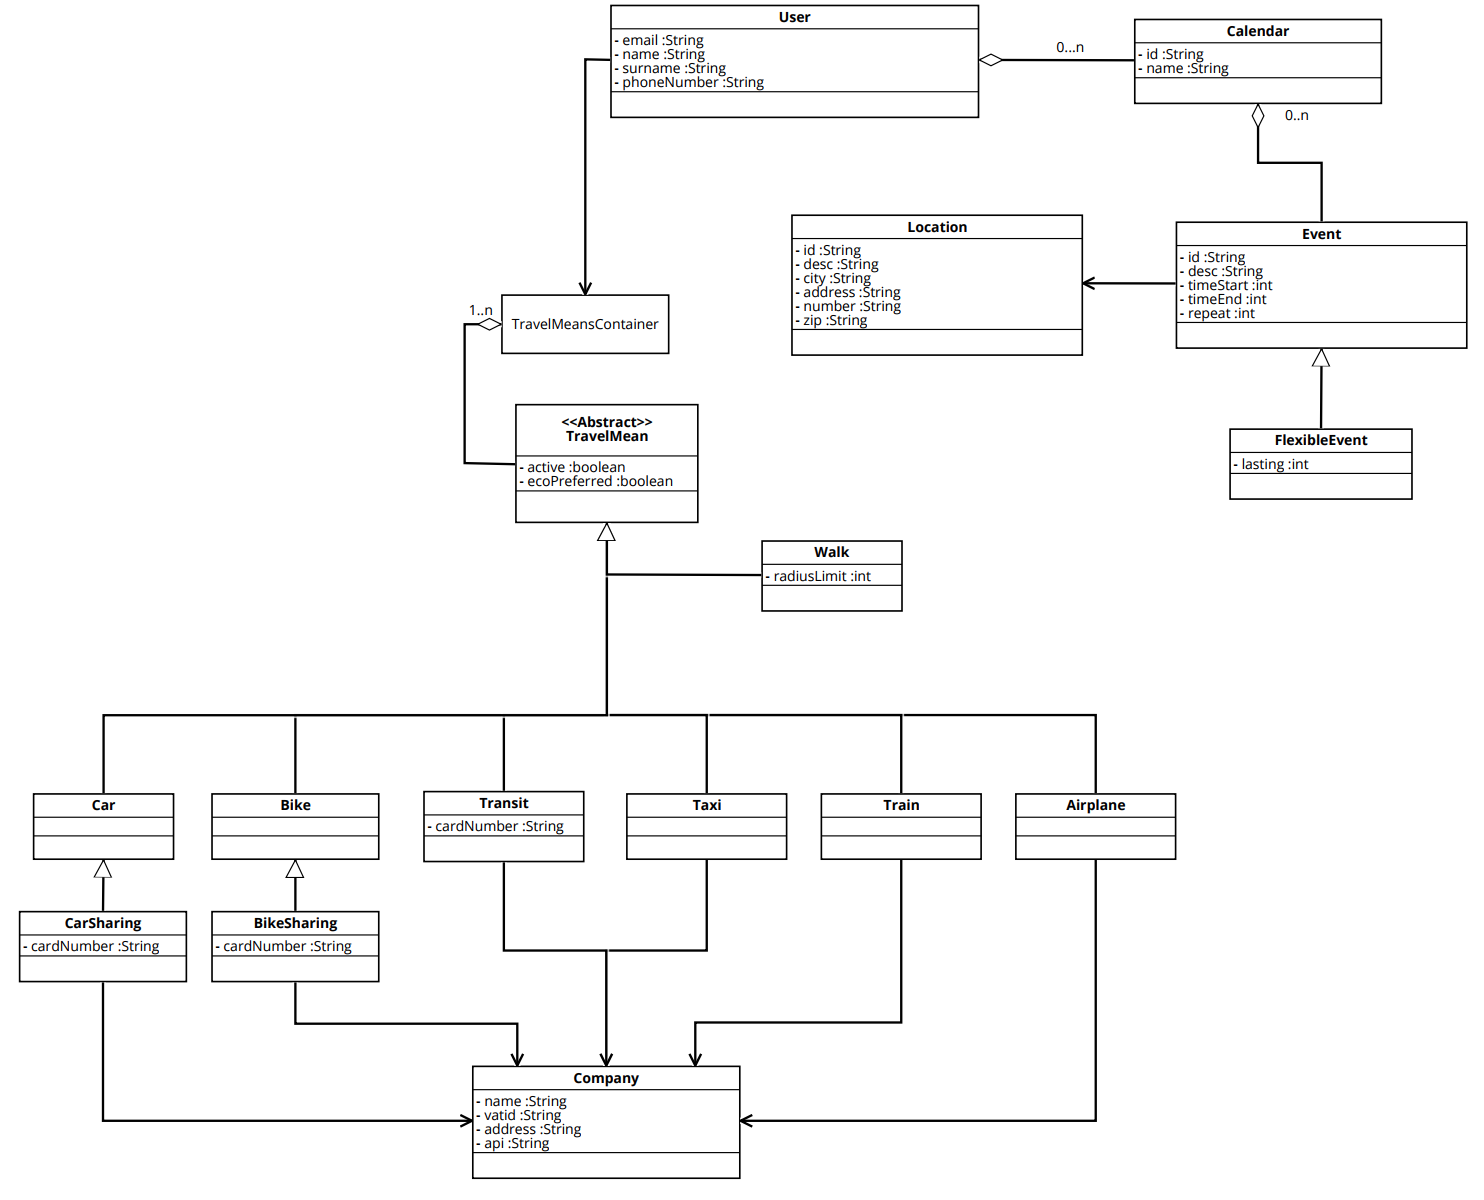
\includegraphics[scale=0.45]{images/CD}
\par\end{center}

\subsubsection{Statechart}

The system is based on two different modes: The active function and
the passive function. The first is in place when the person is actively
using the application and its functionality. The latter is a background
service that runs in order to keep track of the position, other information
and it attract user's attention when a notification is risen.

\textbf{Active mode:}
\begin{center}
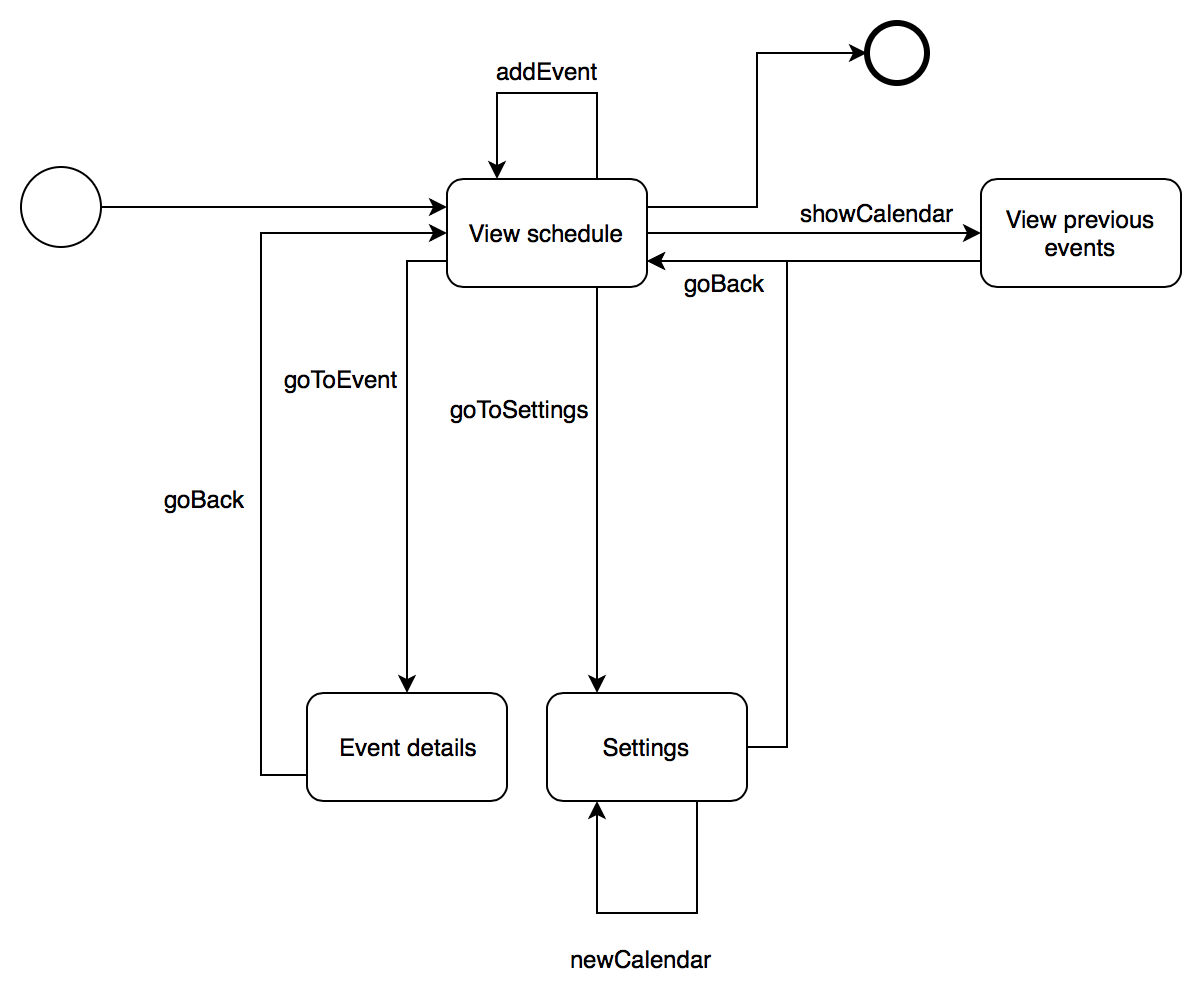
\includegraphics[scale=0.27]{images/SC-active}
\par\end{center}

\textbf{Passive mode:}
\noindent \begin{center}
\hspace*{-2.0cm}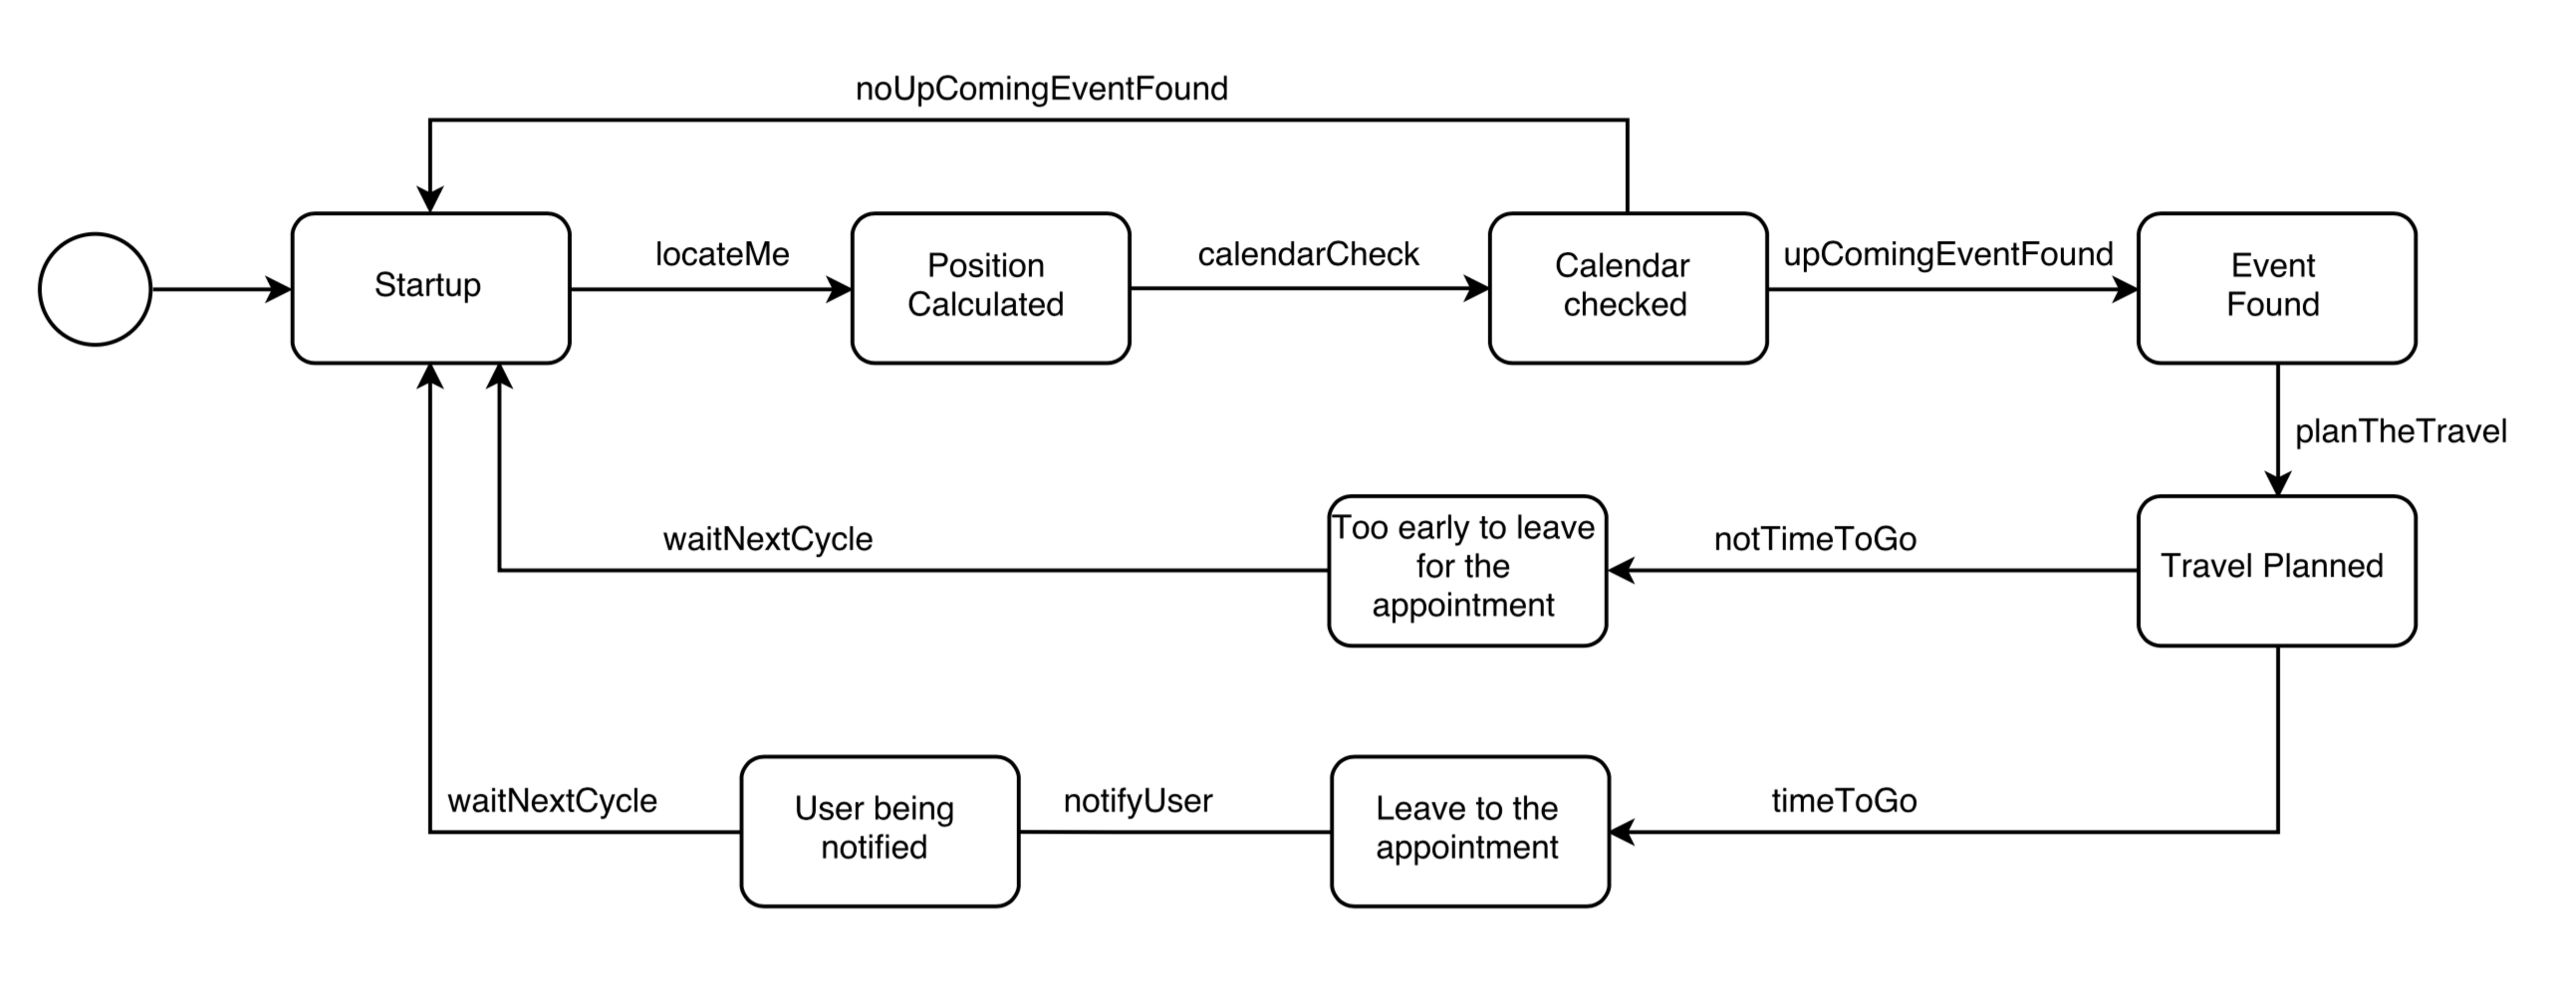
\includegraphics[scale=0.36]{images/SC-passive}
\par\end{center}

\subsection{Product functions}

Each goal described in Section 1.2.1 is function that will be implemented
in the system. We report below the functionalities that require a
further explanation and the boundaries between the system to be developed
and thirty party system.

\subsubsection{Allow people to purchase and view the transit ticket}

The ticket buying system will use regular text messages to send a
purchasing request at the local transit company which reply to our
app with the PNR code of the ticket. This choice of designing was
made to ensure compatibility among every transit provider and to allow
users to pay it by charging the cost of the ticket on their cell phone
credit/bill, letting the carrier provider handling the payment.

When the purchasing is completed, a QR code representing the ticket's
PNR will be displayed on the user's screen.

\subsubsection{Overlapped events}

While creating an event, the system automatically rearrange the schedule
in order to fit all the events in the calendar. In case an event overlaps
another event of the same calendar, an exception is thrown. In case
an event overlaps one event of another calendar nothing happen.

Moreover, an error is shown when the user tries to add an event that
could not be reached in time.

\subsection{User characteristics}

This application is designed to be used by any person that would like
to have a more organized schedule

\subsection{Assumptions, dependencies and constraints}

We assume that: 
\begin{enumerate}
\item The client is using the app through a new generation smartphone
\item The mobile device has a GPS system
\item The mobile device has a regular 3G internet connection available
\item The software is designed to be utilized in Italy, precisely in the
region of Lombardy
\item Public transits companies provide a sms-based purchasing system
\item The user has already logged in to his/her device account (Google or
Apple) so that we can identify him/her by using their unique identifier.
\item Vehicle-sharing/ride-sharing companies' will provide APIs to locate
the nearest vehicle available
\item Weather forecast are provided from an external service through API
\item Calculating the shortest path follows a time-based criteria instead
of a cost-based one
\end{enumerate}

\subsubsection{Interfaces to other applications}

At the first stages of the project, Travlendar+ will not release API
interfaces to the public

\subsubsection{Public transit pass}

The system will not take into consideration whether the person owns
a transit's pass, however it will always allows to buy one or more
transit tickets if asked by the user

\subsubsection{Domain assumption}
\begin{itemize}
\item {[}D1{]} App data are stored remotely and retrieved by multiple devices
\item {[}D2{]} Up coming events' section needs to contain appointments planned
to happen 2h before
\item {[}D3{]} Transportation information are not shown for the past events
\item {[}D4{]} Indications on the ETA, calculated mean of transportation
and time-to-leave are calculated on the current approximative position
\item {[}D5{]} User's position is retrieved using GPS system
\item {[}D6{]} Position is re-calculated every 2 hours, or when a significant
change in GPS position is discovered
\item {[}D7{]} The map can be browsed by the user
\item {[}D8{]} The localization service is available and functionally working
\item {[}D9{]} The map service is reliable
\item {[}D10{]} The button to choose the calendar is, by default, the last
calendar chosen, or the first calendar if the user has never added
an event
\item {[}D11{]} While creating an event, the system must take into account
whether the eco mode has been turned on
\item {[}D12{]} The map can be browsed by the user
\item {[}D13{]} Every preference agrees with the actual record saved in
the database 
\item {[}D14{]} Allowed services have been preinstalled
\item {[}D15{]} The user has always at least one calendar
\item {[}D16{]} Each calendar belongs to only one user
\item {[}D17{]} Each event belongs to only one calendar
\item {[}D18{]} The user won't insert overlapping events
\end{itemize}
\pagebreak{}

\section{Specific Requirements}

\subsection{External Interface Requirements}

\subsubsection{User Interfaces }

\paragraph{Home Screen}

\vspace*{\bigskipamount}
\begin{center}
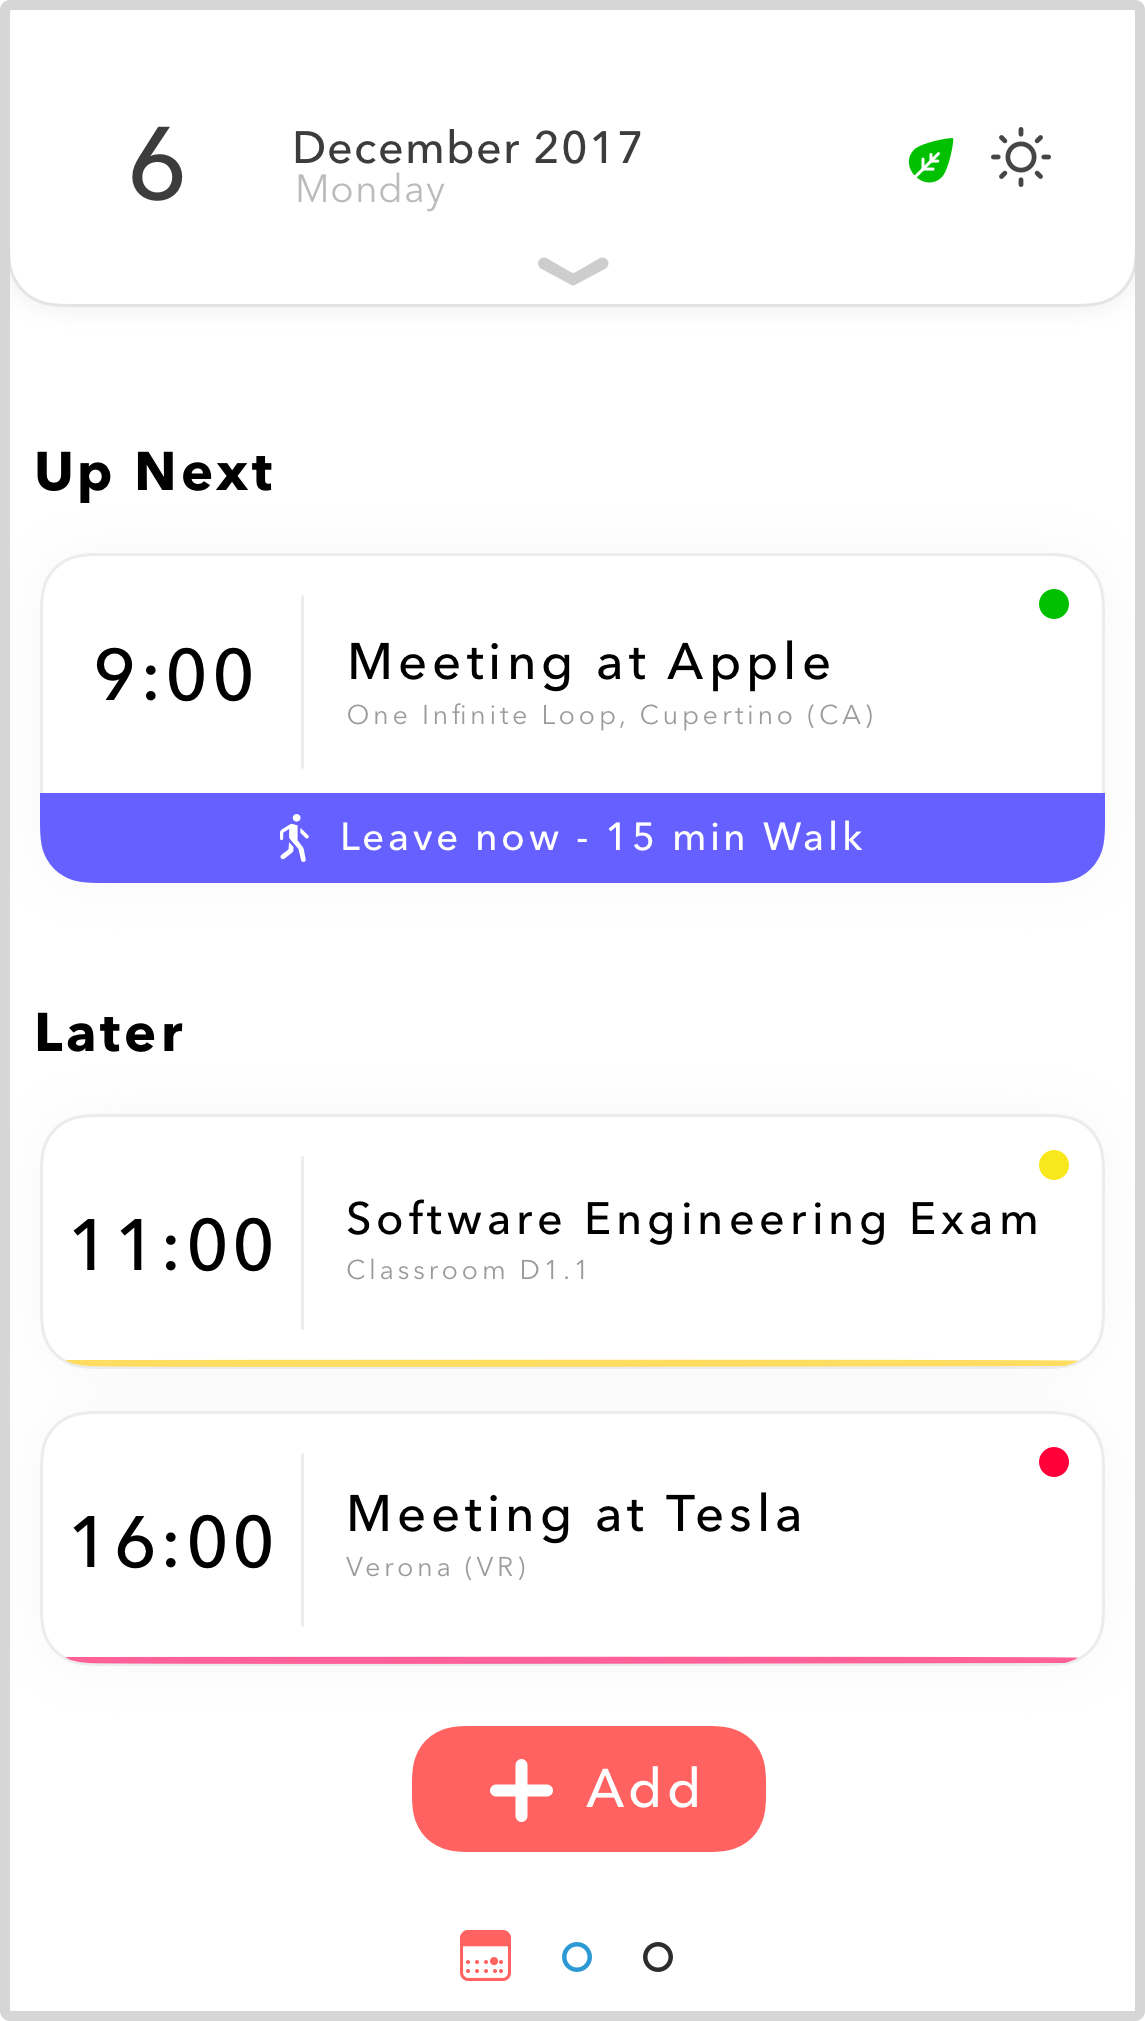
\includegraphics[scale=0.13]{images/Wireframe/2-HomeScr_wired@3x}\enskip{}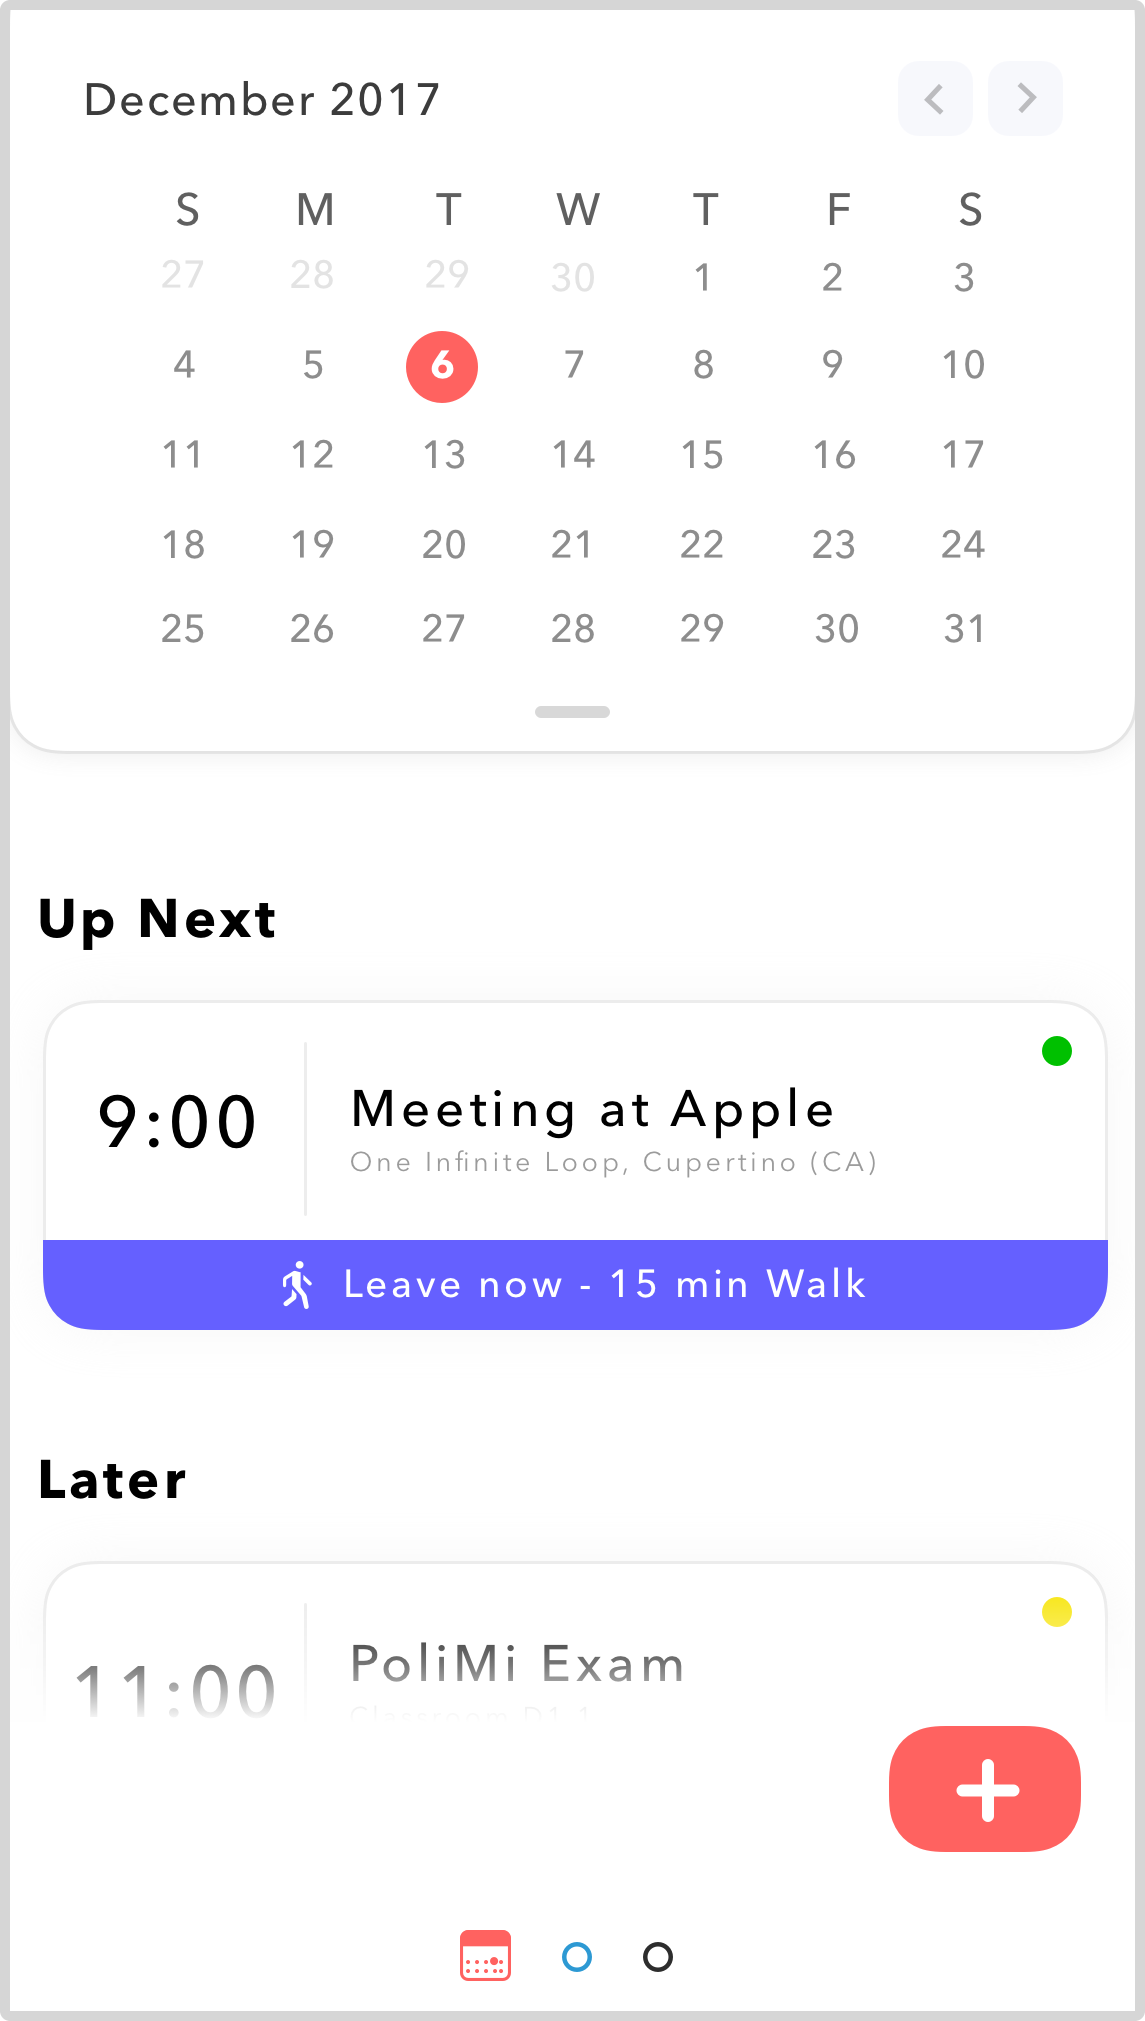
\includegraphics[scale=0.13]{images/Wireframe/3-HomeScreenCalendarExpan_wired@3x}
\par\end{center}

Here is shown the main page that will appear once opened the app.
People can see directly their upcoming events of the day. By pulling
down the top view (where 16 December 2017 is written) they can access
the calendar view (Right Picture) and by tapping on a particular day
the UI re-adapts to that day showing its regarding events. Onto this
page users may see wether the ECO-Friendly mode is enabled (Green
Leaf on top) and the current weather. Furthermore, on the mockup here
proposed the reader may see a suggested route and an ETA for the up
coming event. It is also shown a little dot at the upper right side
of the cell that becomes:
\begin{itemize}
\item \textbf{Green} when the user is on time/early.
\item \textbf{Yellow} when the user will be late if he/she doesn't hurry
up.
\item \textbf{Red} when they will centrally be late or there is a problem
in that route.
\end{itemize}
In each cell there is a small bar on the bottom whom color depends
on calendar's color where the event is saved to.

\paragraph{Event Detail}

\vspace*{\bigskipamount}
\begin{center}
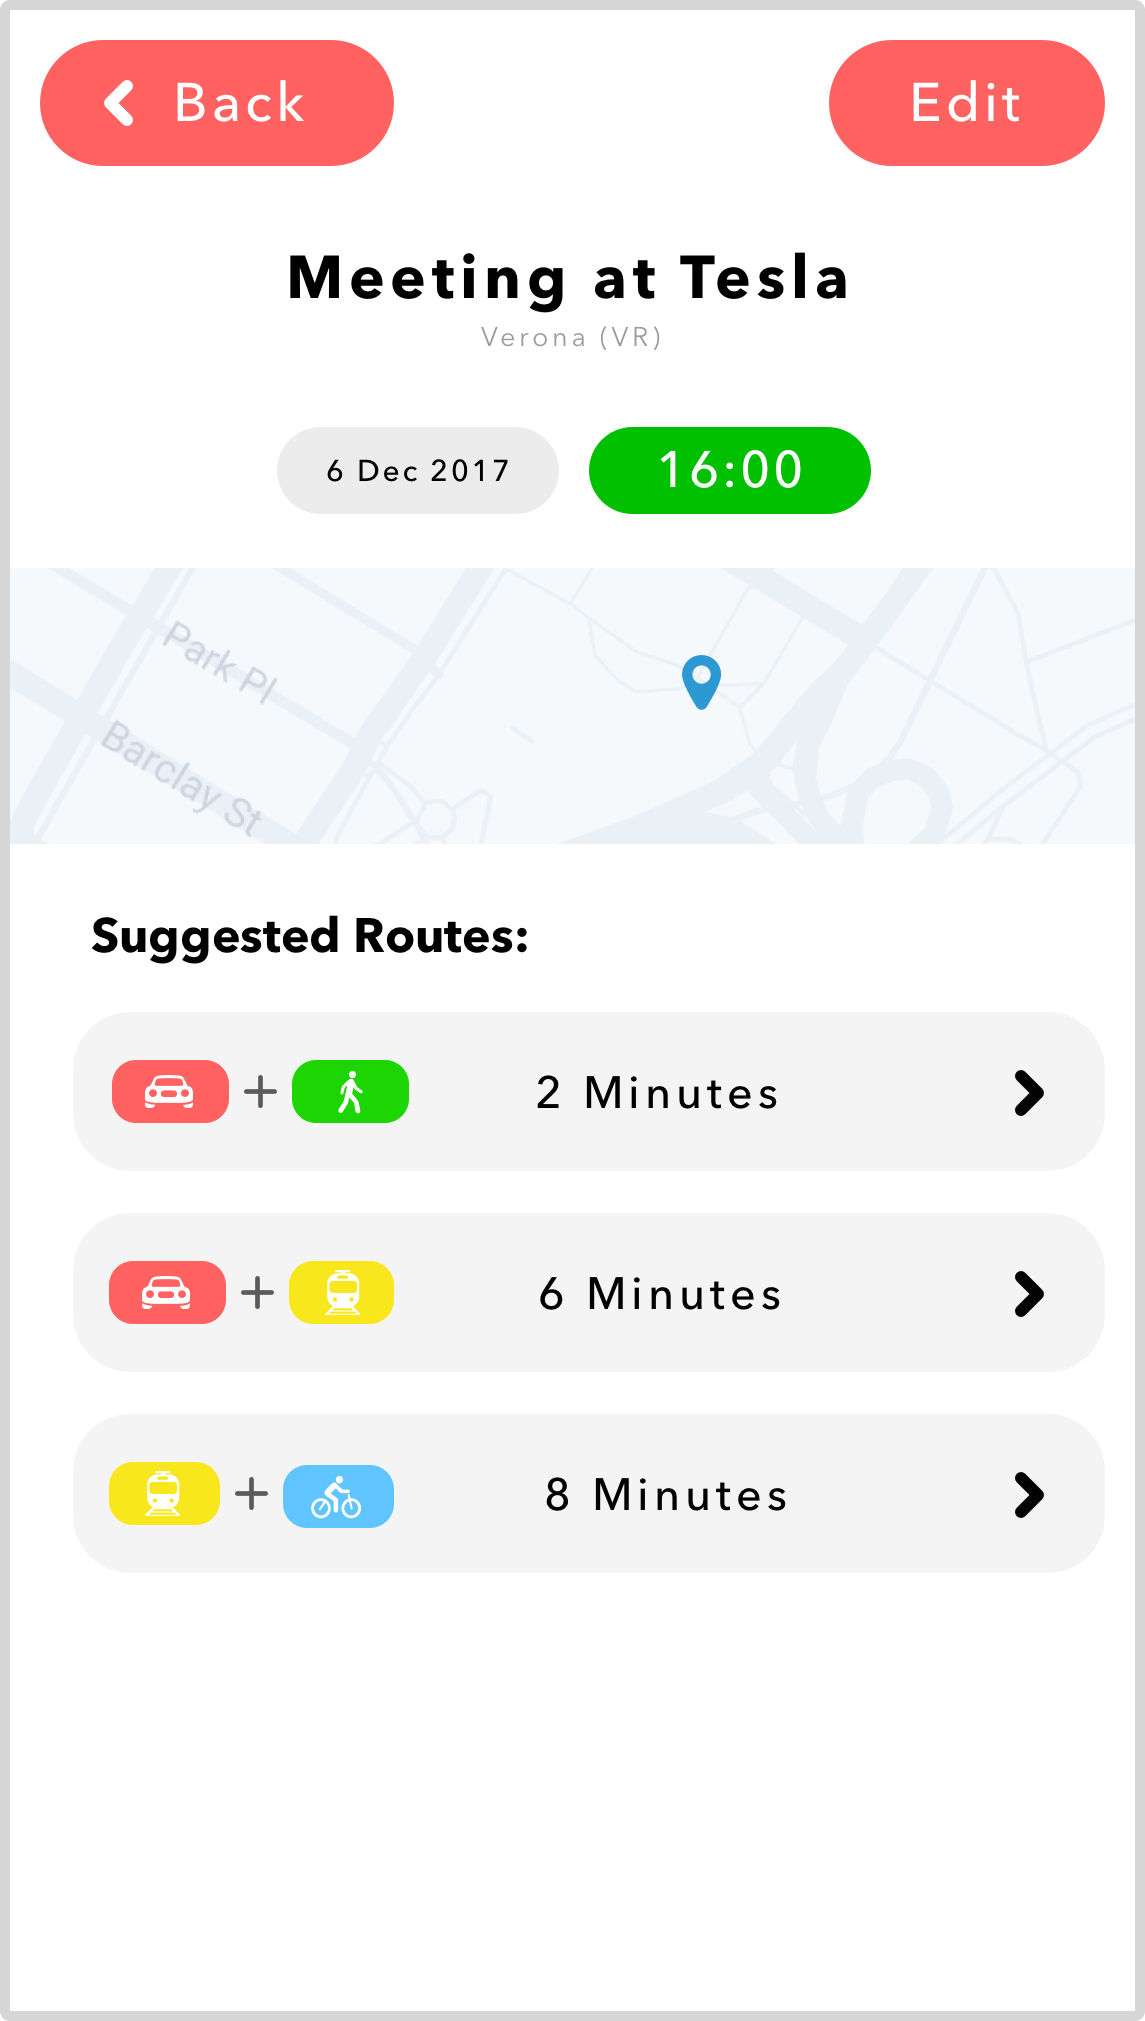
\includegraphics[scale=0.15]{images/Wireframe/4-EventDet_wired@3x}
\par\end{center}

This is the place where, once tapped on an event in the Home Screen,
people can have a fast look at its more interesting details:
\begin{itemize}
\item Basic details of the event such as day, time, position and name.
\item There will be a map view where the location of the event will be shown.
\item Suggested routes (compound ones too) to take based on the user preferences
\end{itemize}
From this view the user is allowed also to edit the event by tapping
the ``Edit'' button.

\pagebreak{}

\paragraph{Event Detail / Route Detail}

\vspace*{\bigskipamount}
\begin{center}
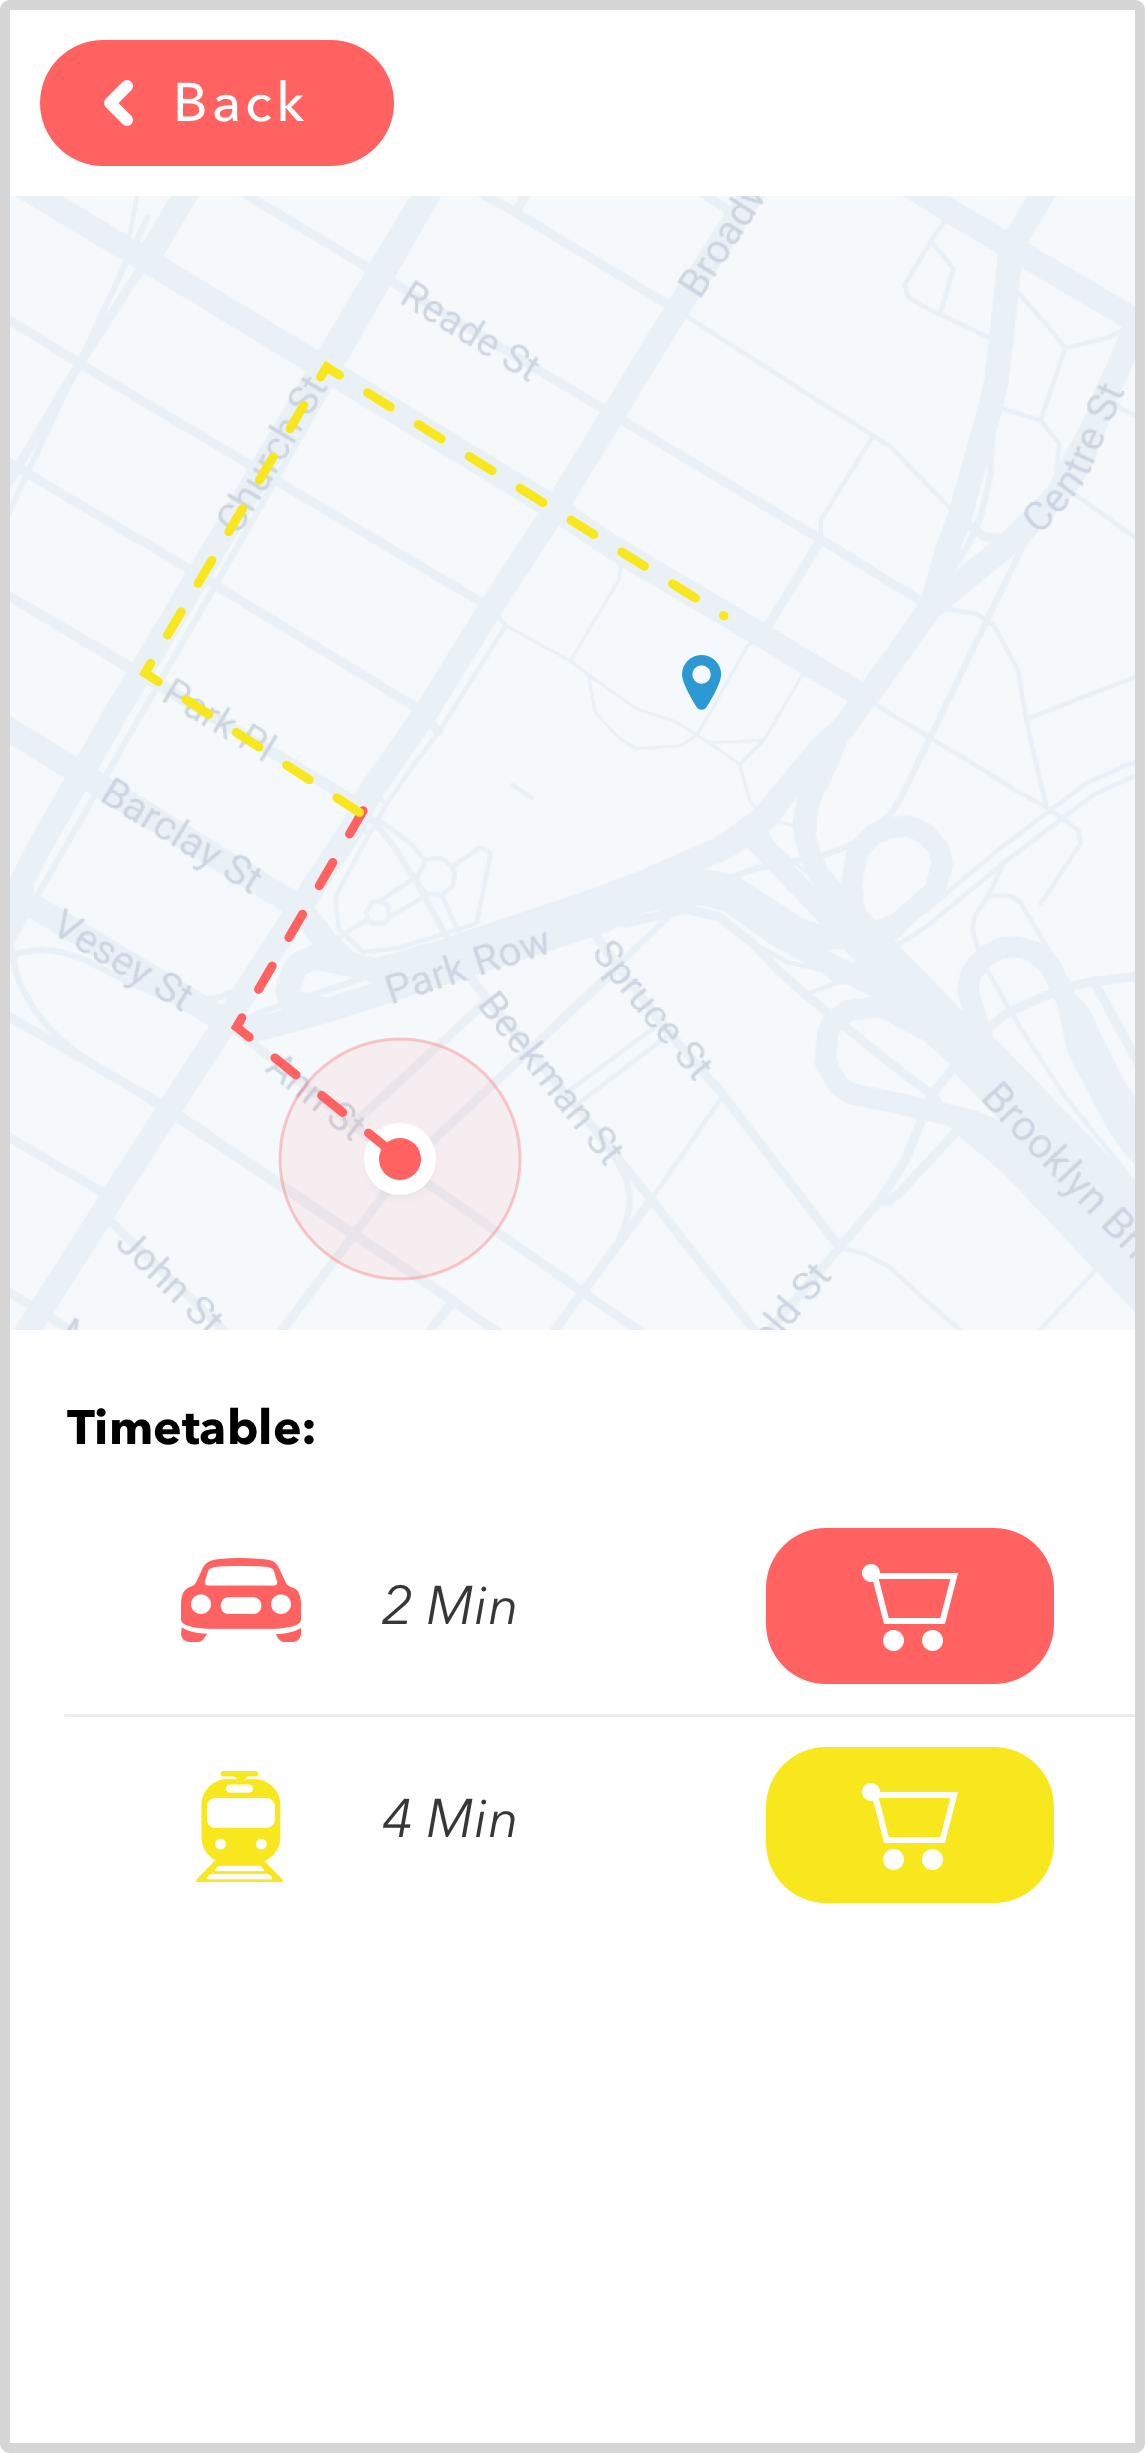
\includegraphics[scale=0.15]{images/Wireframe/6-EventDetail-RouteDet_wired@3x}
\par\end{center}

Just by tapping to one suggested route from ``Event Detail'' view,
the app will present to the user this view in which they can look
at the routes to reach the event.

In particular all the parts composing the route are shown on map and
just by tapping the button on the right of each cell the app will
prompt the user to buy a ticket.

\pagebreak{}

\paragraph{Event Detail / Ticket Bought}

\vspace*{\bigskipamount}
\begin{center}
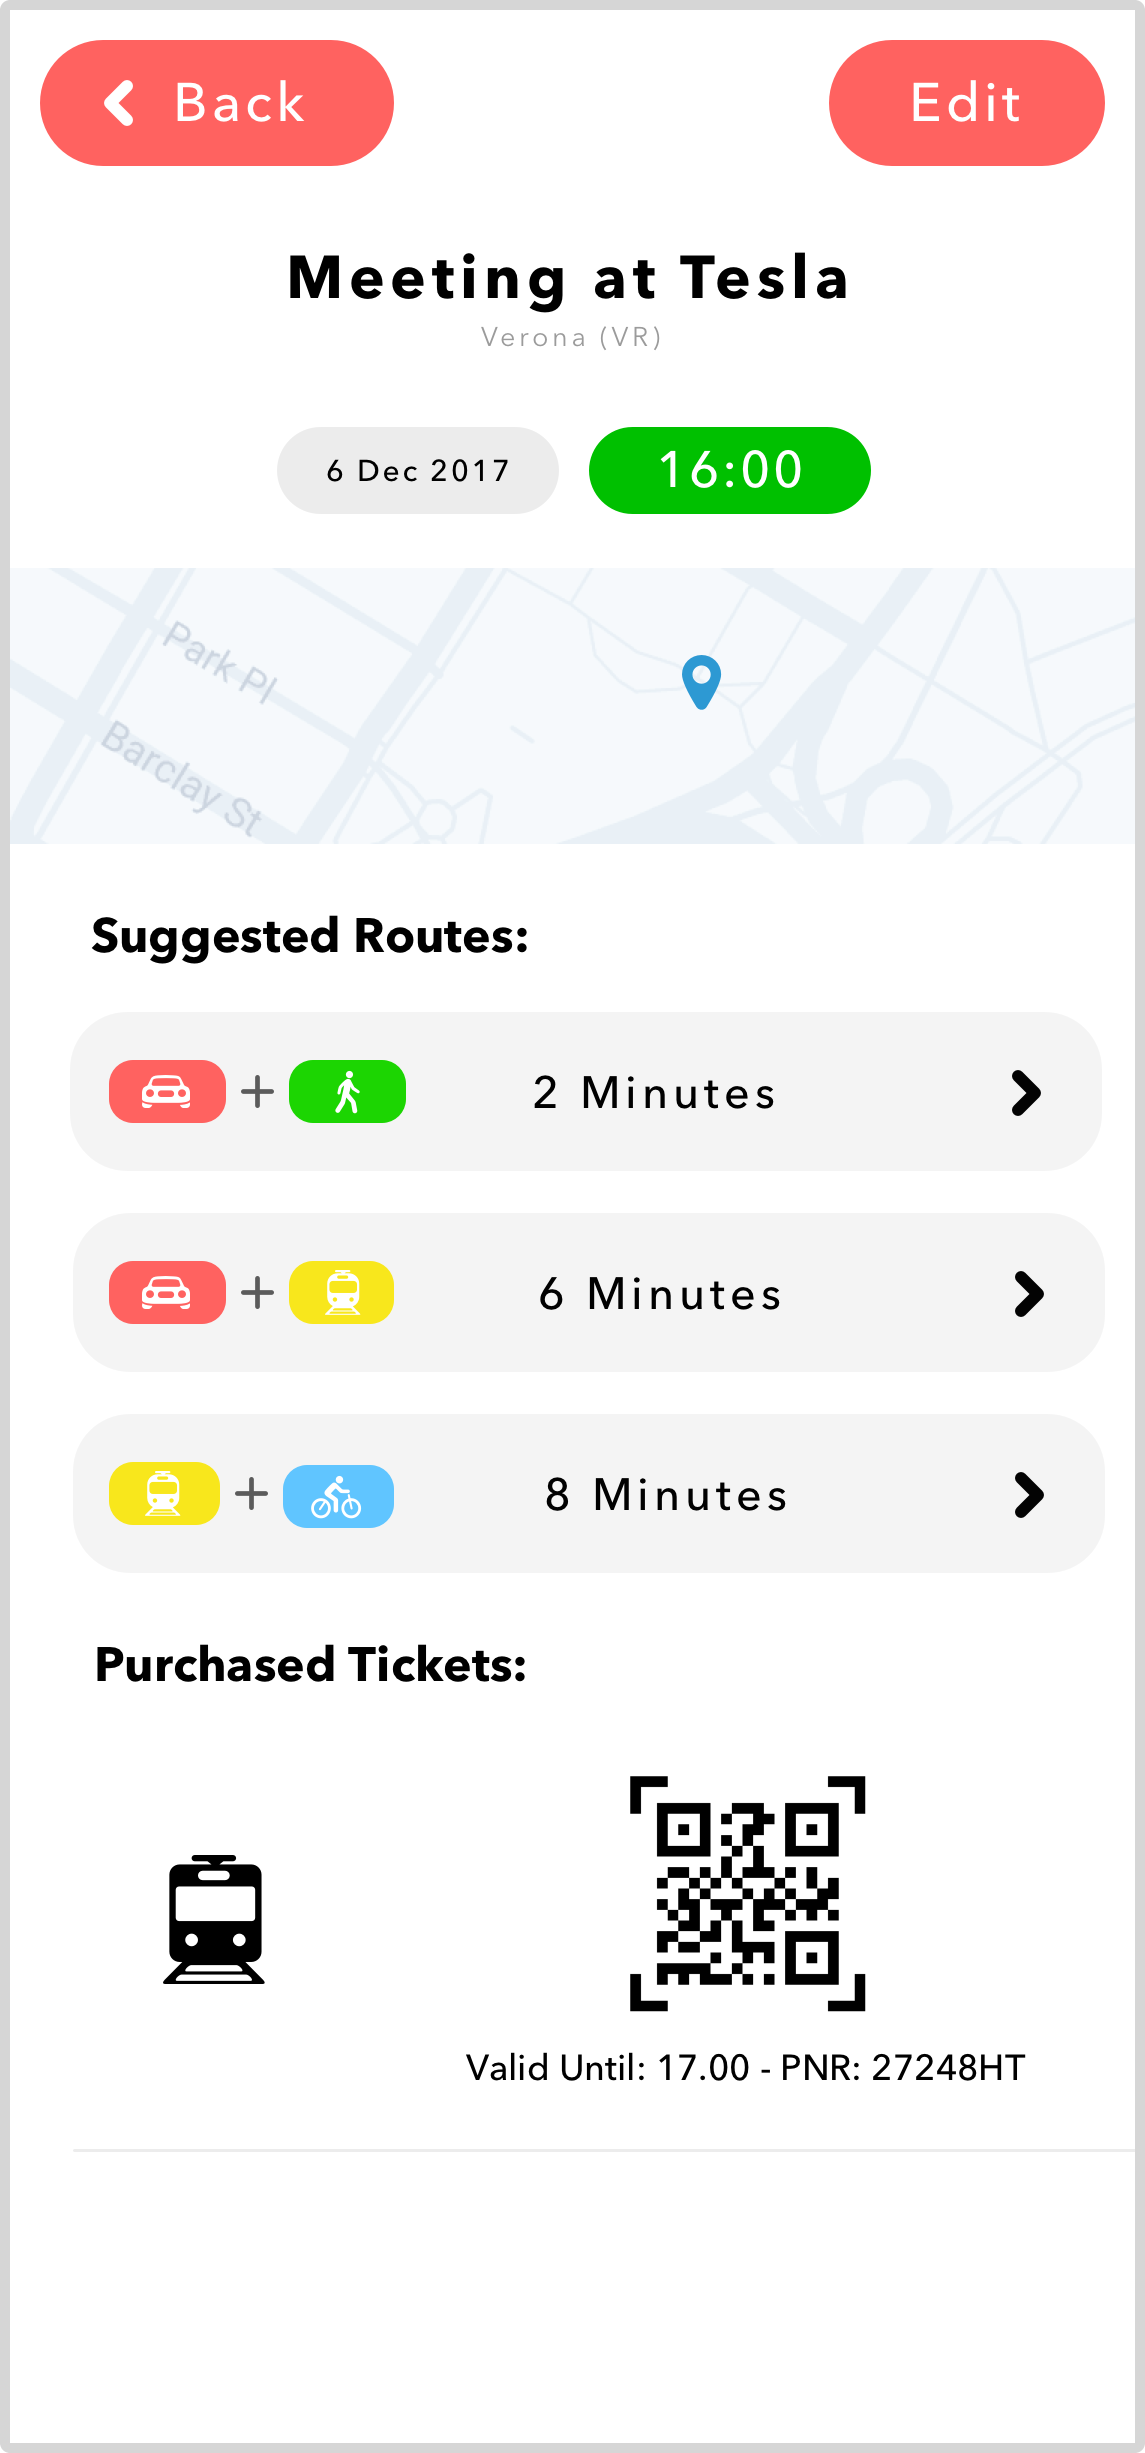
\includegraphics[scale=0.15]{images/Wireframe/5-EventDetail-Tick_wired@3x}
\par\end{center}

When a user buys a ticket it appear in this view which is the main
``Event Detail''. A QR code containing the PNR code of the ticket
is shown.

\pagebreak{}

\paragraph{Add Event}

\vspace*{\bigskipamount}
\begin{center}
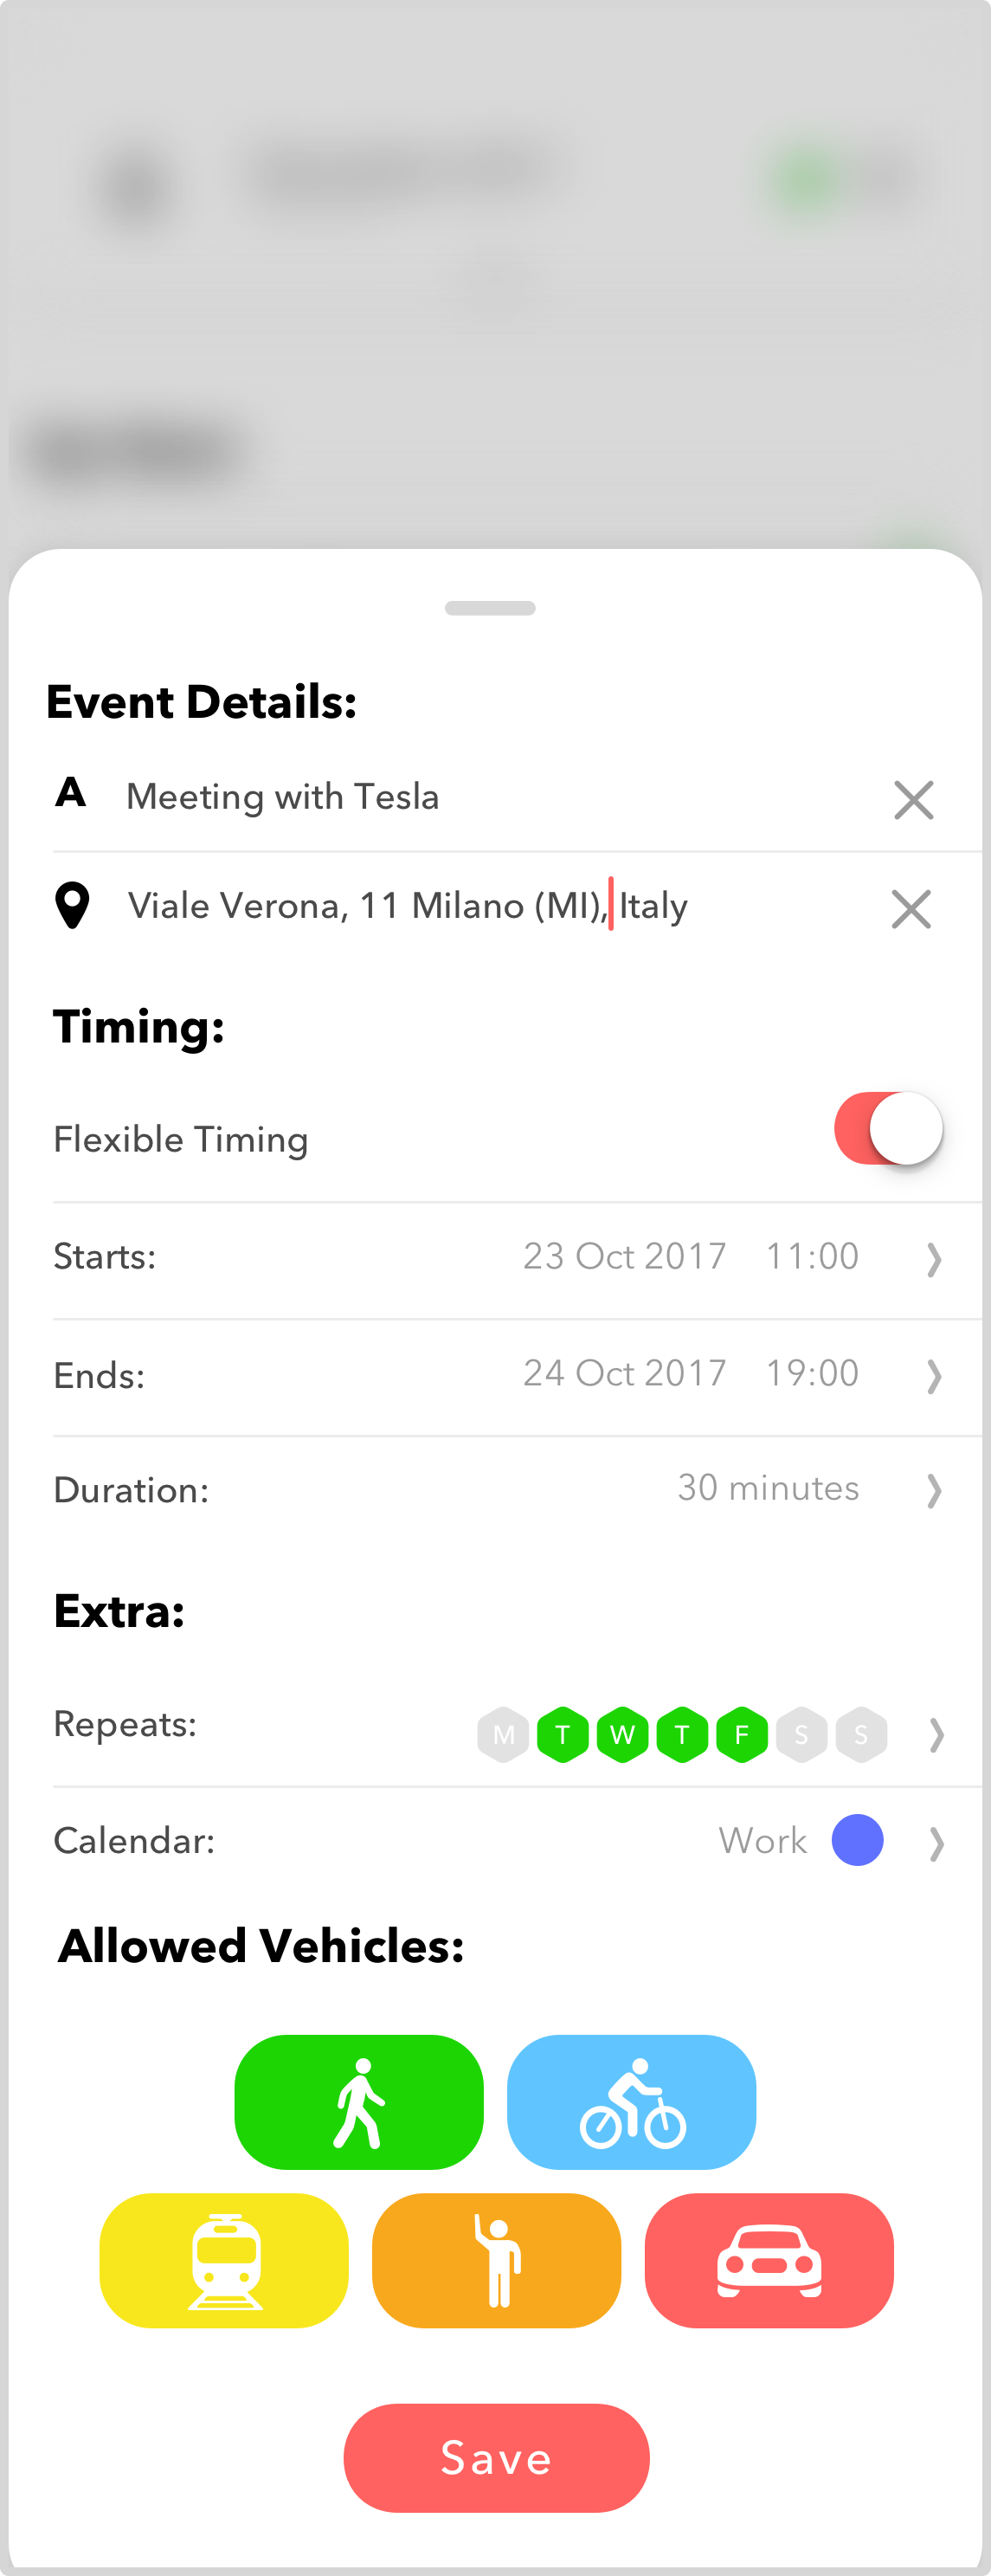
\includegraphics[scale=0.15]{images/Wireframe/7-AddEv_wired@3x}
\par\end{center}

On the main view, once the user taps the add button this pop-up is
shown.

From this area, the person is able to choose:
\begin{itemize}
\item Name of the event
\item Location of the event
\item Start time and end time
\item By toggling the ``Flexible Timing'' switch a new cell called ``Duration''
would appear so that they can just say indicate the how long for this
event will last, given a time window. This feature is useful to set
breaks during the day.
\item Repetition days and a calendar where the event will be saved
\item Vehicles and travel means to compute the best route based on them
\end{itemize}
\pagebreak{}

\paragraph{Add Event / Repetitions}

\vspace*{\bigskipamount}
\begin{center}
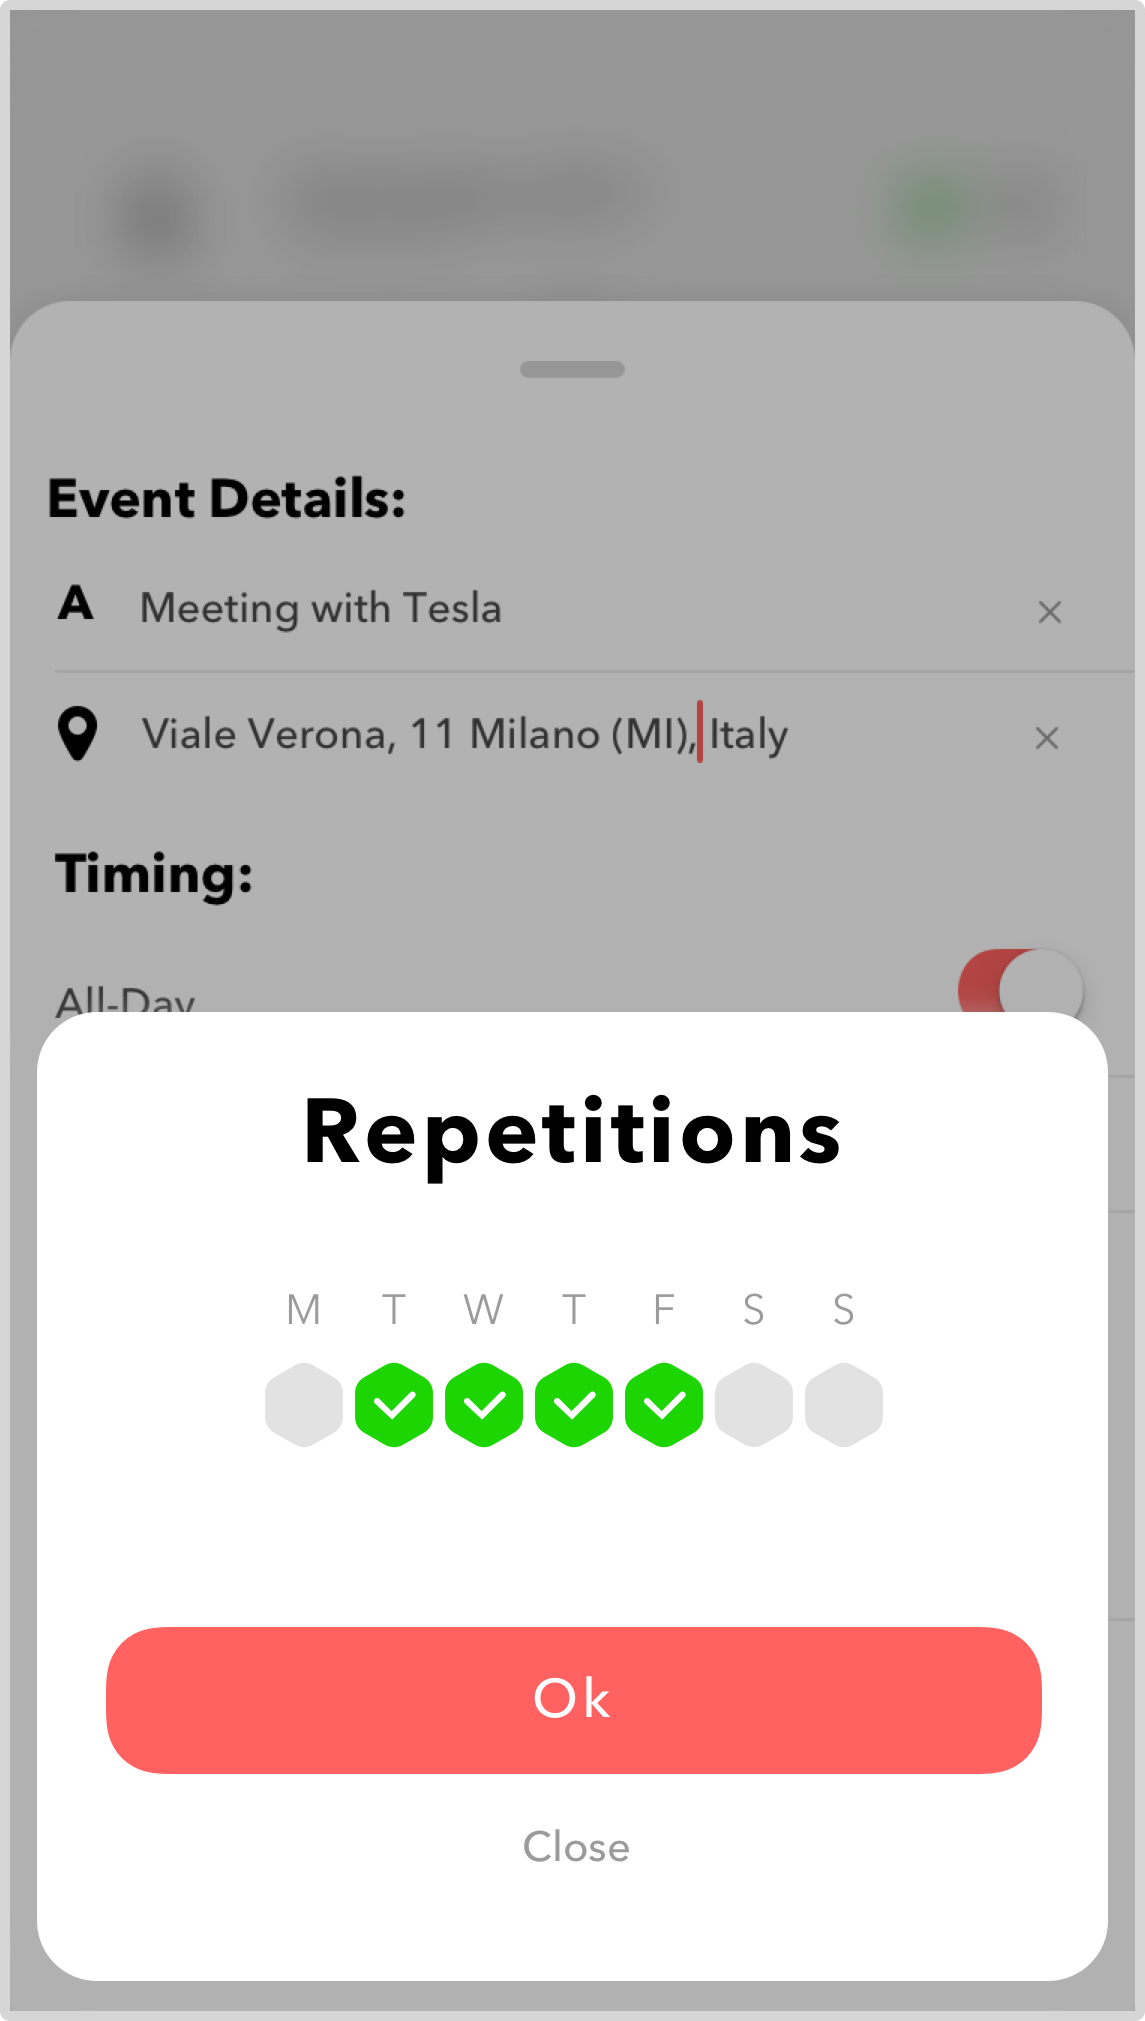
\includegraphics[scale=0.15]{images/Wireframe/8-AddEvent-Repetiti_wired@3x}
\par\end{center}

Here is shown the pop-up that will appear once the user taps on the
``Repeats'' cell from the ``Add Event'' screen.

\pagebreak{}

\paragraph{Add Event / Start Date Time}

\vspace*{\bigskipamount}
\begin{center}
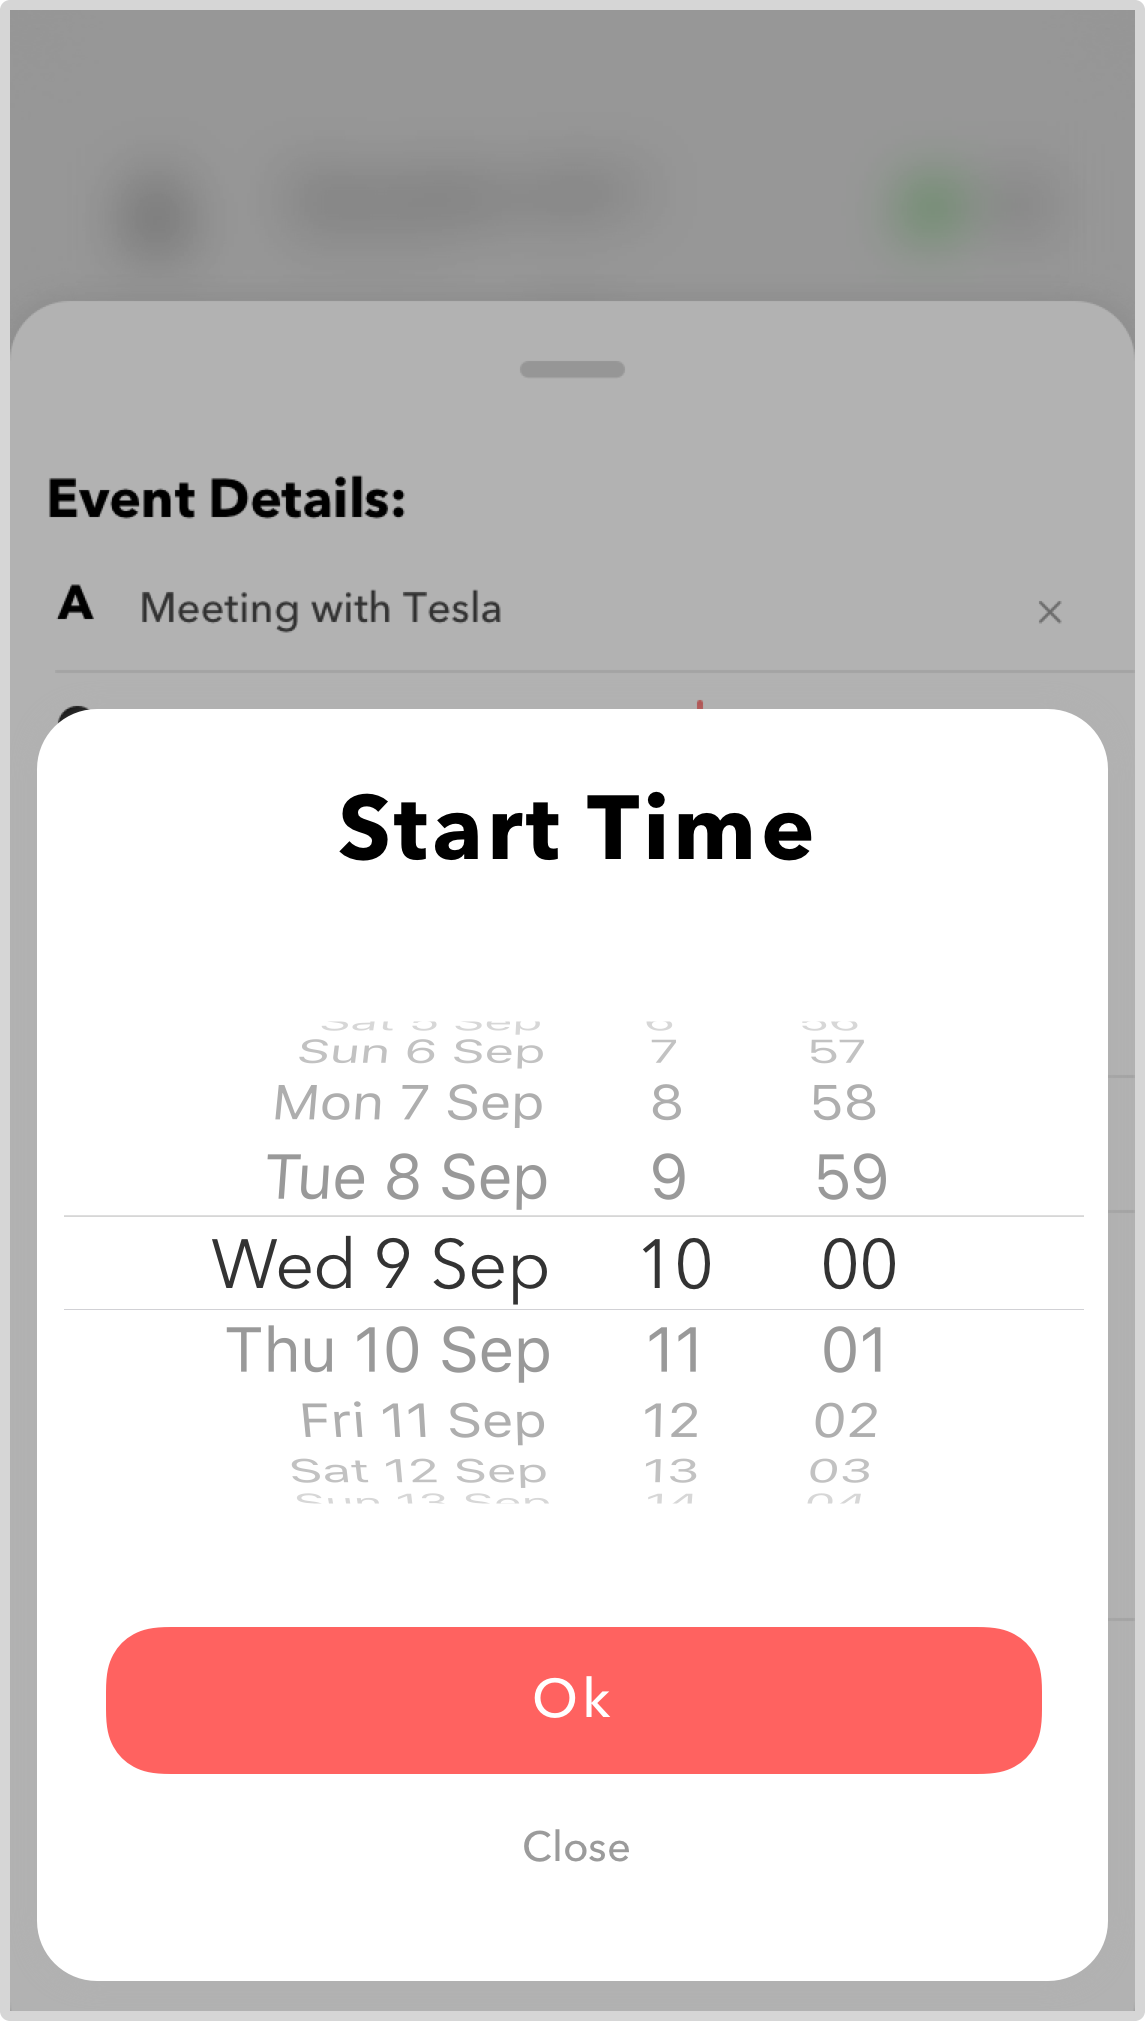
\includegraphics[scale=0.15]{images/Wireframe/9-AddEvent-StartDateT_wired@3x}
\par\end{center}

This is the pop-up that will appear once the user taps on the ``Starts''
cell from the ``Add Event'' screen.

\pagebreak{}

\paragraph{Add Event / End Date Time}

\vspace*{\bigskipamount}
\begin{center}
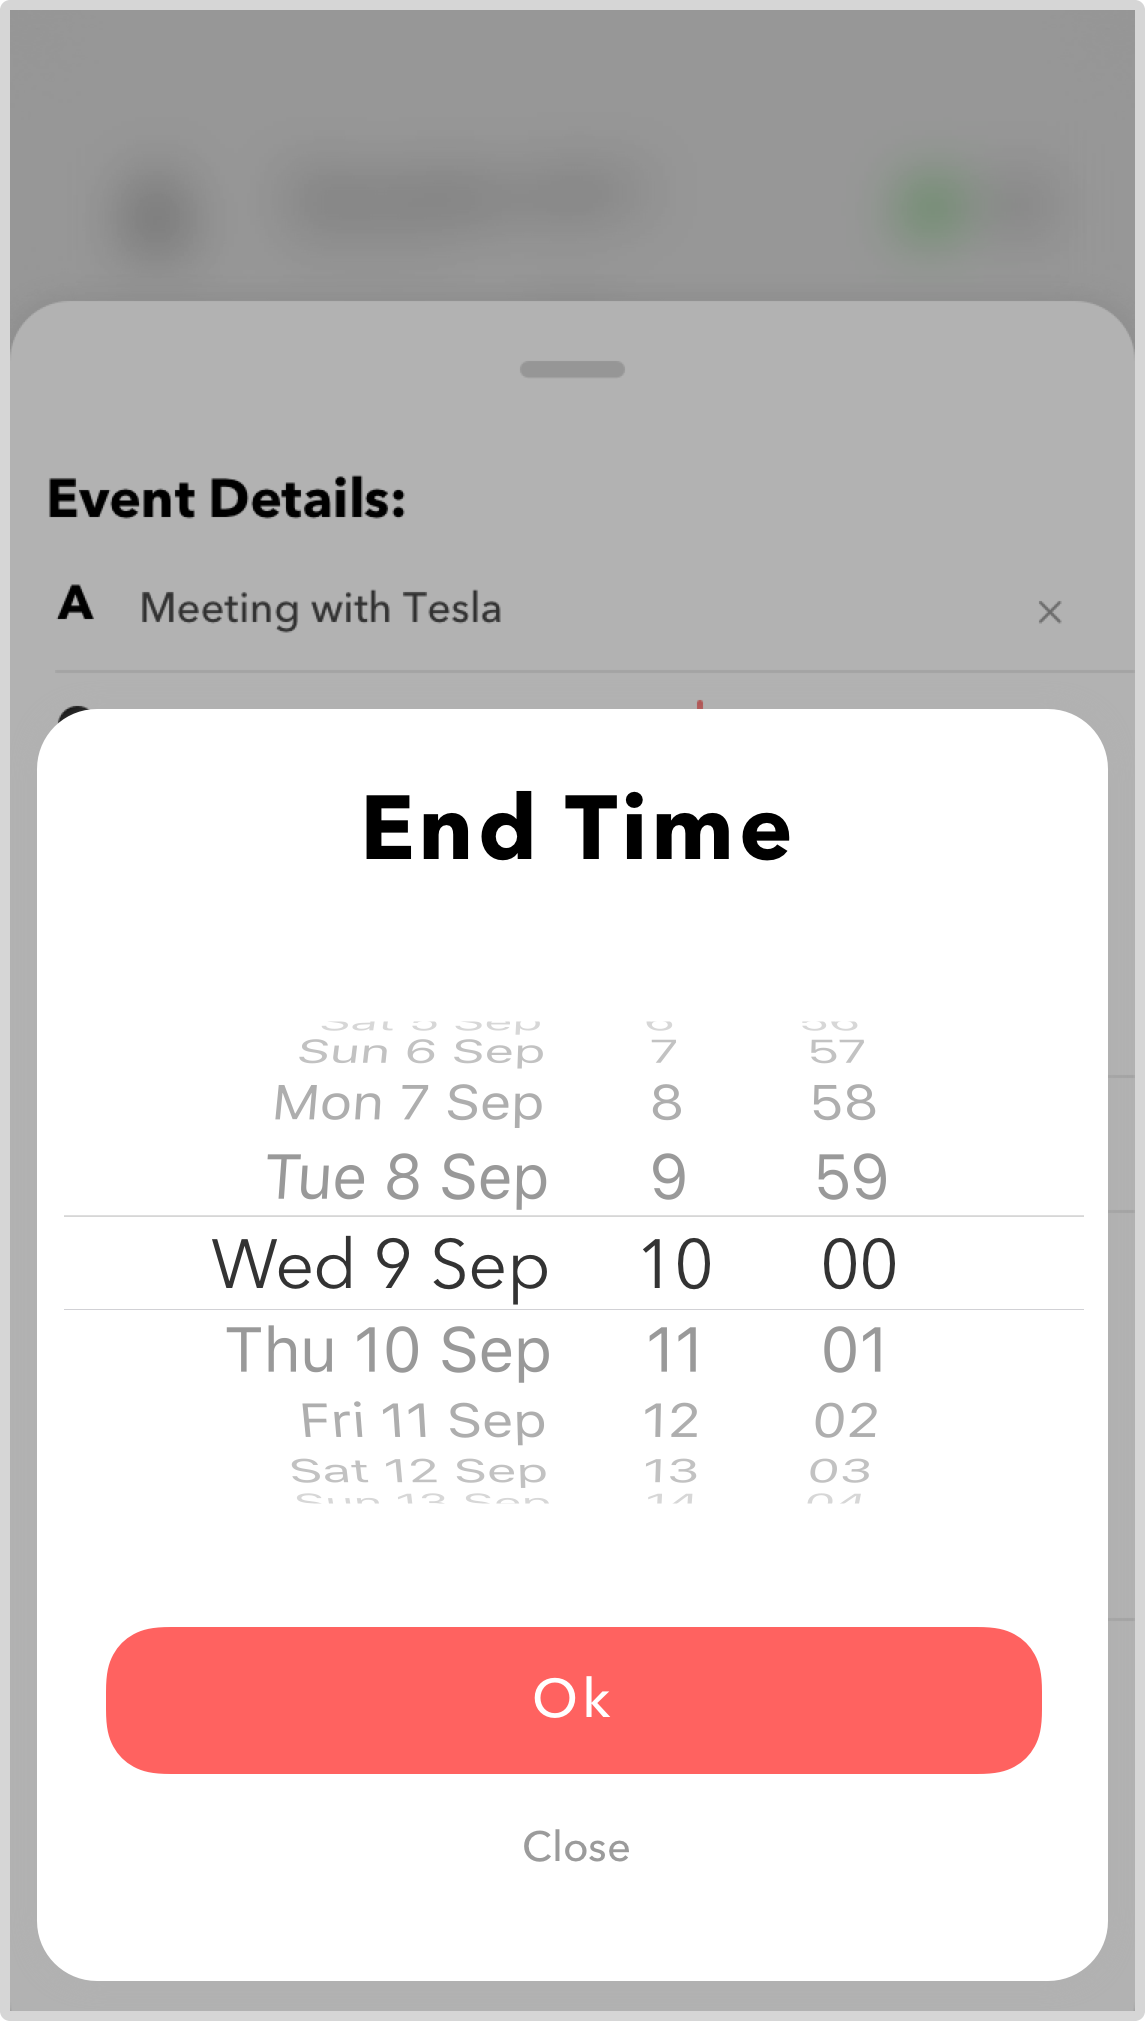
\includegraphics[scale=0.15]{images/Wireframe/10-AddEvent-EndDateT_wired@3x}
\par\end{center}

This is the pop-up that will appear once the user taps on the ``Ends''
cell from the ``Add Event'' screen.

\pagebreak{}

\paragraph{Add Event / Calendar Pick}

\vspace*{\bigskipamount}
\begin{center}
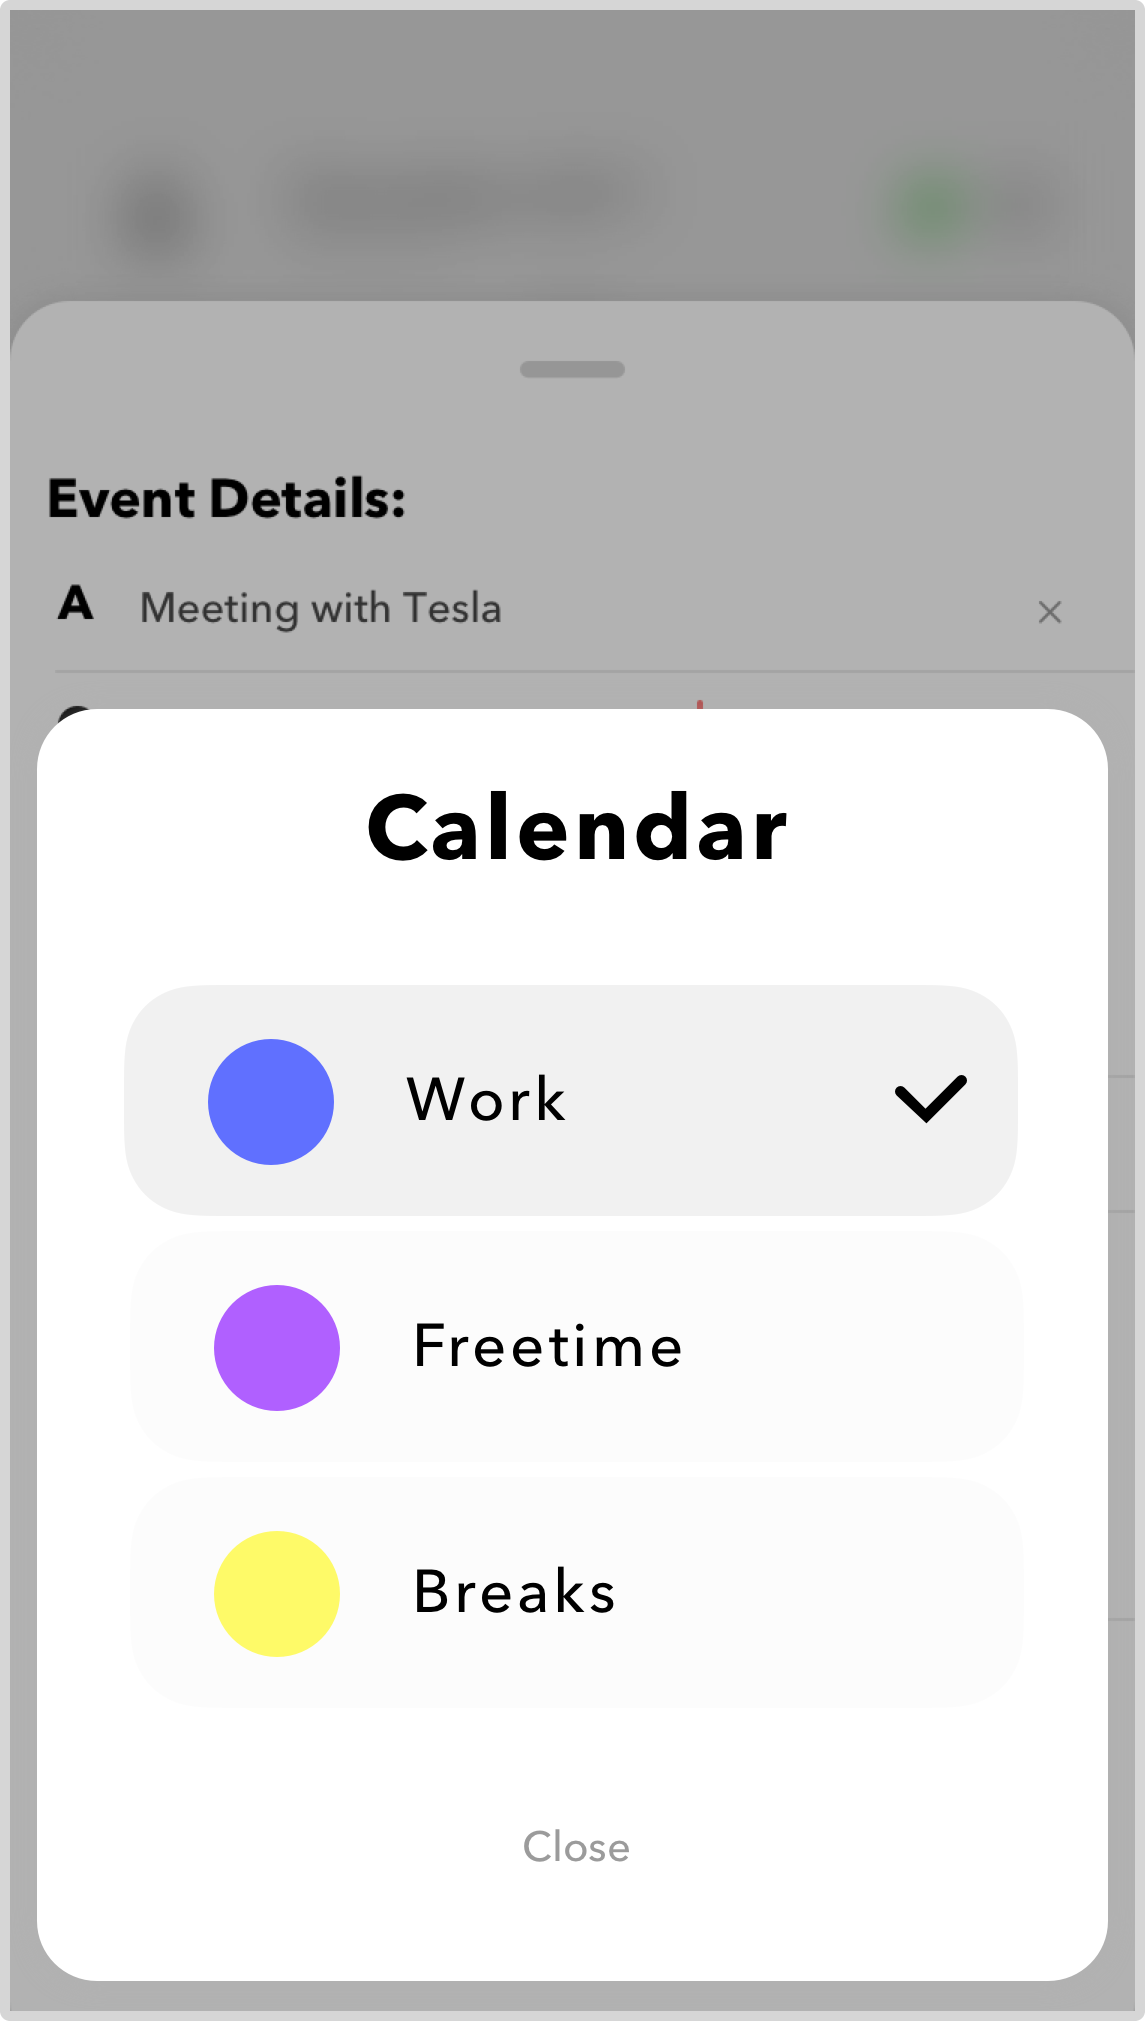
\includegraphics[scale=0.15]{images/Wireframe/11-AddEvent-CalendarP_wired@3x}
\par\end{center}

This is the pop-up that will appear once the user taps on the ``Calendar''
cell from the ``Add Event'' screen.

\pagebreak{}

\paragraph{Map}

\vspace*{\bigskipamount}
\begin{center}
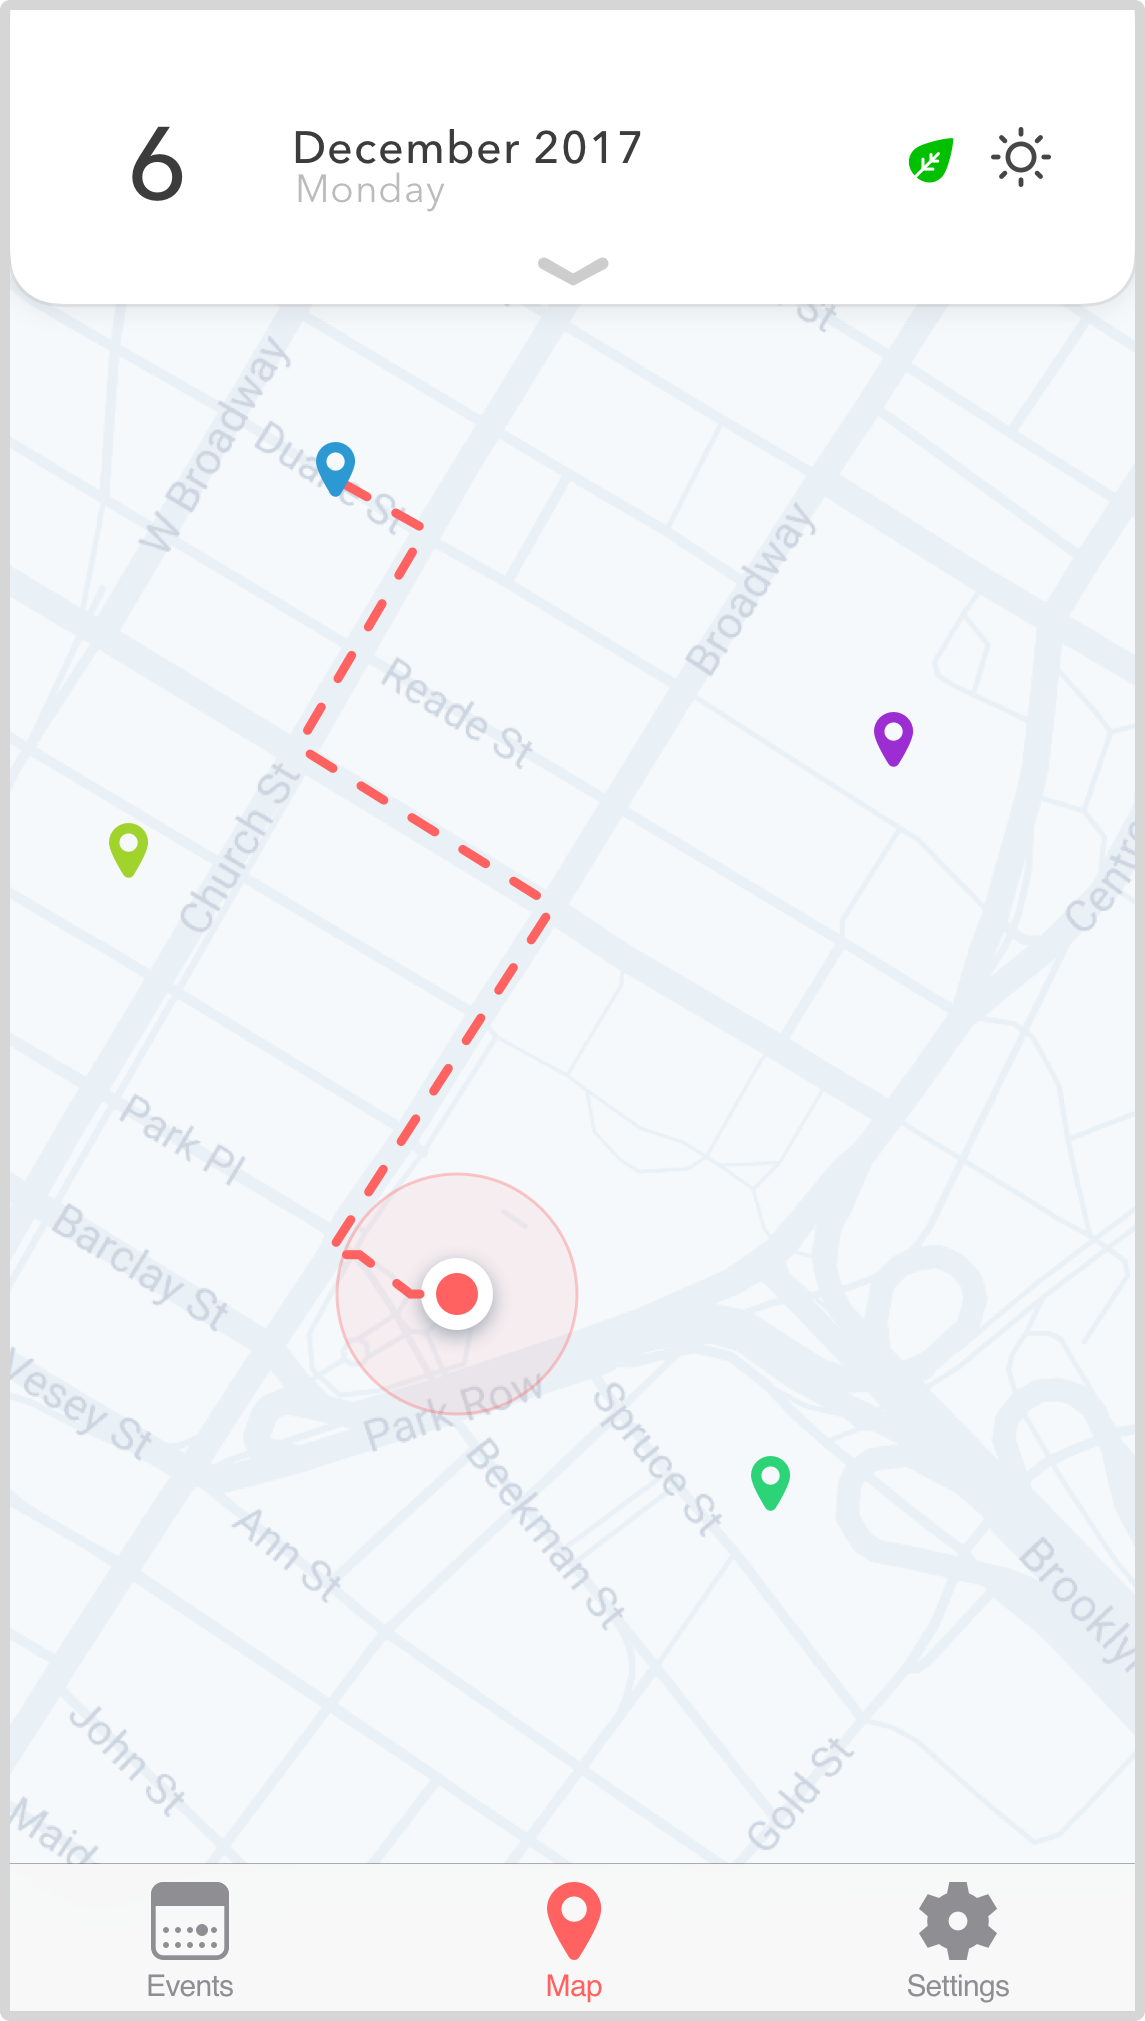
\includegraphics[scale=0.15]{images/Wireframe/12-_wired@3x}\enskip{}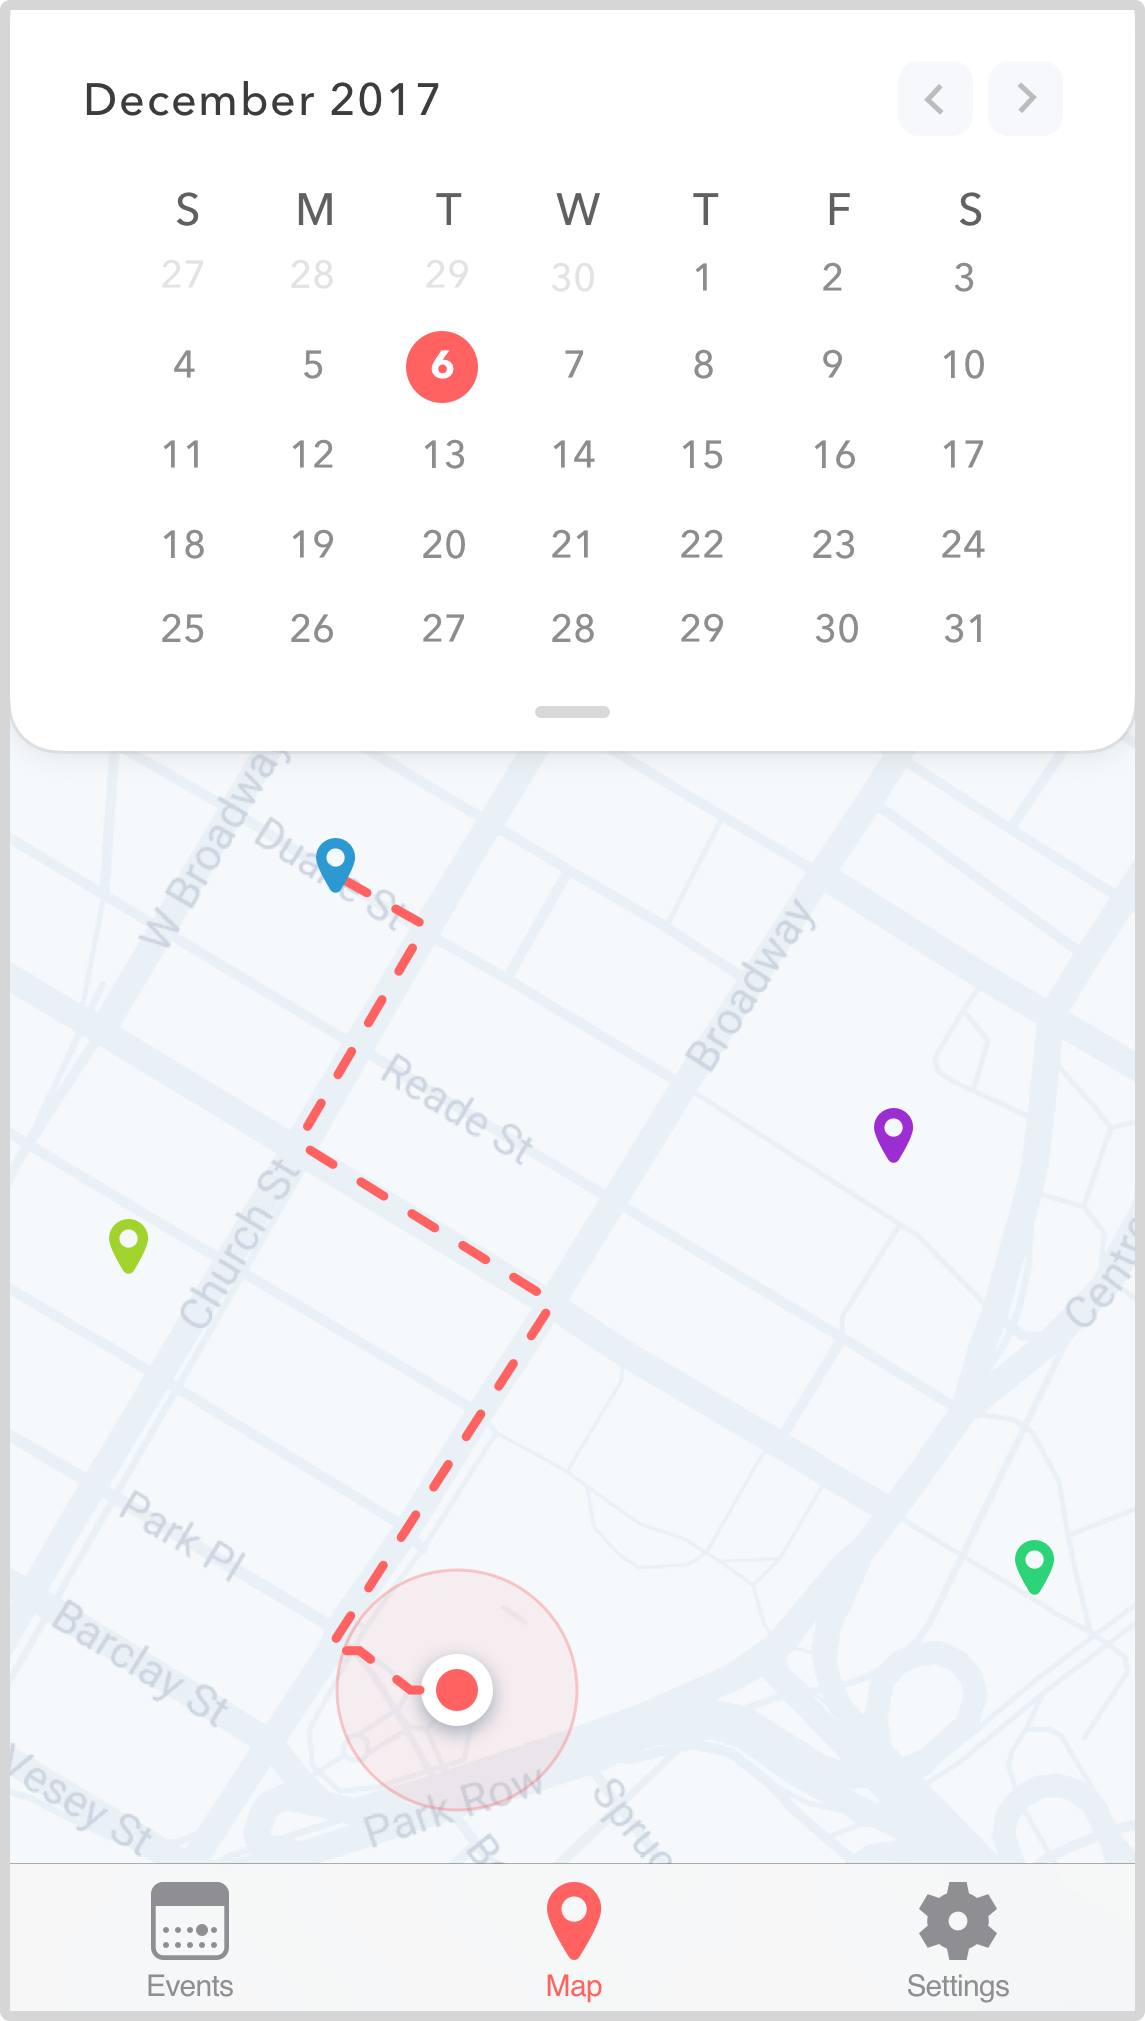
\includegraphics[scale=0.15]{images/Wireframe/13-MapExpan_wired@3x}
\par\end{center}

Swiping right from the main view or by tapping on the bottom icon
the app will present this view.

Here the user can have a look at their daily events on a map. The
screen shows also the suggested route from the actual position to
the first event location.

By pulling down the calendar, the user can change day and have a look
at those specific events.

\pagebreak{}

\paragraph{Settings}

\vspace*{\bigskipamount}
\begin{center}
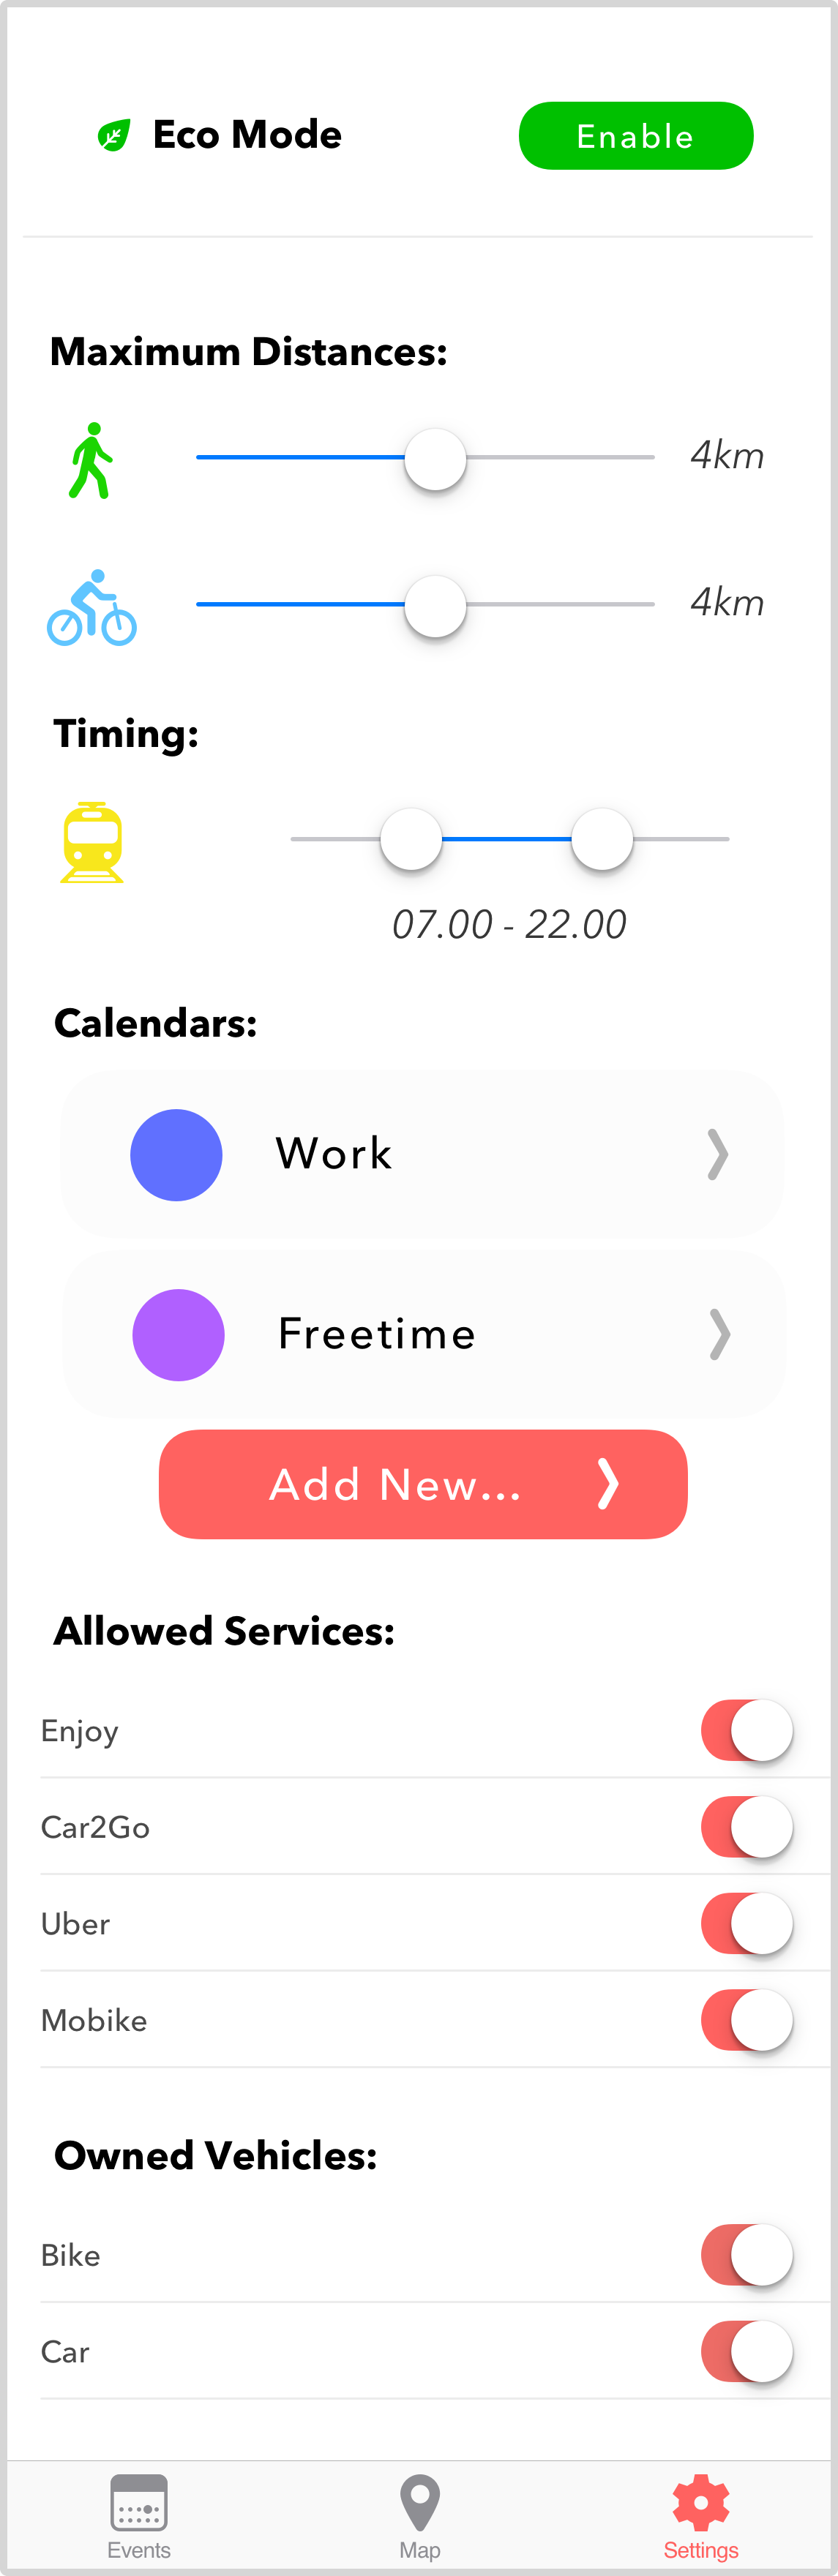
\includegraphics[scale=0.15]{images/Wireframe/14-Setti_wired@3x}
\par\end{center}

Swiping right from the map view or by tapping on the bottom icon the
app will present this view.

Here we can find five sections:
\begin{enumerate}
\item \textbf{Eco Mode:} By enabling it the system will differently weight
routes that require fossil fuel based vehicles
\item \textbf{Maximum Distances:} User is allowed to set a maximum amount
of distance by walk or bike so that the system will re arrange its
calculations based on this new values.
\item \textbf{Timing:} Here the user can set the time window where transits
will be available
\item \textbf{Calendars:} In this section the user can edit his existing
calendars or create a new one by tapping ``Add New...'' button
\item \textbf{Allowed Services:} Here the user can just activate or disable
vehicle-sharing services (such as Enjoy or Mobike) so that the app
will not consider them on paths calculations.
\end{enumerate}
\pagebreak{}

\paragraph{Settings / Add Calendar}

\vspace*{\bigskipamount}
\begin{center}
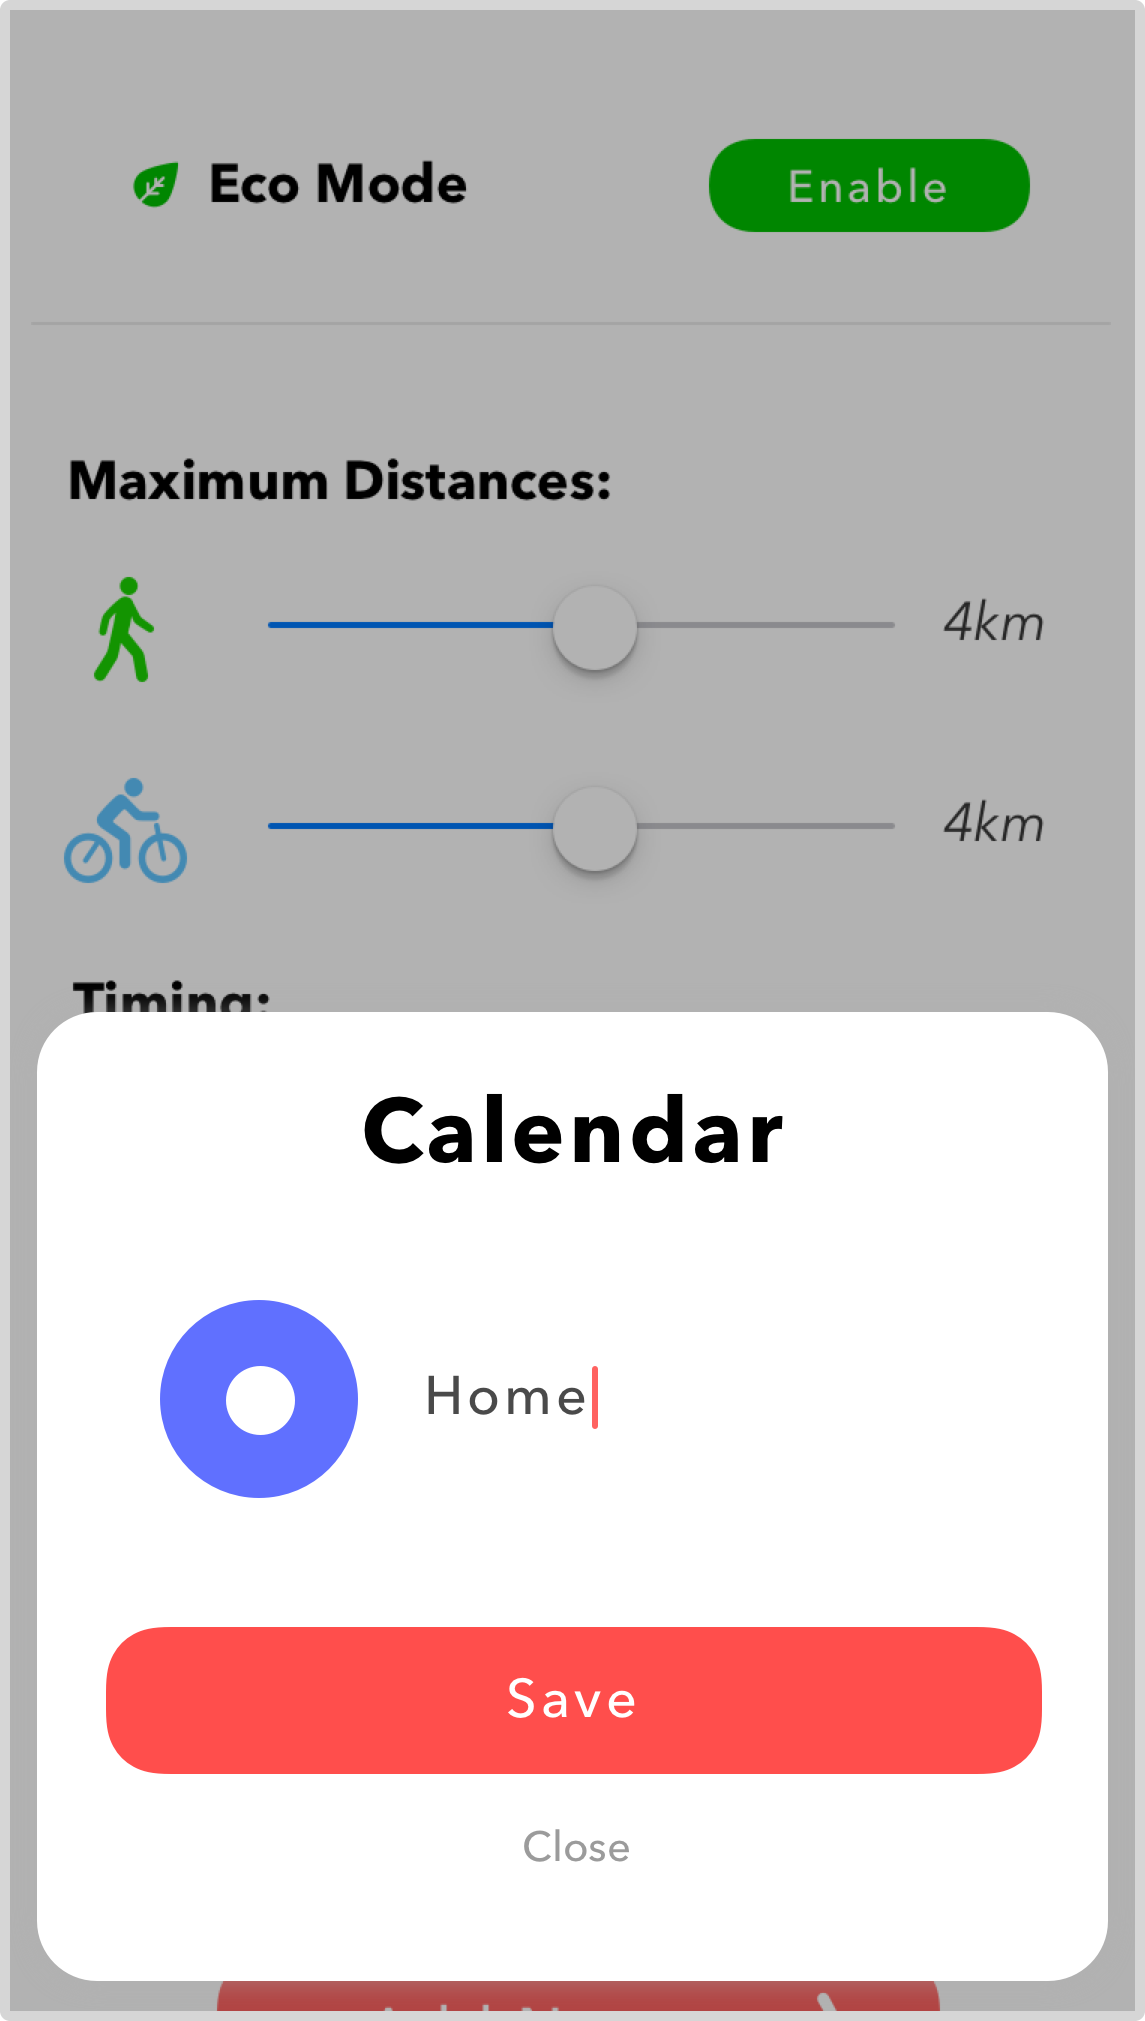
\includegraphics[scale=0.15]{images/Wireframe/15-Settings-AddCalen_wired@3x}
\par\end{center}

This is the view that will be shown when the user wants to add a new
calendar.

\pagebreak{}

\paragraph{Settings / Add Calendar / Color}

\vspace*{\bigskipamount}
\begin{center}
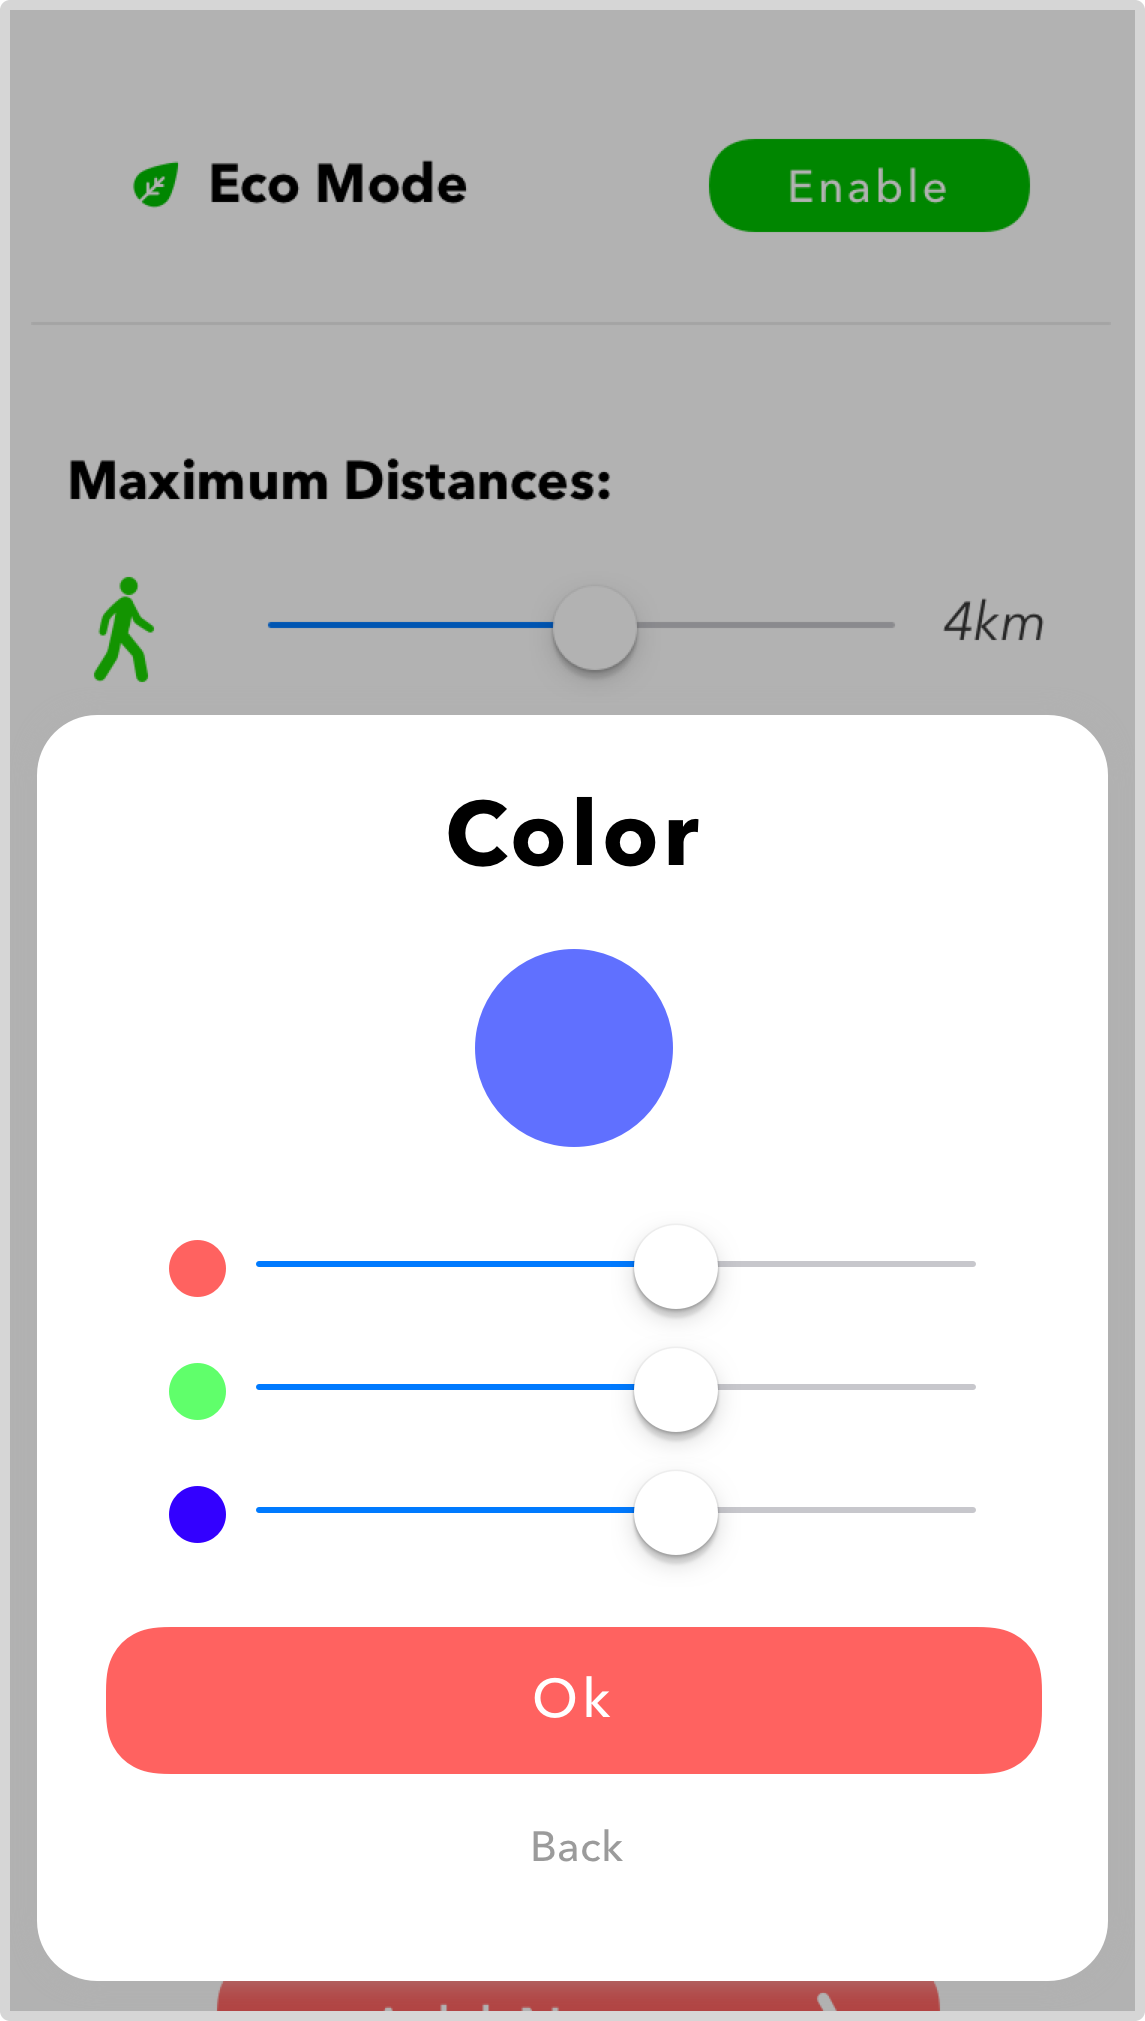
\includegraphics[scale=0.15]{images/Wireframe/16-Settings-EditCalendarCo_wired@3x}
\par\end{center}

This is the view where the user is allowed to edit the color of an
existing or new calendar just by adjusting the RGB Sliders.

\pagebreak{}

\subsubsection{Hardware Interfaces }

The system will require, in order to work properly, one or more dedicated
servers in which the server management software will run.

\subsubsection{Software Interfaces }

The system will need:
\begin{itemize}
\item A server database where it will store user data like calendars, events
and preferences.
\item A client database where it will store user data on device so that
the app will work offline too.
\item The App that will be installed on the users's smartphones.
\end{itemize}

\subsubsection{Communication Interfaces}

In order to establish a communication between the app and the server,
there will be the need to build an API that lets the app to store
and/or retrieve data from the database (located server-side). The
connection will be created though the HTTPS protocol and the data
will be exchanged with a JSON encoding.

\pagebreak{}

\subsection{Functional Requirements}

\subsubsection{{[}G0{]} Allow people to use the app without a login function}
\begin{itemize}
\item {[}R1{]} When the app is lunched for the first time, the system recognizes
the new users and create a record of their data to be locally updated
on the phone
\end{itemize}
%
\begin{itemize}
\item {[}D1{]} App data are stored remotely and retrieved by multiple devices
\end{itemize}

\subsubsection{{[}G1{]} Allow people to view the daily schedule with coming up events
at the top}
\begin{itemize}
\item {[}R2{]} The system must be able to provide the list of daily events
scheduled by the user
\item {[}R3{]} The events must be divided between ``Up coming'' and ``Later
on''
\item {[}R4{]} Information of event's description, calendar saved and time
must always be shown, while the location of the event is optional
\item {[}R5{]} Button add event must always be visible
\end{itemize}
%
\begin{itemize}
\item {[}D2{]} Up coming events' section needs to contain appointments planned
to happen 2h before
\end{itemize}

\subsubsection{{[}G2{]} Allow people to view previous events}
\begin{itemize}
\item {[}R6{]} A calendar screen must be shown
\item {[}R7{]} Information of event's description, calendar saved and time
must always be shown, while the location of the event is optional
\item {[}R8{]} Button add event must always be visible
\end{itemize}
%
\begin{itemize}
\item {[}D3{]} Transportation information are not shown for the past events
\end{itemize}

\subsubsection{{[}G3{]} Allow people to view the detail of each event}
\begin{itemize}
\item {[}R9{]} ETA and trip information must be provided
\item {[}R10{]} Tickets services must be shown
\item {[}R11{]} Different suggested routes can be explored, if available
\item {[}R12{]} The system must provide a way to buy tickets or book a sharing
service vehicle
\item {[}R13{]} The system must show the purchased ticket
\item {[}R14{]} The paths color in the map changes accordingly to the means
of transportation
\end{itemize}
%
\begin{itemize}
\item {[}D4{]} Indications on the ETA, calculated mean of transportation
and time-to-leave are calculated on the current approximative position
\item {[}D5{]} User's position is retrieved using GPS system
\item {[}D6{]} Position is re-calculated every 2 hours, or when a significant
change in GPS position is discovered
\item {[}D7{]} The map can be browsed by the user
\item {[}D8{]} The localization service is available and functionally working
\item {[}D9{]} The map service is reliable
\end{itemize}

\subsubsection{{[}G4{]} Allow the users to create an event}
\begin{itemize}
\item {[}R15{]} Information of event's description, calendar saved and time
must always be provided, while the location of the event is optional
\item {[}R16{]} The system must ask for the description and the location
of the appointment
\item {[}R17{]} The system must ask whether the event should be time-flexible.
In this case it must require a time window and how long the appointment
will last
\item {[}R18{]} Button for repeating an event weekly must be shown
\item {[}R19{]} Button for choosing the calendar in which the event will
be saved must be shown
\item {[}R20{]} A multiple choice list of available means of transportation
must be included
\end{itemize}
%
\begin{itemize}
\item {[}D10{]} The button to choose the calendar is, by default, the last
calendar chosen, or the first calendar if the user has never added
an event
\item {[}D11{]} While creating an event, the system must take into account
whether the eco mode has been turned on
\item {[}D17{]} Each event belongs to only one calendar
\item {[}D18{]} The user won't insert overlapping events
\end{itemize}

\subsubsection{{[}G5{]} Allow people to see daily events on a map}
\begin{itemize}
\item {[}R21{]} All the events must be shown on a interactive map
\item {[}R22{]} The map must show a path to the next event 
\end{itemize}
%
\begin{itemize}
\item {[}D12{]} The map can be browsed by the user
\item {[}D5{]} User's position is retrieved using GPS system
\item {[}D9{]} The map service is reliable
\end{itemize}

\subsubsection{{[}G6{]} Allow the user to set preferences}
\begin{itemize}
\item {[}R23{]} The system must provide of a way to change the maximum distance
that could be traveled by bike or walk
\item {[}R24{]} The system must provide a time window in which public transits
can be taken
\item {[}R25{]} All the available calendars must be shown
\item {[}R26{]} The system must allow to toggle the available external sharing
services
\end{itemize}
%
\begin{itemize}
\item {[}D13{]} Every preference agrees with the actual record saved in
the database 
\item {[}D14{]} Allowed services have been preinstalled
\end{itemize}

\subsubsection{{[}G7{]} Allow the users to create calendars}
\begin{itemize}
\item {[}R27{]} The app should allow the user to add a new calendar
\item {[}R28{]} The system allows to change the name of a calendar and eventually
its color
\end{itemize}
%
\begin{itemize}
\item {[}D15{]} The user has always at least one calendar
\item {[}D16{]} Each calendar belongs to only one user
\end{itemize}

\subsubsection{{[}G8{]} Notify the user that it's time to leave for the appointment}
\begin{itemize}
\item {[}R29{]} The app must send a notification when it's time to leave
for the appointment.
\item {[}R30{]} The system must take into account the means of transportation
that the user has selected
\end{itemize}
%
\begin{itemize}
\item {[}D5{]} User's position is retrieved using GPS system
\end{itemize}
\pagebreak{}

\subsection{Scenarios}

\subsubsection{Scenario 1}

Mike was invited to John's Party in Los Angeles and he really wants
to go there. Unfortunately he has a lot of memory problems... That's
the reason why John told him to use Travlendar+.

Mike picked up his smartphone and installed it, added the event details
on the main calendar and saved!

Later he received a notification that it was time to leave and so
he could arrive on time at his friend's birthday.

\subsubsection{Scenario 2}

Steve is always too busy and he participates to a huge variety of
events so he needs to create new calendars in which he can store them.
He also cares a lot on tidiness he wants his calendars have great
and appealing colors in order to focus on his events in a better way.

\subsubsection{Scenario 3}

Benedetto is a convinced environmentalist. He wants to make the world
a better place by reducing carbon emissions. For this reason he downloaded
and added all his events in Travlendar+. He then enabled ``Eco Mode''
and now he can really help the environment.

\subsubsection{Scenario 4}

Filippo is a man who doesn't like to walk and neither use a bike therefore
he wants to minimize his effort to reach an event.

He now installed Travlendar+ on his smartphone and set ``Maximum
Distance'' to the minimum value for bike and walk, so he now doesn't
need to struggle to reach an appointment.

\subsubsection{Scenario 5}

Giovanni likes to travel a lot, for this reason he started using this
app. 

He likes a lot to reach locations using public transport or rides,
but he is under age to be allowed to use car sharing providers so
he just disabled suggestions for car sharing services right on the
app and now he is happy more than ever.

\subsection{Definition of use cases}

\subsubsection{CreateCalendar}

Allow the user to create a new calendar with a name and a color chosen
by the user

\vspace*{\bigskipamount}

\begin{tabular}{|>{\raggedright}m{0.2\textwidth}|>{\raggedright}m{0.8\textwidth}|}
\hline 
Name & CreateCalendar\tabularnewline
\hline 
Actors & User\tabularnewline
\hline 
Goals & {[}G7{]}\tabularnewline
\hline 
Input conditions & None\tabularnewline
\hline 
Flow of Events & \begin{enumerate}
\item The users swipes to reach the settings tab
\item Under the Calendar section, the user choses ``Add new''
\item A pop-up is shown with a name and color input
\item The user chooses the calendar name and its color
\item The system records the new calendar in the database
\end{enumerate}
\tabularnewline
\hline 
Output conditions & The calendar is saved in the database\tabularnewline
\hline 
Exceptions & None\tabularnewline
\hline 
\end{tabular}

\pagebreak{}

\subsubsection{AddStandardEvent}

Allow the user to insert an event in the calendar

\vspace*{\bigskipamount}

\begin{tabular}{|>{\raggedright}m{0.2\textwidth}|>{\raggedright}m{0.8\textwidth}|}
\hline 
Name & AddStandardEvent\tabularnewline
\hline 
Actors & User\tabularnewline
\hline 
Goals & {[}G4{]}\tabularnewline
\hline 
Input conditions & None\tabularnewline
\hline 
Flow of Events & \begin{enumerate}
\item The user selects ``Add event'' from the ``schedule'' view
\item A pop-up is shown with a form to fill out
\item The user chooses the location and a description
\item The user selects the starting and ending date-time
\item Eventual repetitions during the week and type of calendar are chosen
\item Preferred means of transportation are selected
\item The system checks if the appointment can be reached in time with the
user's preferred vehicles
\item The system rearrange flexible events in order to fit the schedule
\item Event's details are shown
\end{enumerate}
\tabularnewline
\hline 
Output conditions & \begin{itemize}
\item The event is added to the calendar
\item Flexible events are rearranged to fit the schedule
\end{itemize}
\tabularnewline
\hline 
Exceptions & Users are notified immediately with a warning if their event will
not be reached on time\tabularnewline
\hline 
\end{tabular}

\pagebreak{}

\subsubsection{AddFlexibleEvent}

Allow the user to insert a flexible event in the calendar

\vspace*{\bigskipamount}

\begin{tabular}{|>{\raggedright}m{0.2\textwidth}|>{\raggedright}m{0.8\textwidth}|}
\hline 
Name & AddFlexibleEvent\tabularnewline
\hline 
Actors & User\tabularnewline
\hline 
Goals & {[}G4{]}, {[}G4.3{]}\tabularnewline
\hline 
Input conditions & None\tabularnewline
\hline 
Flow of Events & \begin{enumerate}
\item The user selects ``Add event'' from the ``schedule'' view
\item A pop-up is shown with a form to fill out
\item The user choose the location and a description
\item The user toggle the switch for a Flexible Event
\item The user selects the starting and ending date-time window
\item The user choose the duration of the event
\item Eventual repetitions during the week and type of calendar are chosen
\item Preferred means of transportation are selected
\item The system checks if the appointment can be reached in time with the
user's preferred vehicles
\item The system rearrange this and other flexible events in order to fit
the schedule
\item Event's details are shown
\end{enumerate}
\tabularnewline
\hline 
Output conditions & \begin{itemize}
\item The event is added to the calendar
\item Flexible events are rearranged to fit the schedule
\end{itemize}
\tabularnewline
\hline 
Exceptions & Users are notified immediately with a warning if their event will
not be reached on time\tabularnewline
\hline 
\end{tabular}

\pagebreak{}

\subsubsection{EditPreferences}

Allow the users to edit their settings: preferred vehicles (cars,
bikes, public transportation, trains, sharing services), depending
on the weather, if help lowering carbon emission or not, and specify
a preferred lunch time

\vspace*{\bigskipamount}

\begin{tabular}{|>{\raggedright}m{0.2\textwidth}|>{\raggedright}m{0.8\textwidth}|}
\hline 
Name & EditPreferences\tabularnewline
\hline 
Actors & User\tabularnewline
\hline 
Goals & {[}G6{]}\tabularnewline
\hline 
Input conditions & None\tabularnewline
\hline 
Flow of Events & \begin{enumerate}
\item The user selects the ``Settings'' tab
\item A window with all the available settings is displayed
\item The user chooses preferences
\item The settings are automatically saved
\end{enumerate}
\tabularnewline
\hline 
Output conditions & The preferences are saved into user's profile\tabularnewline
\hline 
Exceptions & None\tabularnewline
\hline 
\end{tabular}

\pagebreak{}

\subsubsection{BuyTickets}

Allow the user to buy public transportation tickets directly from
the application.

\vspace*{\bigskipamount}

\begin{tabular}{|>{\raggedright}m{0.2\textwidth}|>{\raggedright}m{0.8\textwidth}|}
\hline 
Name & BuyTickets\tabularnewline
\hline 
Actors & User\tabularnewline
\hline 
Goals & {[}G3.2.1{]}\tabularnewline
\hline 
Input conditions & \begin{itemize}
\item The event has already been created
\item The user is seeing a suggested route
\item The suggested route has a public transit option
\end{itemize}
\tabularnewline
\hline 
Flow of Events & \begin{enumerate}
\item The user taps on the ``Purchase ticket'' button
\item The text message app is displayed in foreground with a predefined
text and the local transit company number as receiver
\item The user sends the text message
\item The user receives a reply from the local transit company with a PNR
code
\item The text message sent from the local transit company is read by the
application
\end{enumerate}
\tabularnewline
\hline 
Output conditions & The ticket is recorded in the database\tabularnewline
\hline 
Exceptions & The purchased is aborted if the user doesn't have enough credit on
the phone\tabularnewline
\hline 
\end{tabular}

\pagebreak{}

\subsubsection{NotifyUser}

When an upcoming event is detected, the system sends a notification
to the user

\vspace*{\bigskipamount}

\begin{tabular}{|>{\raggedright}m{0.2\textwidth}|>{\raggedright}m{0.8\textwidth}|}
\hline 
Name & NotifyUser\tabularnewline
\hline 
Actors & User, System\tabularnewline
\hline 
Goals & {[}G8{]}\tabularnewline
\hline 
Input Conditions & The event was created by the user\tabularnewline
\hline 
Flow of Events & \begin{enumerate}
\item The system checks the current user position
\item The system checks wether there is an upcoming event
\item When an event is found the system plans the travel
\item If it's time to go, the system sends the notification to the user
\end{enumerate}
\tabularnewline
\hline 
Output conditions & The user is now aware to leave to the appointment\tabularnewline
\hline 
Exceptions & \begin{itemize}
\item The system waits for the next cycle if there is no upcoming event
\item The system waits for the next cycle if it's too early to leave to
the appointment
\end{itemize}
\tabularnewline
\hline 
\end{tabular}

\pagebreak{}

\subsection{Sequence Diagrams}

\subsubsection{AddStandardOrFlexibleEvent}
\begin{center}
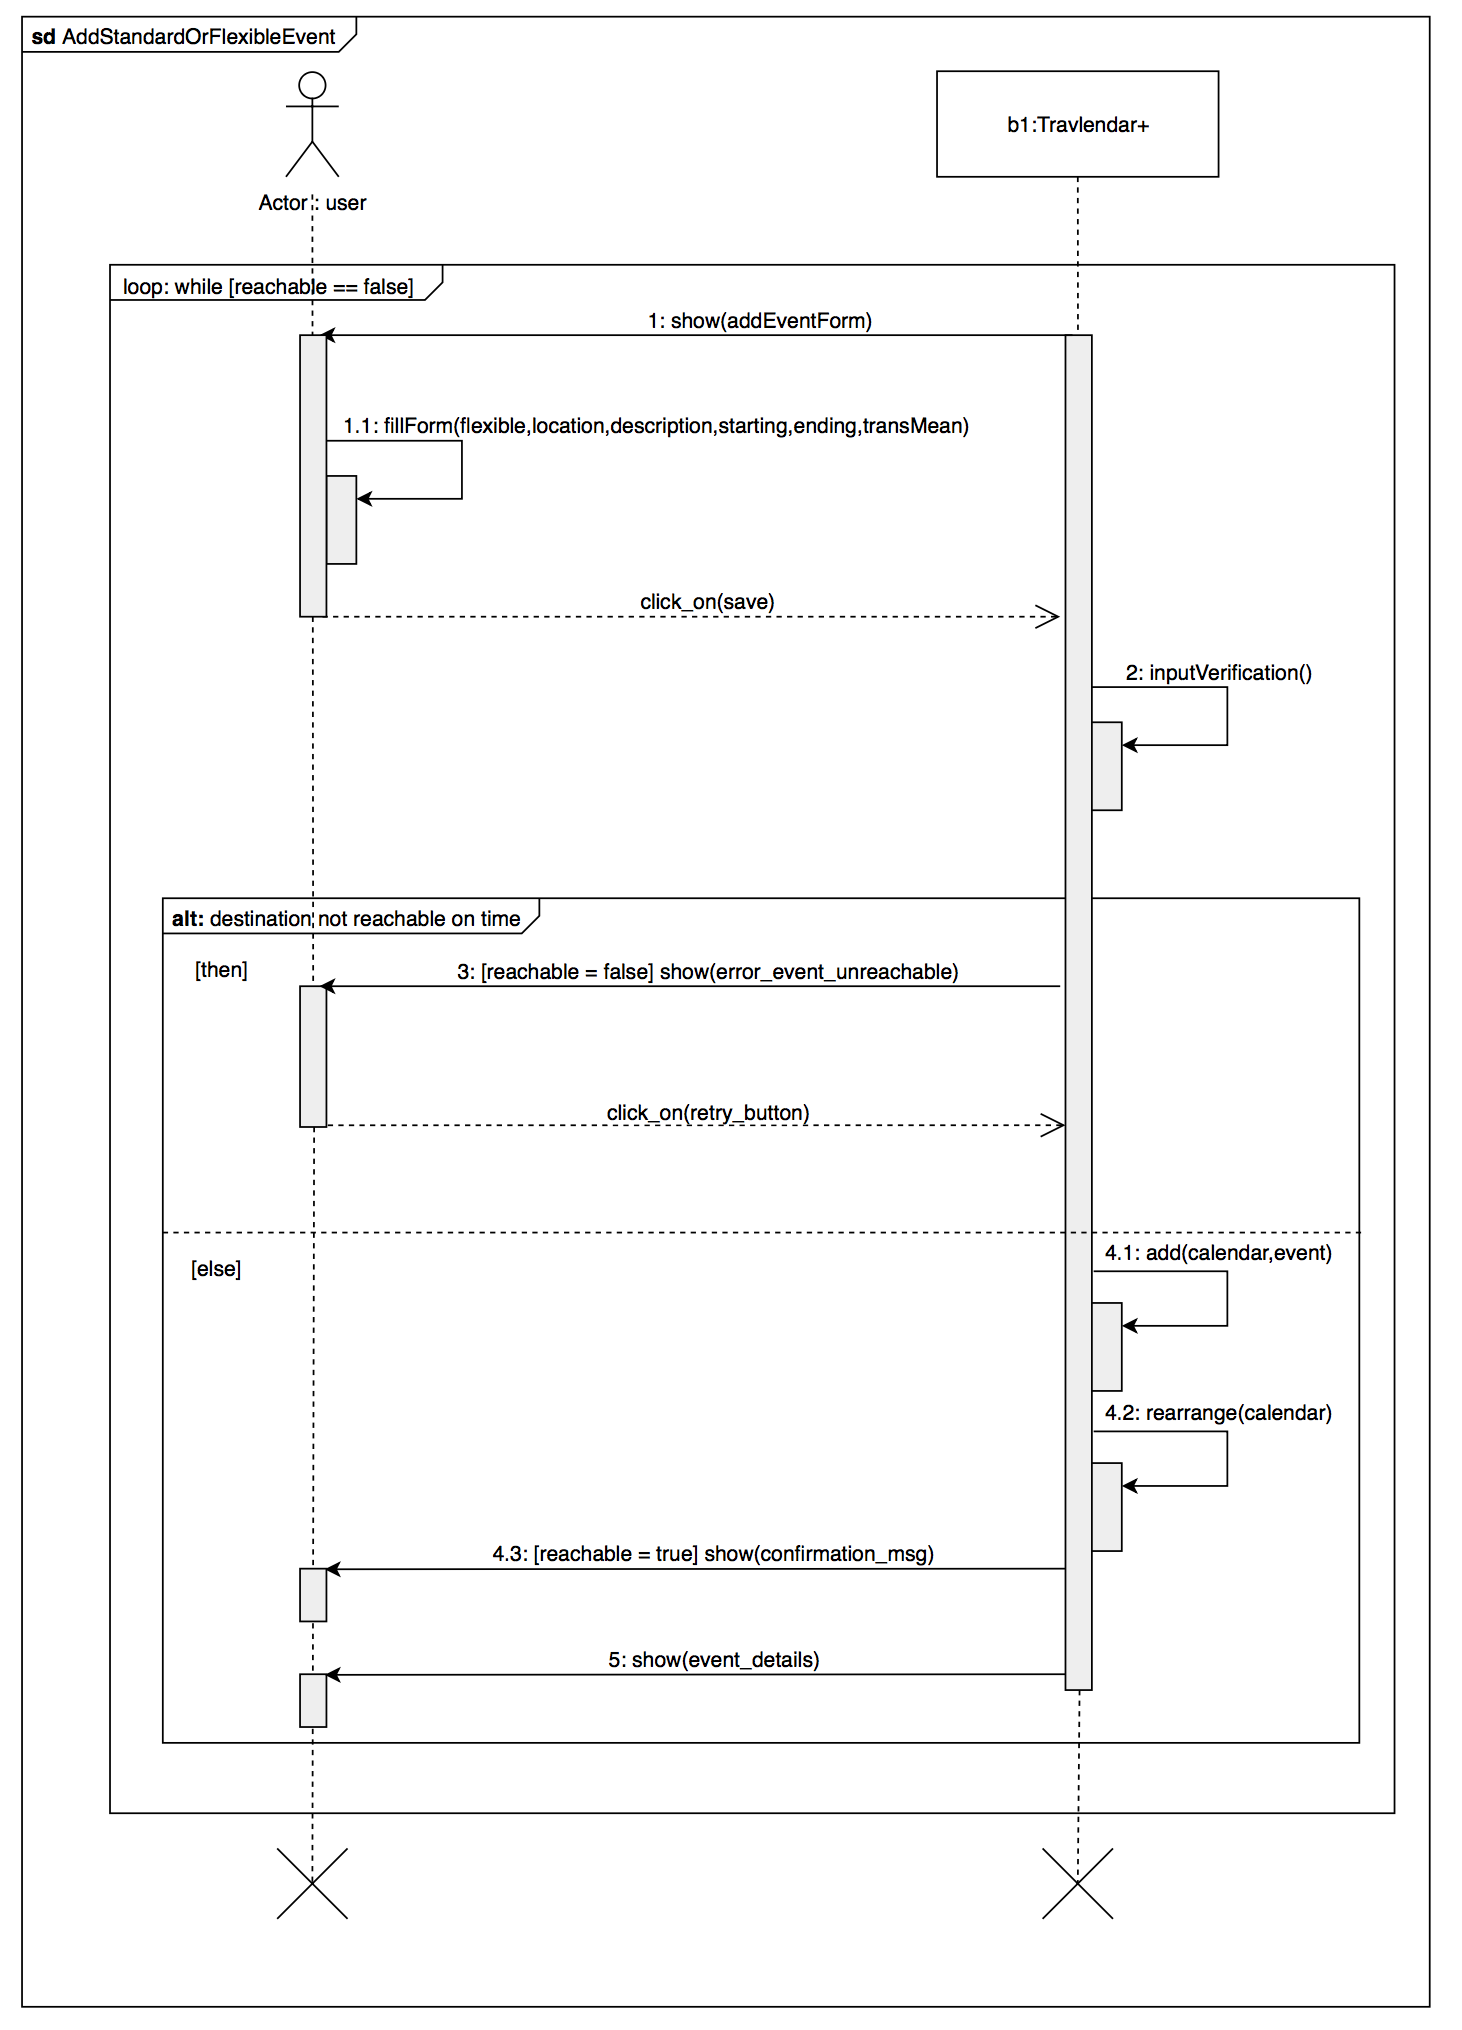
\includegraphics[scale=0.52]{images/SD/AddStandardFlexibleEvent}
\par\end{center}

\subsubsection{CreateCalendar}
\begin{center}
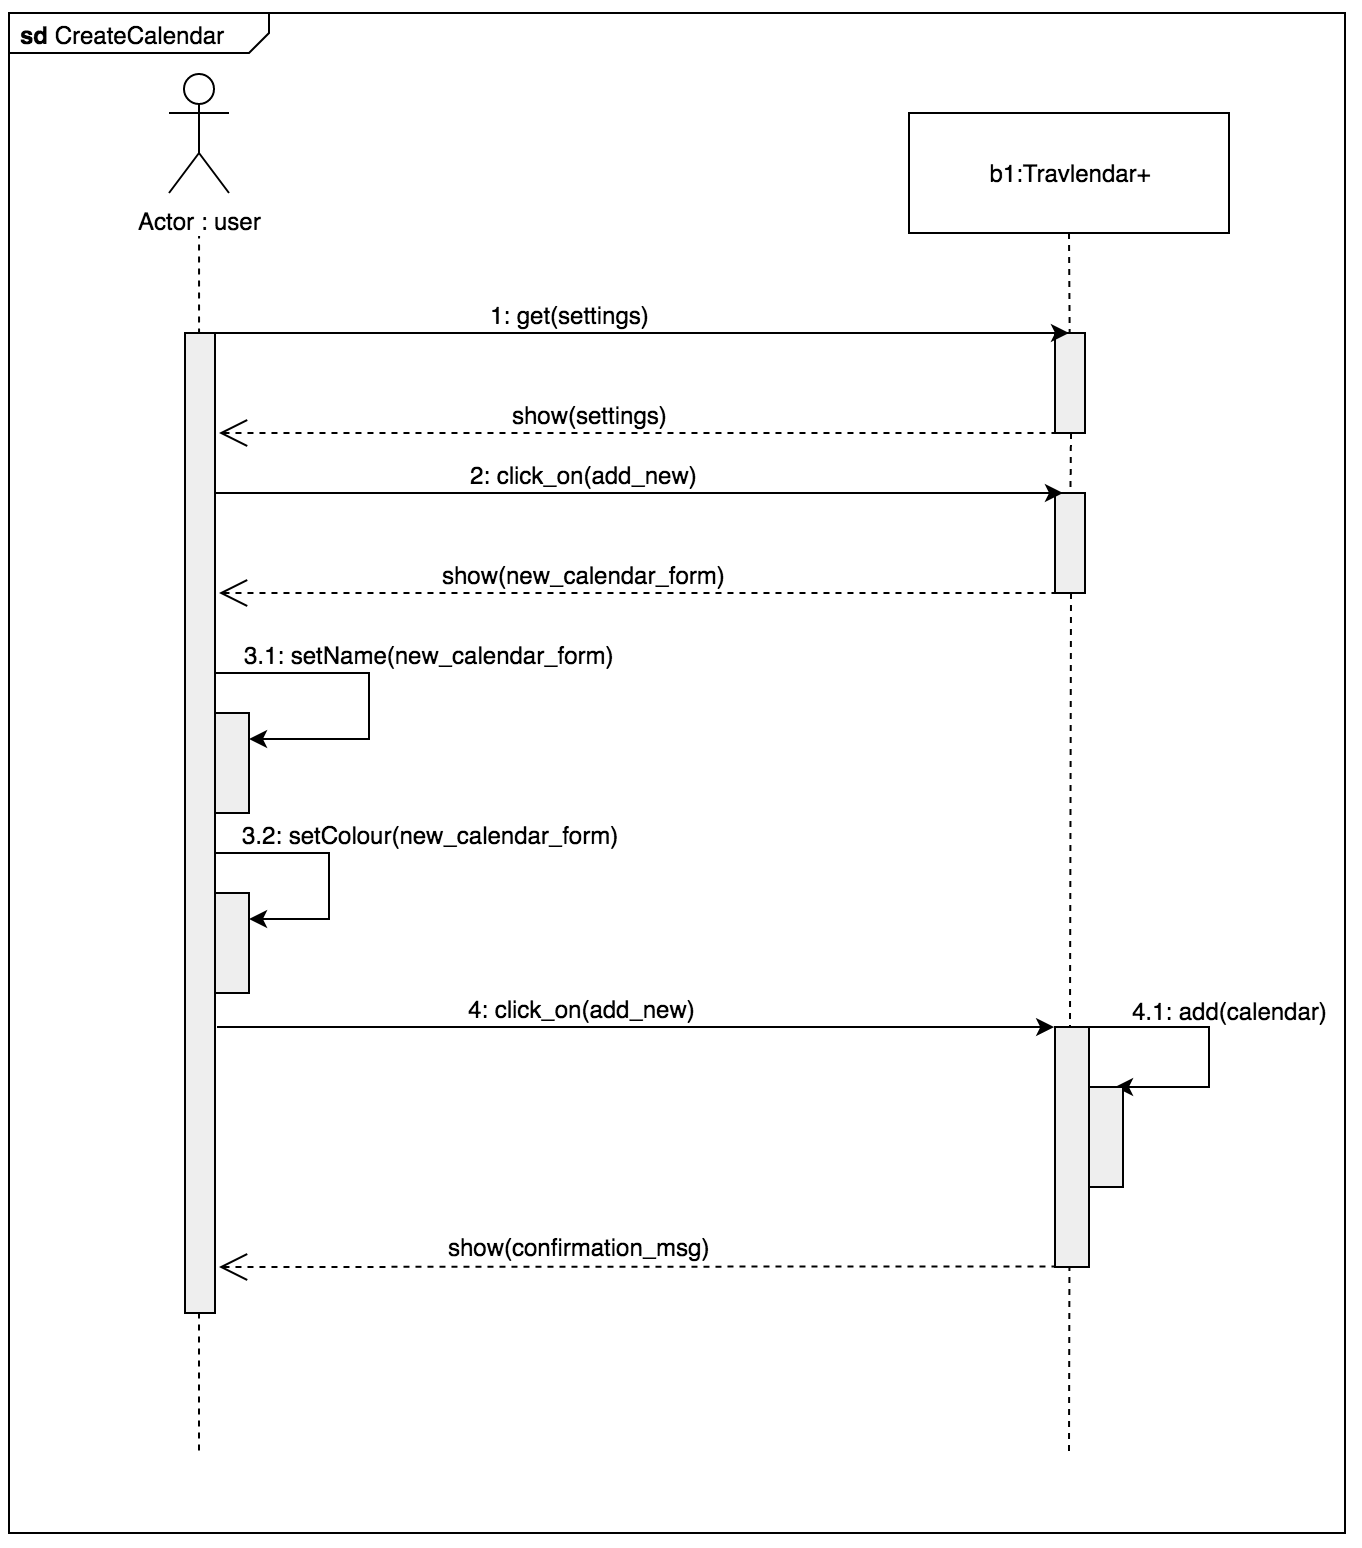
\includegraphics[scale=0.55]{images/SD/CreatCalendar}
\par\end{center}

\subsubsection{Edit Preferences}
\begin{center}
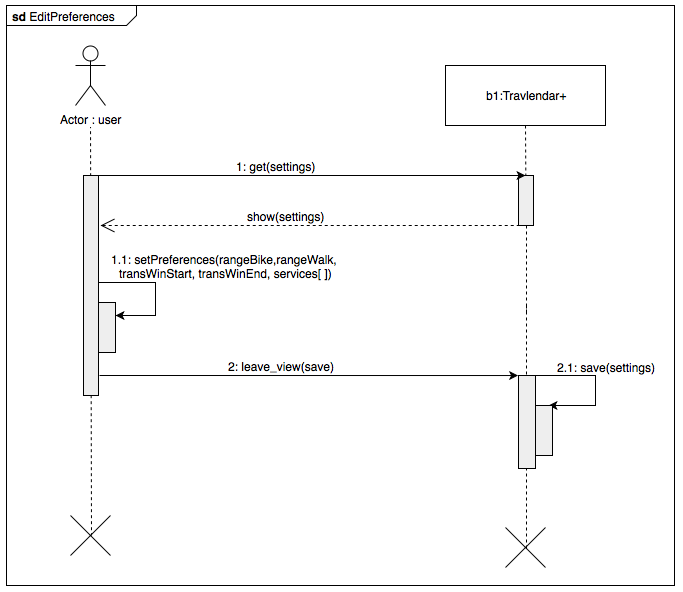
\includegraphics[scale=0.5]{images/SD/EditPreferences}
\par\end{center}

\subsubsection{BuyTickets}
\begin{center}
\hspace*{-3.5cm}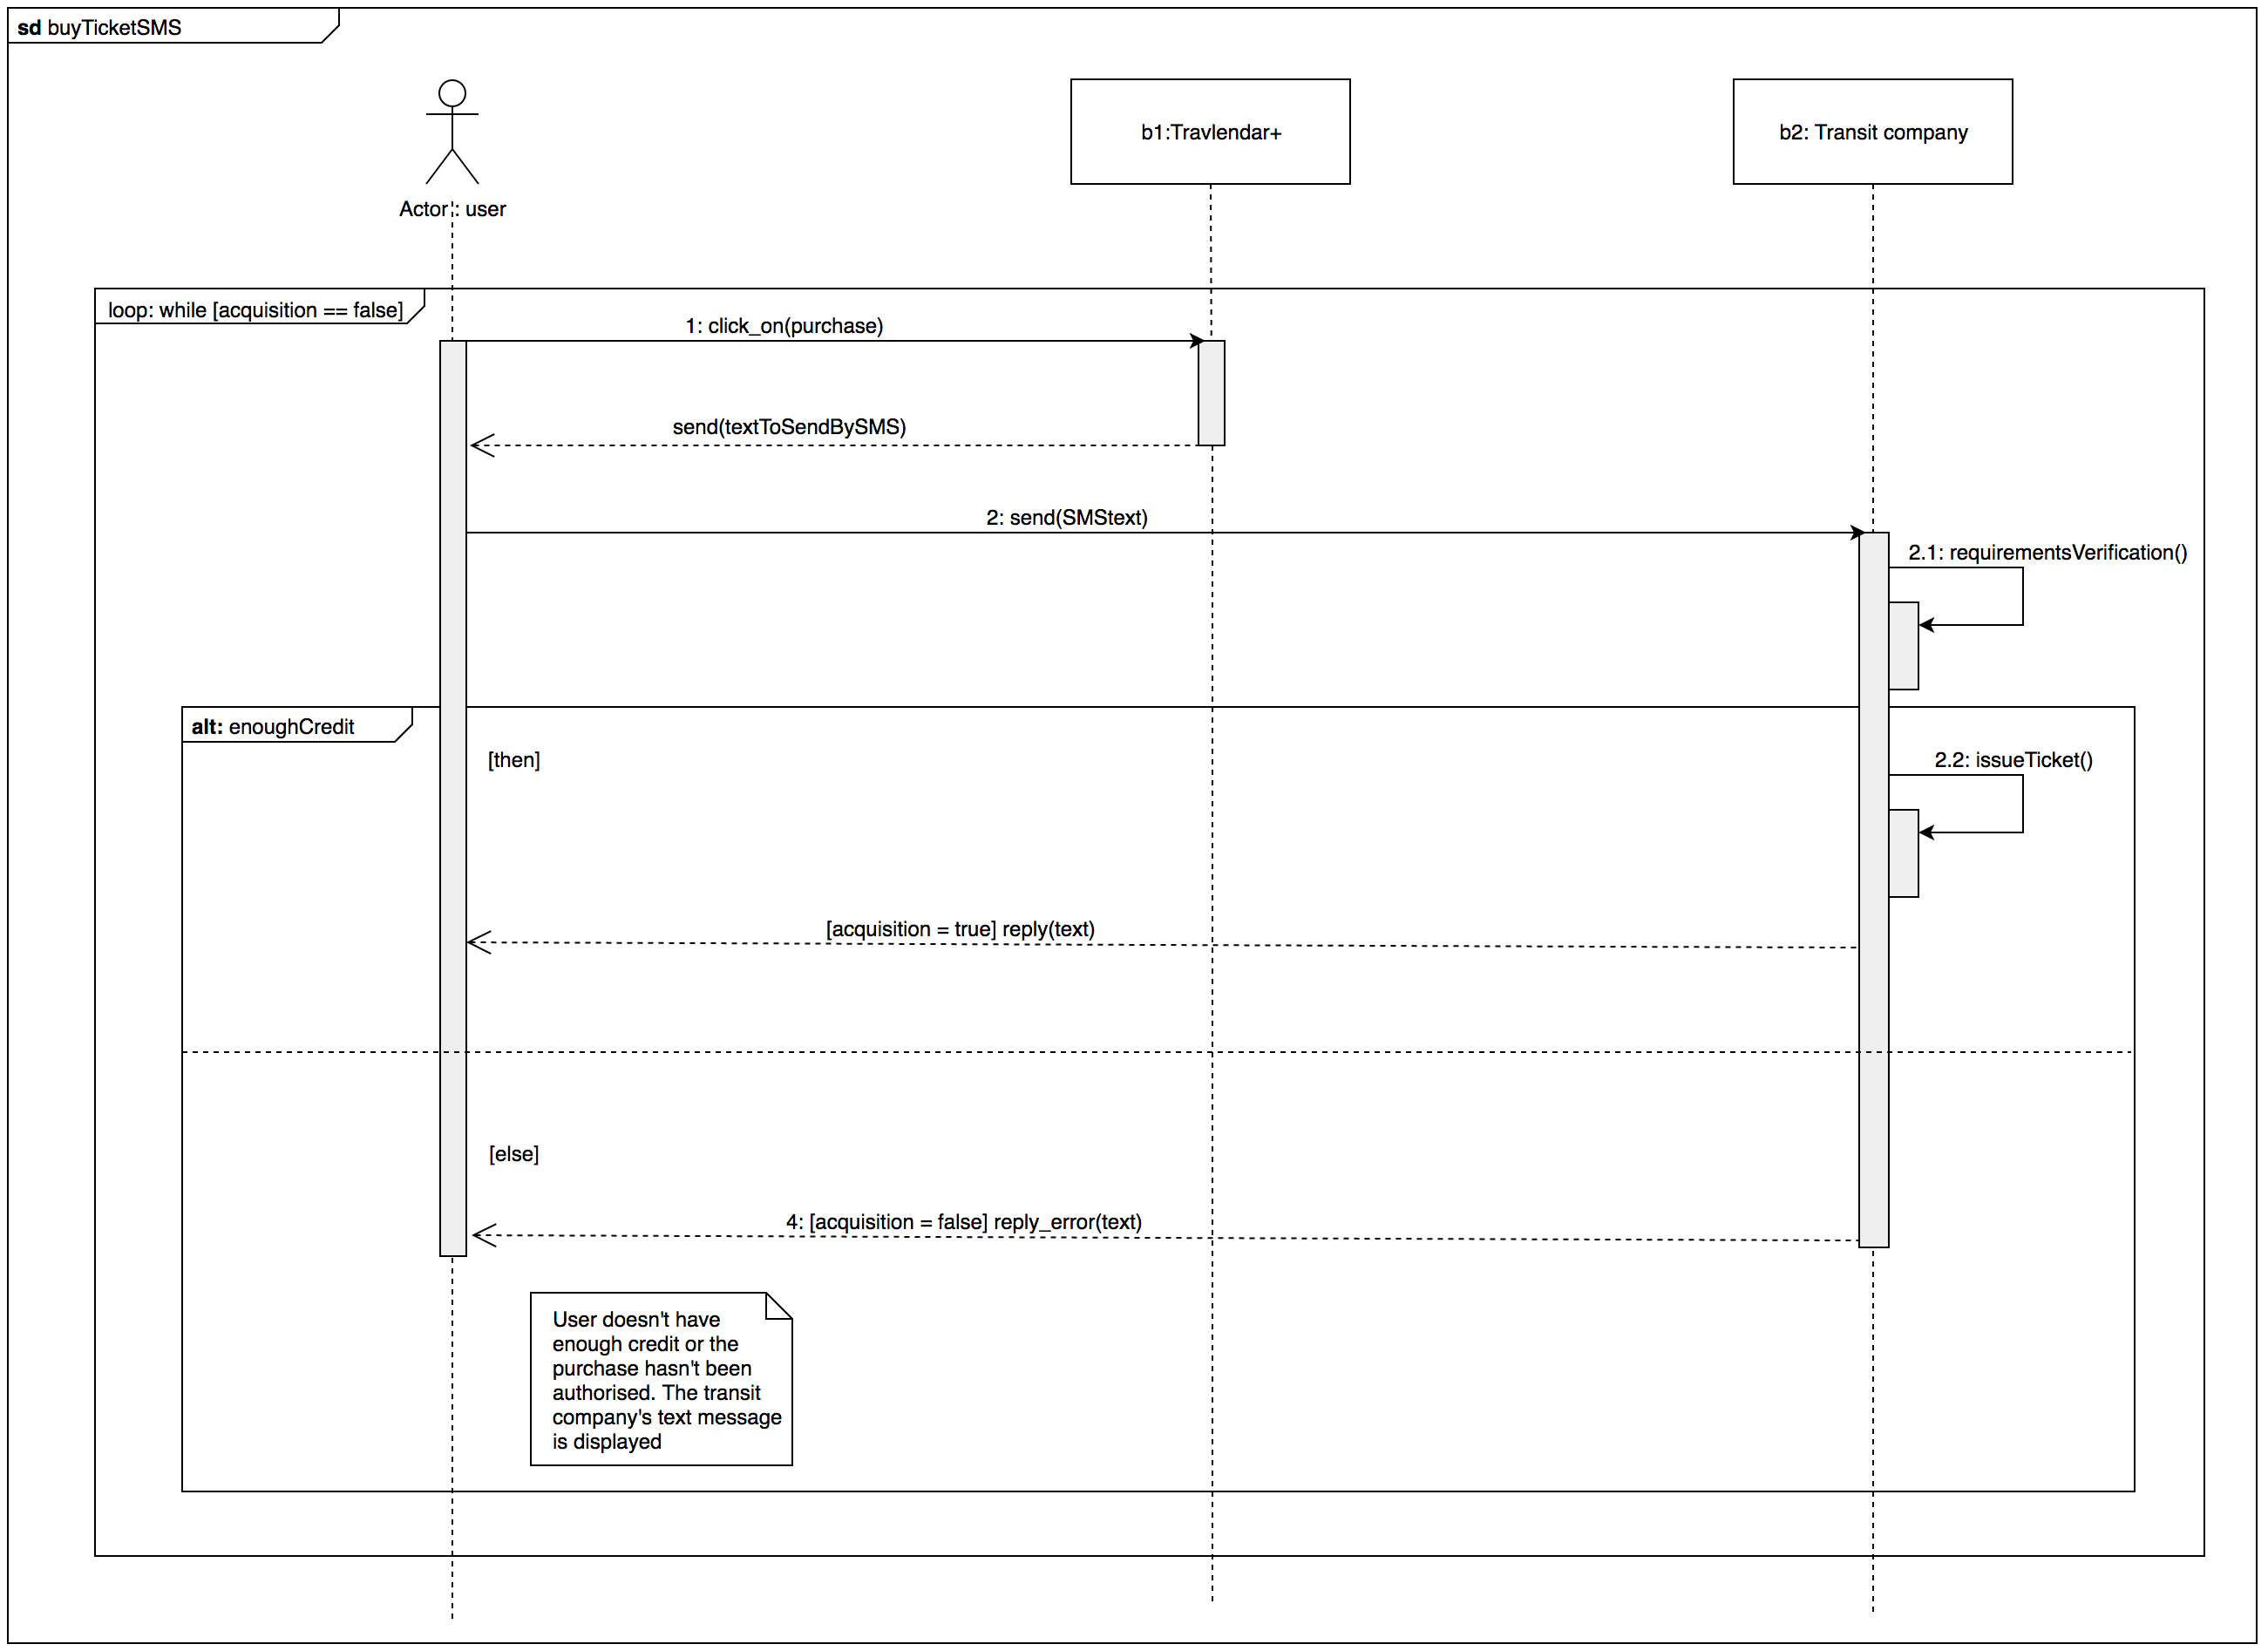
\includegraphics[scale=0.5]{images/SD/buyTicket}
\par\end{center}

\subsection{Use Case Diagram}
\begin{center}
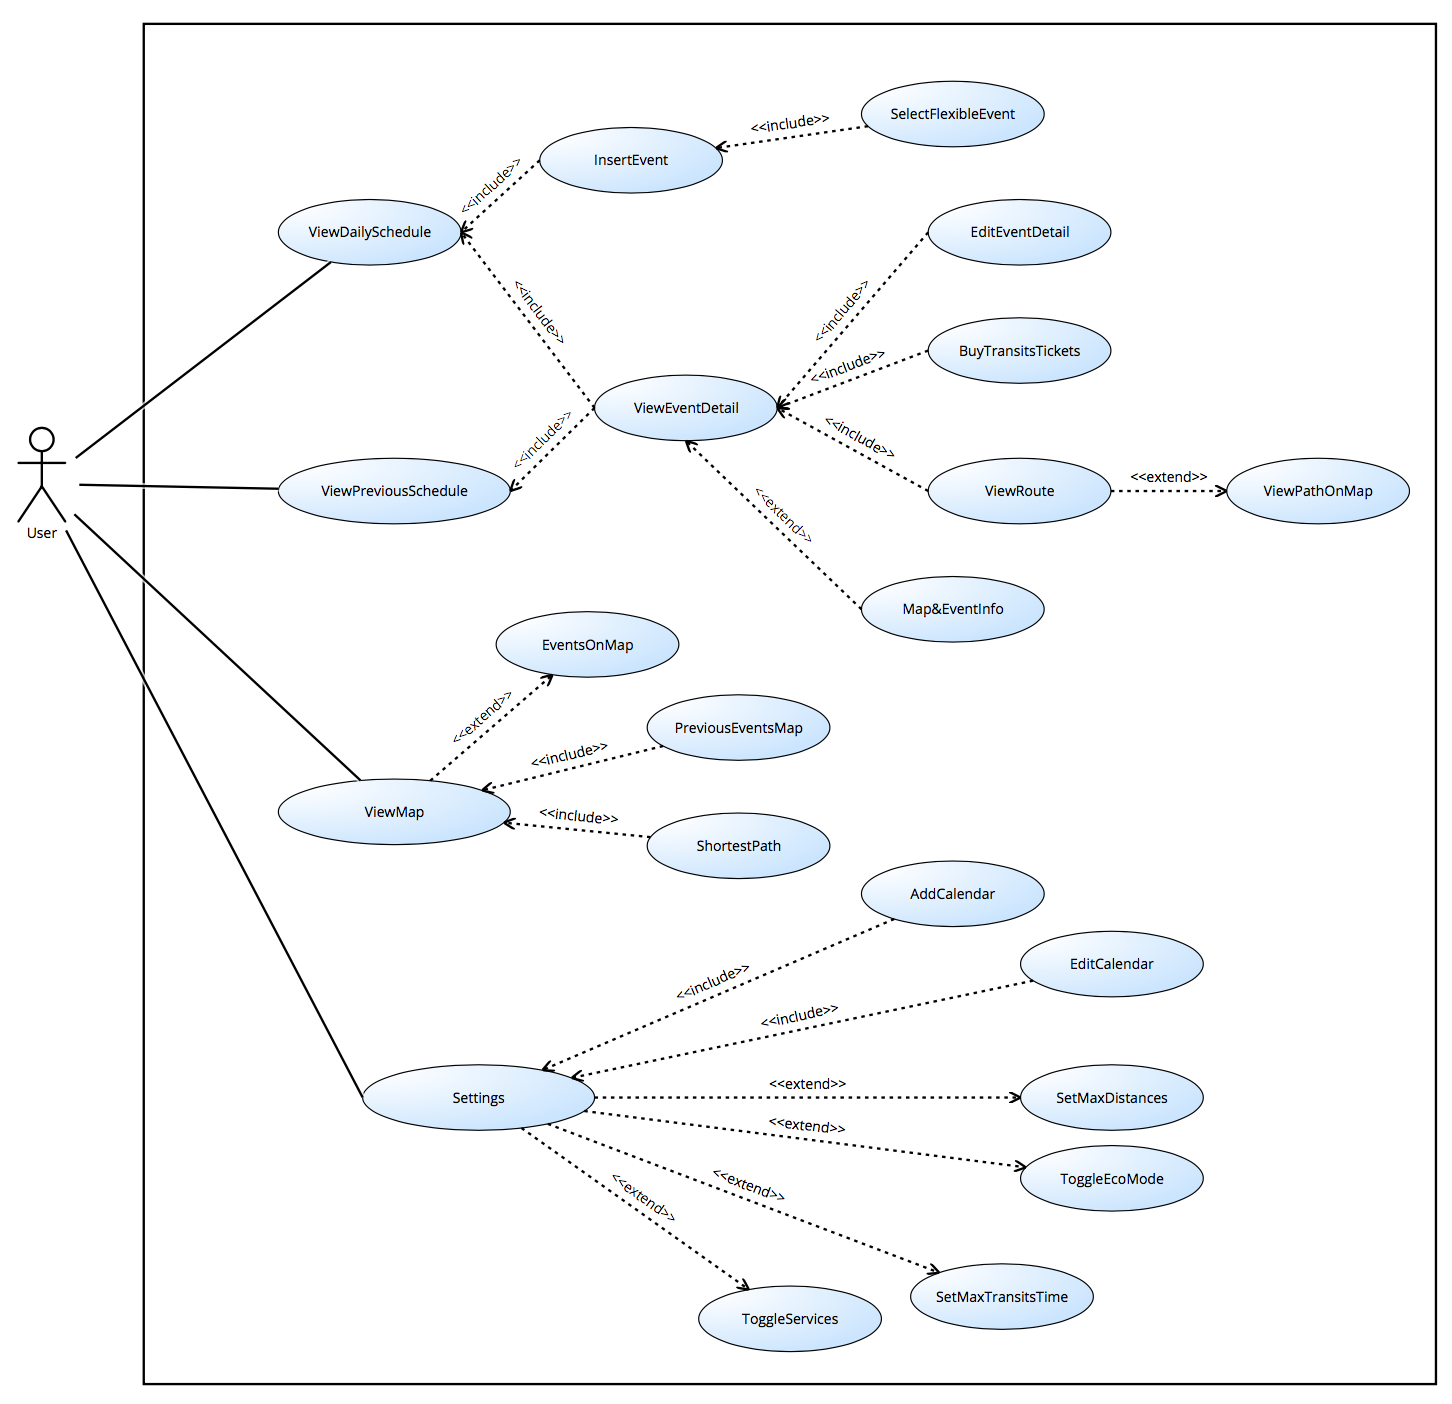
\includegraphics[scale=0.55]{images/UC}
\par\end{center}

\pagebreak{}

\subsection{Performance Requirements}

The system must be able to fulfill a big number of requests in the
shortest time possible. Approximately a request should not last more
than a second.

The server database should be fast enough to store and search data
in order of milliseconds even if million of records are stored.

The server should be located near the maximum concentration of final
users, in this case in Lombardy so that network latency will be minimized.

The application should not present any kind of lag in any situation
and should never crash.

\subsection{Design Constraints}

\subsubsection{Standards compliance}

The app must comply to the standard ``iOS Human Interface Guidelines''
and ``App Store Review Guidelines'' by Apple regarding the iOS App
and ``Google Play Guidelines'' for Android.

Regarding the interconnections between the app and the server the
system will use some APIs which will be REST-Compliant and they should
output data using XML or JSON.

\subsubsection{Hardware limitations}
\begin{itemize}
\item Mobile App 
\begin{itemize}
\item iOS, Android or Windows Phone Smartphone 
\end{itemize}
\item Connectivity
\begin{itemize}
\item 2G, 3G or LTE
\item GPS
\end{itemize}
\end{itemize}

\subsubsection{Any other constraint}

The system will ask the user permissions to get her/his current position.

The user won't require login because it will use the iCloud unique
identifier in order to synchronize events and calendars to the server.

\subsection{Software System Attributes}

\subsubsection{Reliability}

The system must guarantee a 24 hours per day and 7 days per week service.

The server should never be offline.

Very small deviations will be accepted only if the system will go
in maintenance mode.

\subsubsection{Availability}

The app will be available at worldwide level but can be used only
in Lombardy.

\subsubsection{Security}

The app will use the Cloud-Service unique identifier (iCloud, Google)
to identify the user also when he/she uninstalls the app and reinstalls
it.

This identifier is kept secret and it won't be stored on the server
for promotional or ambiguous purposes. Its intent is to identify the
user while using the system.

The app will communicate with the server via SSL certificates enabling
HTTPS secure requests.

\subsubsection{Maintainability}

The whole system will be developed using a modular architecture that
represents an important aspect to make it more maintainable and stable.

\subsubsection{Portability}

Portability will be highly guaranteed by distribution in OS such as
Android and iOS that represents 98\% of the smartphone market.

\pagebreak{}

\section{Formal analysis using Alloy}

\subsection{Signatures}

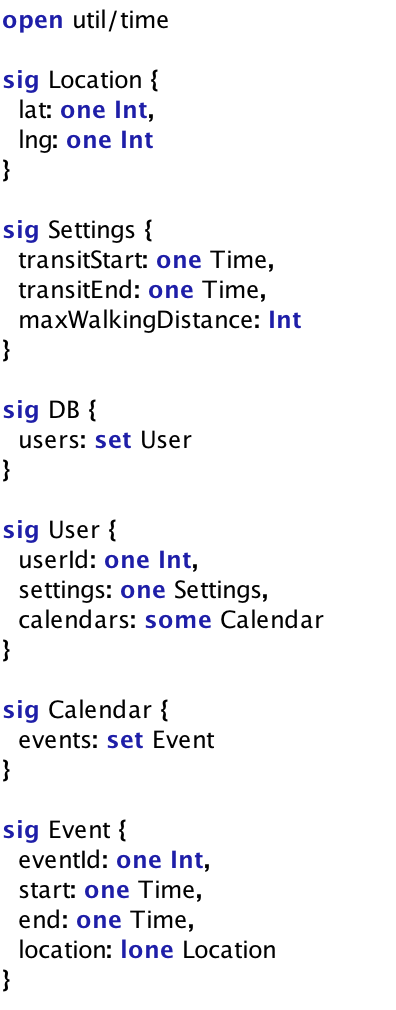
\includegraphics[scale=0.9]{images/alloy_sigs}

\pagebreak{}

\subsection{Facts}

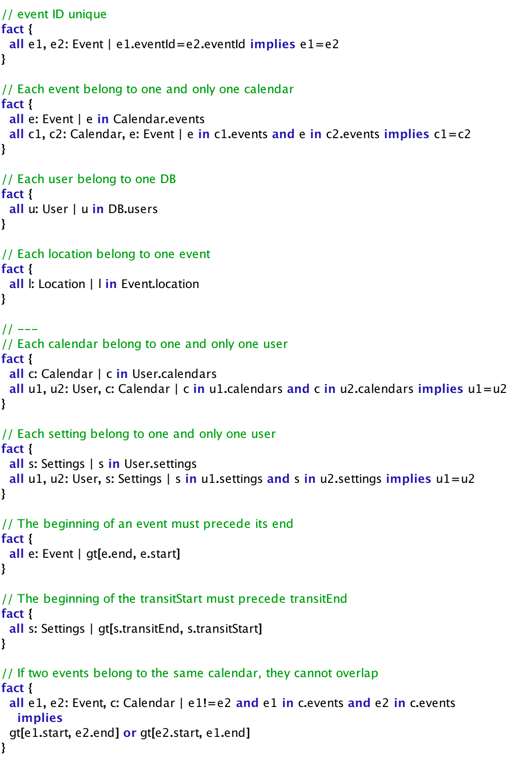
\includegraphics[scale=0.8]{images/alloy_facts}

\pagebreak{}

\subsection{Dynamic Model}

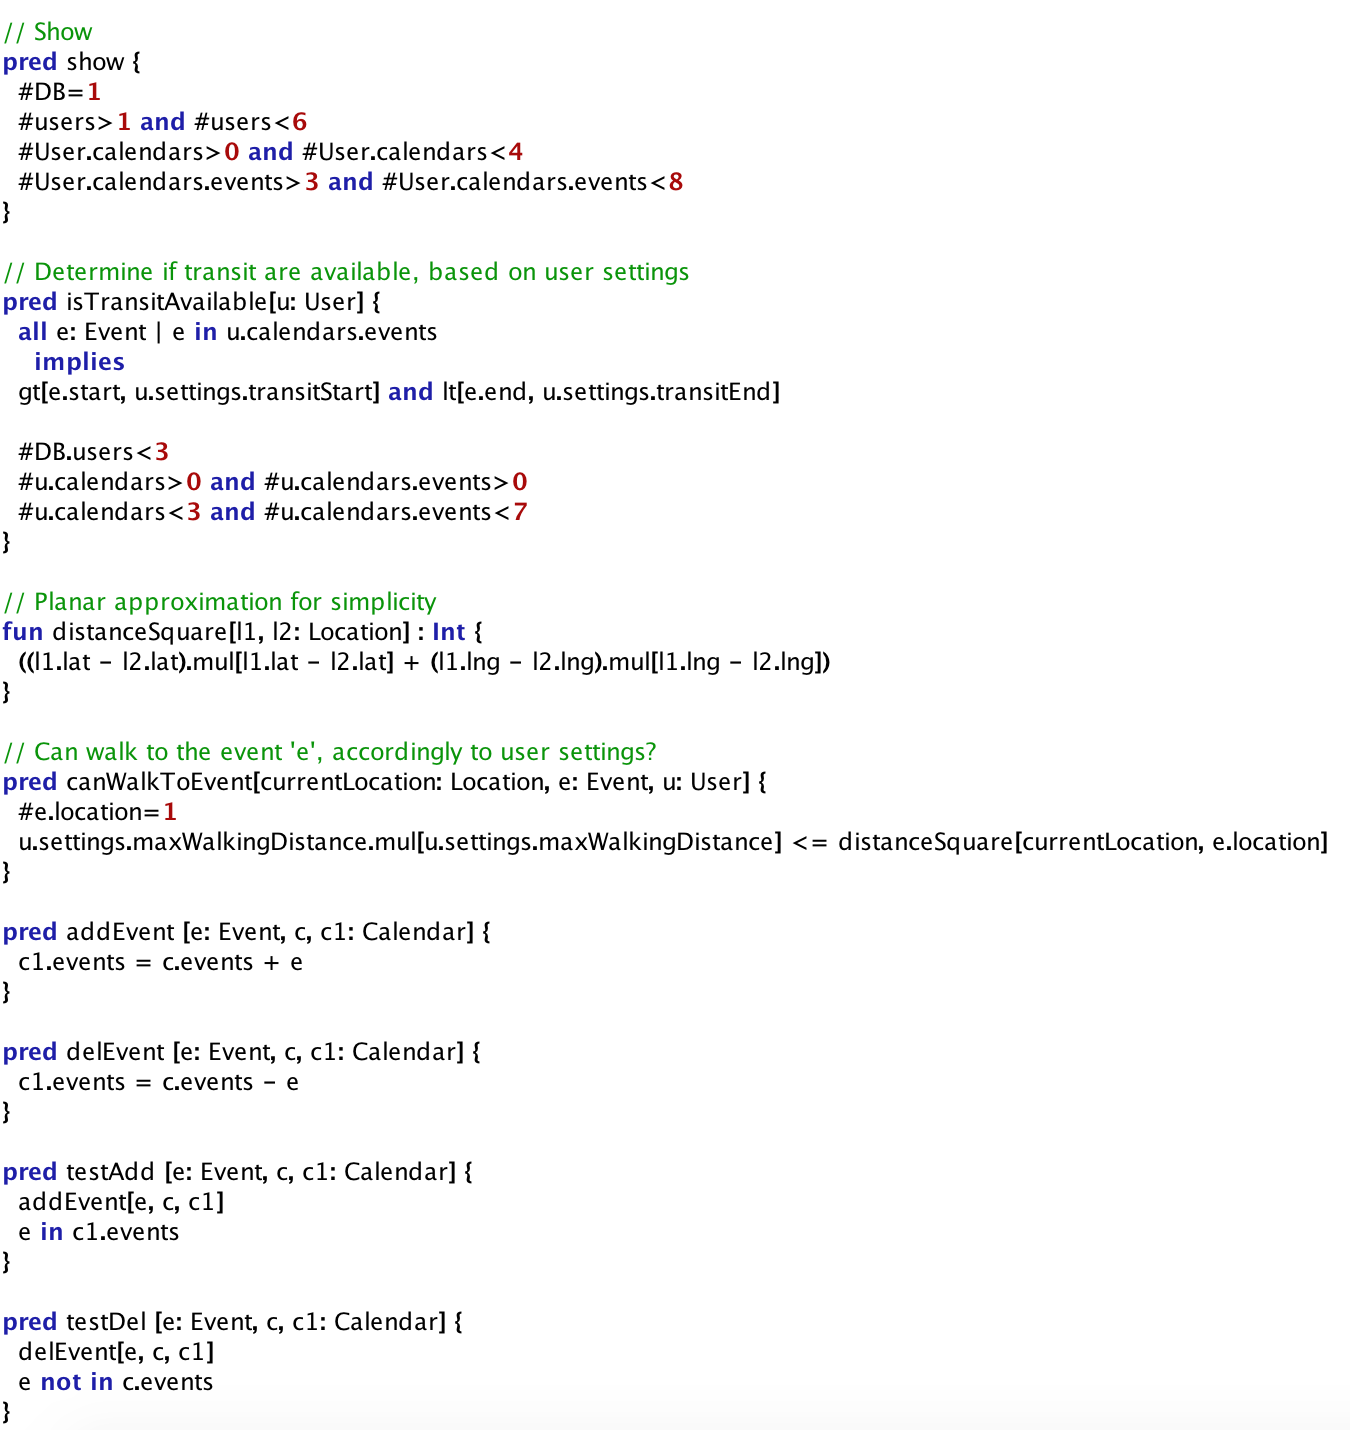
\includegraphics[scale=0.8]{images/alloy_preds}

\pagebreak{}

\subsection{Results}

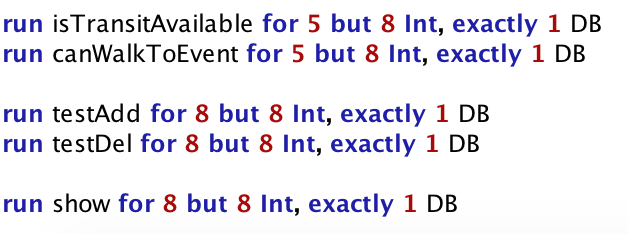
\includegraphics[scale=0.8]{images/alloy_results}

\subsubsection{Proof of Consistency}

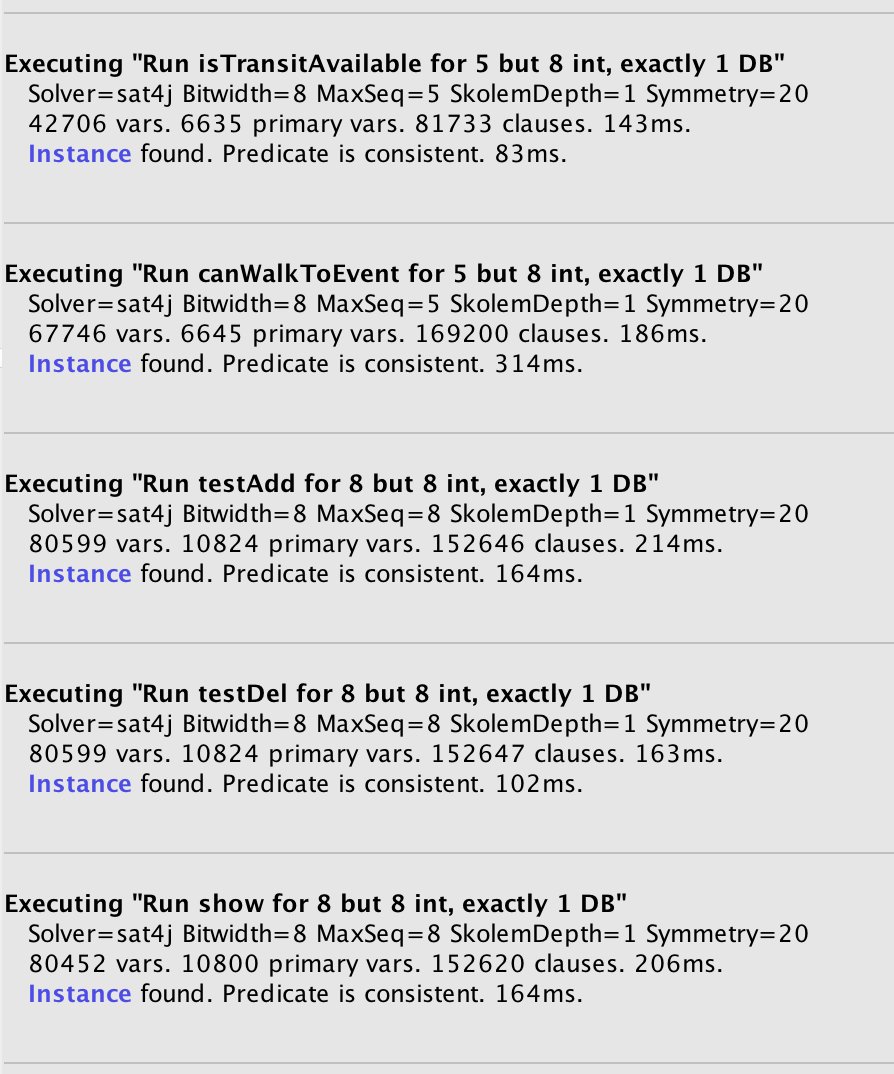
\includegraphics[scale=0.7]{images/alloy_proofs}

\subsubsection{Generated world}

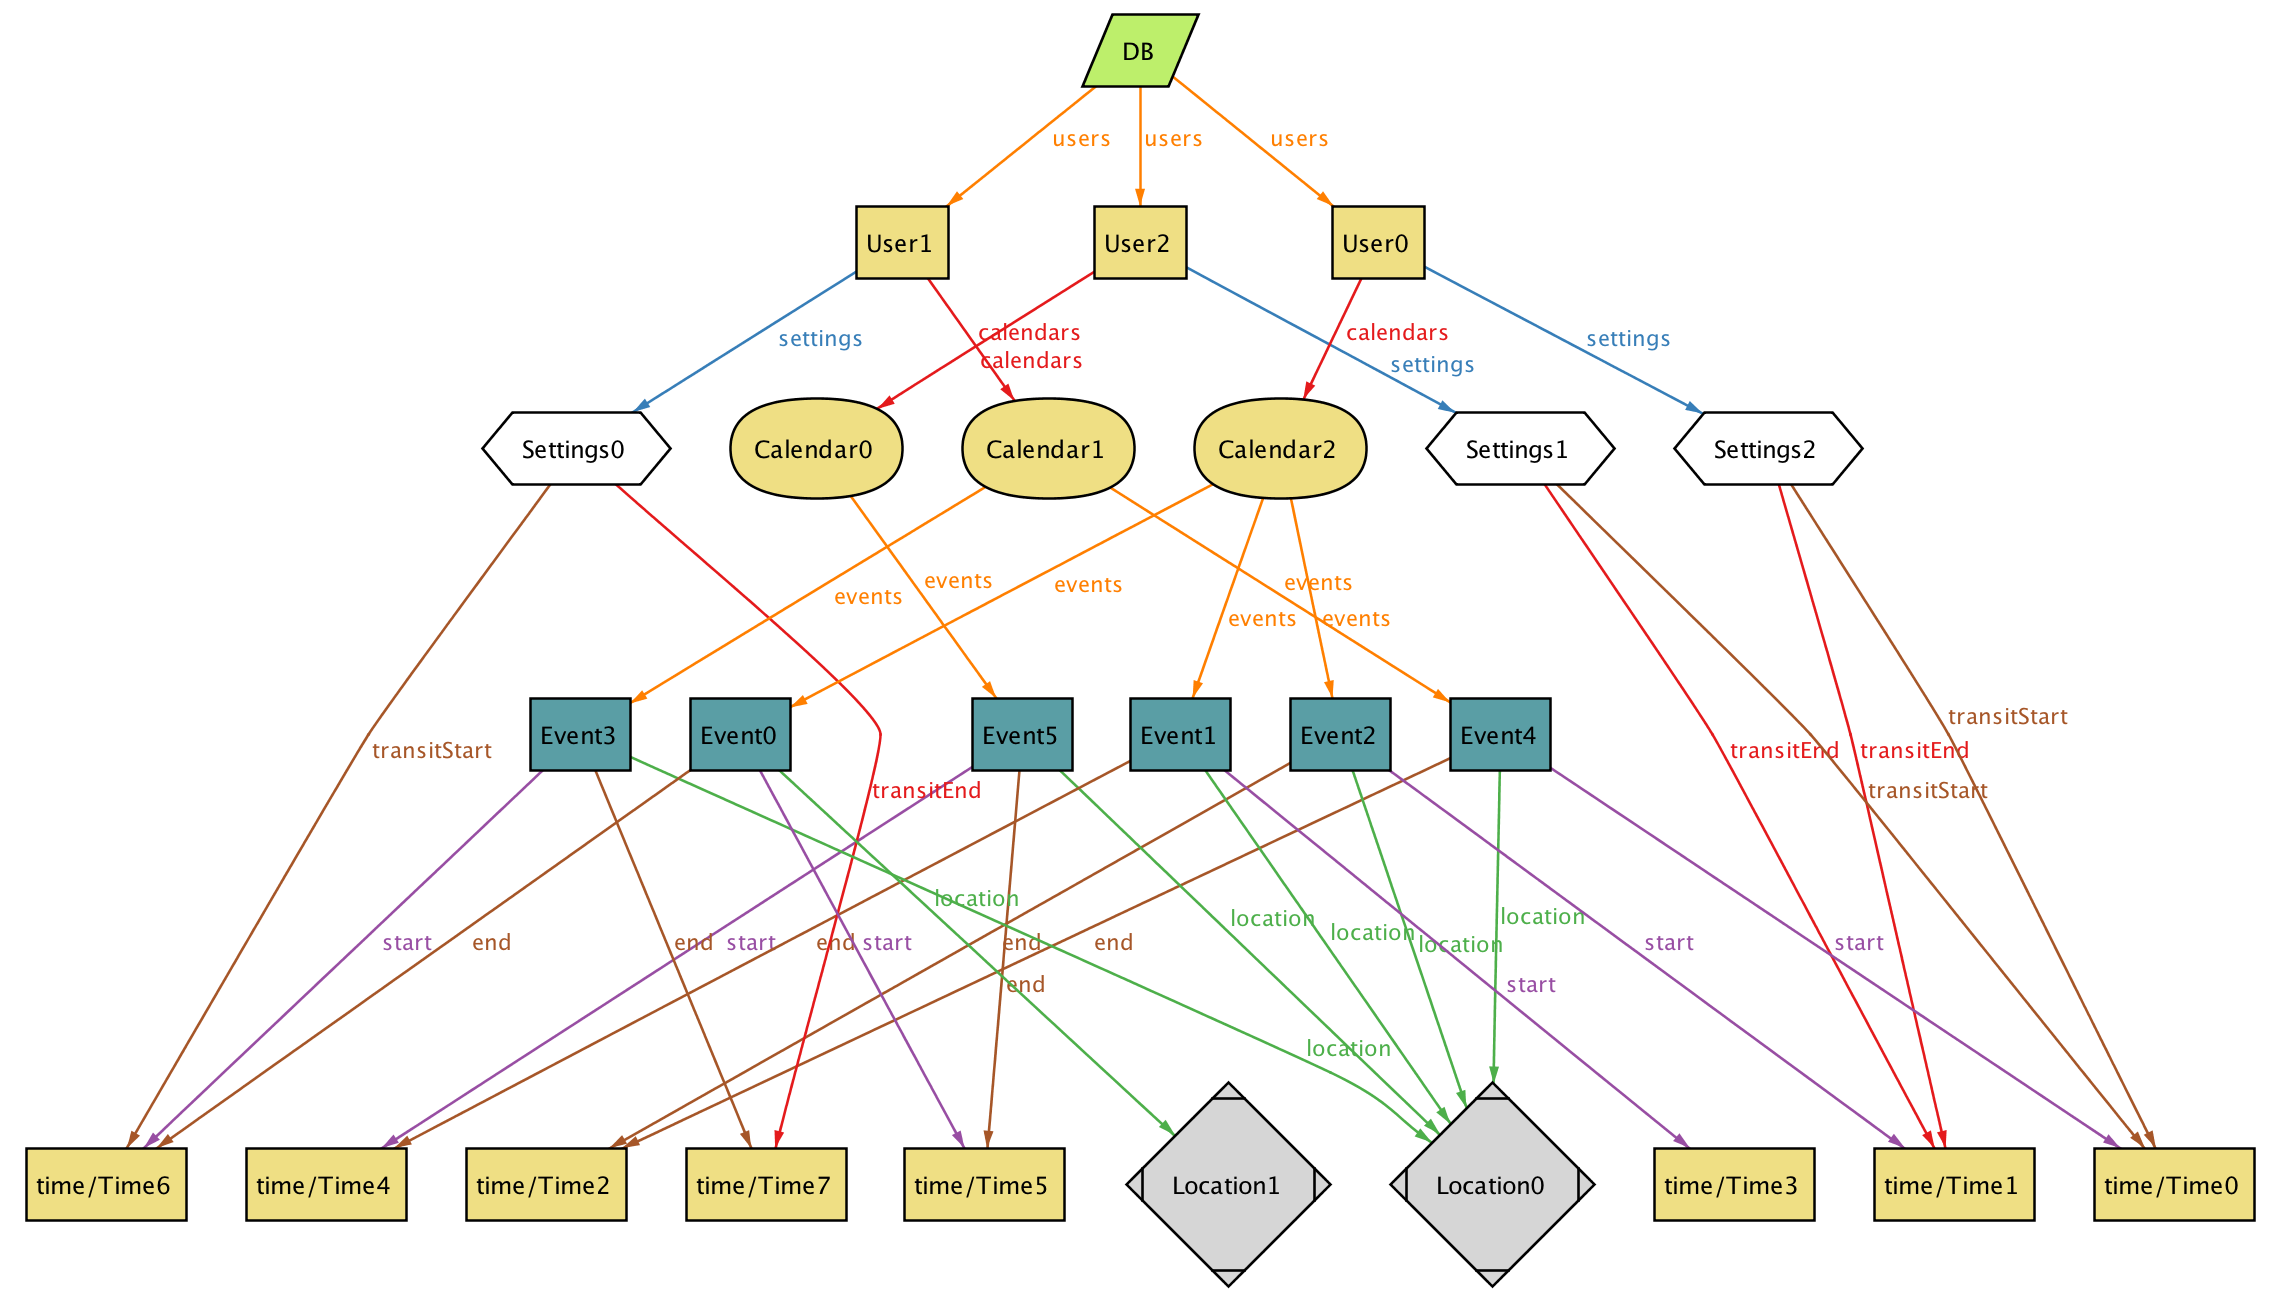
\includegraphics[angle=270,scale=0.5]{images/alloy_world}

\pagebreak{}

\section{Effort spent}
\begin{itemize}
\item Filippo Calzavara: 30.00h
\item Giovanni Filaferro: 30.00h
\item Benedetto Maria Nespoli: 30.00h
\end{itemize}

\section{References}
\begin{itemize}
\item iOS Human Interface Guidelines (https://developer.apple.com/ios/human-interface-guidelines/)
\item App Store Review Guidelines (https://developer.apple.com/app-store/review/guidelines/)
\item Google Play Guidelines (https://play.google.com/about/developer-content-policy/\#!?modal\_active=none)
\end{itemize}

\end{document}
